%%%%%%%%%%%%%%
%% Run LaTeX on this file several times to get Table of Contents,
%% cross-references, and citations.

%% If you have font problems, you may edit the w-bookps.sty file
%% to customize the font names to match those on your system.

%% w-bksamp.tex. Current Version: Feb 16, 2012
%%%%%%%%%%%%%%%%%%%%%%%%%%%%%%%%%%%%%%%%%%%%%%%%%%%%%%%%%%%%%%%%
%
%  Sample file for
%  Wiley Book Style, Design No.: SD 001B, 7x10
%  Wiley Book Style, Design No.: SD 004B, 6x9
%
%
%  Prepared by Amy Hendrickson, TeXnology Inc.
%  http://www.texnology.com
%%%%%%%%%%%%%%%%%%%%%%%%%%%%%%%%%%%%%%%%%%%%%%%%%%%%%%%%%%%%%%%%

%%%%%%%%%%%%%
% 7x10
%\documentclass{wileySev}

% 6x9

\documentclass{wileysix}
\UseRawInputEncoding
\usepackage{graphicx}
\usepackage{listings}
\usepackage{multirow}
\usepackage{float}

\usepackage{color}
 
\definecolor{codegreen}{rgb}{0,0.6,0}
\definecolor{codegray}{rgb}{0.5,0.5,0.5}
\definecolor{codepurple}{rgb}{0.58,0,0.82}
\definecolor{backcolour}{rgb}{0.95,0.95,0.92}
 
\lstdefinestyle{mystyle}{
    backgroundcolor=\color{backcolour},   
    commentstyle=\color{codegreen},
    keywordstyle=\color{magenta},
    numberstyle=\tiny\color{codegray},
    stringstyle=\color{codepurple},
    basicstyle=\footnotesize,
    breakatwhitespace=false,         
    breaklines=true,                 
    captionpos=b,                    
    keepspaces=true,                 
    numbers=left,                    
    numbersep=5pt,                  
    showspaces=false,                
    showstringspaces=false,
    showtabs=false,                  
    tabsize=2,
    language=sh
}
 
\lstset{style=mystyle}

%%%%%%%
%% for times math: However, this package disables bold math (!)
%% \mathbf{x} will still work, but you will not have bold math
%% in section heads or chapter titles. If you don't use math
%% in those environments, mathptmx might be a good choice.

% \usepackage{mathptmx}

% For PostScript text
\usepackage{w-bookps}

%%%%%%%%%%%%%%%%%%%%%%%%%%%%%%%%%%%%%%%%%%%%%%%%%%%%%%%%%%%%%%%%
%% Other packages you might want to use:

% for chapter bibliography made with BibTeX
% \usepackage{chapterbib}

% for multiple indices
% \usepackage{multind}

% for answers to problems
% \usepackage{answers}

%%%%%%%%%%%%%%%%%%%%%%%%%%%%%%
%% Change options here if you want:
%%
%% How many levels of section head would you like numbered?
%% 0= no section numbers, 1= section, 2= subsection, 3= subsubsection
%%==>>
\setcounter{secnumdepth}{3}

%% How many levels of section head would you like to appear in the
%% Table of Contents?
%% 0= chapter titles, 1= section titles, 2= subsection titles, 
%% 3= subsubsection titles.
%%==>>
\setcounter{tocdepth}{2}

%% Cropmarks? good for final page makeup
%% \docropmarks

%%%%%%%%%%%%%%%%%%%%%%%%%%%%%%
%
% DRAFT
%
% Uncomment to get double spacing between lines, current date and time
% printed at bottom of page.
% \draft
% (If you want to keep tables from becoming double spaced also uncomment
% this):
% \renewcommand{\arraystretch}{0.6}
%%%%%%%%%%%%%%%%%%%%%%%%%%%%%%

%%%%%%% Demo of section head containing sample macro:
%% To get a macro to expand correctly in a section head, with upper and
%% lower case math, put the definition and set the box 
%% before \begin{document}, so that when it appears in the 
%% table of contents it will also work:

\newcommand{\VT}[1]{\ensuremath{{V_{T#1}}}}

%% use a box to expand the macro before we put it into the section head:

\newbox\sectsavebox
\setbox\sectsavebox=\hbox{\boldmath\VT{xyz}}

%%%%%%%%%%%%%%%%% End Demo


\begin{document}
\booktitle{CodeIgniter : }
\subtitle{Implementasi Metode Entropy Pada Pemrograman PHP (Belajar Dengan Praktek)}

\authors{ M. Yusril Helmi Setyawan\\Cokro Edi Prawiro\\
\affil{Politeknik Pos Indonesia}
%Floyd J. Fowler, Jr.\\
%\affil{University of New Mexico}
}

\offprintinfo{Implementasi Metode Entropy Pada PHP, First Edition}{ M. Yusril Helmi Setyawan dan Cokro Edi Prawiro}

%% Can use \\ if title, and edition are too wide, ie,
%% \offprintinfo{Survey Methodology,\\ Second Edition}{Robert M. Groves}

%%%%%%%%%%%%%%%%%%%%%%%%%%%%%%
%% 
\halftitlepage

\titlepage

\begin{copyrightpage}{2020}
%Survey Methodology / Robert M. Groves . . . [et al.].
%\       p. cm.---(Wiley series in survey methodology)
%\    ``Wiley-Interscience."
%\    Includes bibliographical references and index.
%\    ISBN 0-471-48348-6 (pbk.)
%\    1. Surveys---Methodology.  2. Social 
%\  sciences---Research---Statistical methods.  I. Groves, Robert M.  II. %
%Series.\\
%
%HA31.2.S873 2007
%001.4'33---dc22                                             2004044064
\end{copyrightpage}

\dedication{`Jika Kamu tidak dapat menahan lelahnya belajar, 
Maka kamu harus sanggup menahan perihnya Kebodohan.'
~Imam Syafi'i~}

\begin{contributors}
\name{M. Yusril Helmi Setyawan., Cokro Edi Prawiro} Diploma 4 Teknik Informatika., Politeknik Pos Indonesia, Bandung,
Indonesia



\end{contributors}

\contentsinbrief
\tableofcontents
\listoffigures
\listoftables
\lstlistoflistings


\begin{foreword}
Terimakasih penulis ucapkan kepada kaprodi D-IV Teknik Informatika, bagian kemahasiswaan, serta khususnya mahasiswa D-IV Teknik Informatika yang telah membantu proses penulisan dalam buku ini.
\end{foreword}

\begin{preface}
Alhamdulillah, segala puji dan syukur penulis panjatkan kehadirat Allah SWT karena buku ini telah selesai disusun. Buku ini di susun dengan tujuan untuk memberitahu cara penerapan metode entropy pada pemerograman php khususnya menggunakan faramwork codeigniter sebagai framework dari php itu sendiri.\par

Penusis menyadari bahwa jika dalam penyusunan buku ini masih mempunyai kekurangan, namun penulis menyakini bahwa sekecil apapun ilmu yang terdapat pada buku ini pasti bermanfaat bagi para pembaca\par


Akhir kata , maka kritik dan saran sangat berguna untuk penulis.

\prefaceauthor{Penulis}
\where{Bandung, Jawa Barat\\
Maret, 2020}
\end{preface}


\begin{acknowledgments}
Terima kasih atas masukan dan bimbingannya dari dosen pembimbing agar bisa membuat buku ini menjadi lebih baik dan lebih mudah di mengerti.\\

kemudian terimakasih saya ucapkan kepada keluarga terutama orang tua yang telah mendukung dalam pembuatan buku ini sehingga buku ini dapat di selesaikan.\\

terima kasih ini juga di tujukan kepada teman-teman mahasiswa yang telah memberikan masukan dan sarn dalam membuat buku ini, terimakasih juga saya ucapkan kepada team IRC yang telah membantu dalam pembuatan buku ini \\




\authorinitials{C. E. P. dan M. Y. H. S}
\end{acknowledgments}

\begin{acronyms}
\acro{CRUD}{Create Read Update Delete}
\acro{DBMS}{Database Management System}
\acro{OOP}{Object Oriented Programming}
\acro{DM}{Decision Matrix}
\end{acronyms}

\begin{glossary}
\term{Entropy}Merupakan Metode untuk menentukan bobot dari kriteria

\term{USER}Merupakan Pengguna dari sistem

\term{USER ADMIN}Menggunakan user dari pengguna sistem yang memiliki hakakses lebih daripada pengguna lain

\term{Source Code}Merupakan code-code yang di gunakan pada sistem baik itu bahasa pemerograman PHP maupun yang lainnya.
\end{glossary}

%\begin{symbols}
%\term{A}Amplitude

\term{\hbox{\&}}Propositional logic symbol 

\term{a}Filter Coefficient\cite{raharjo2015belajar}

\bigskip

\term{\mathcal{B}}Number of Beats
%\end{symbols}

\begin{introduction}

%% optional, but if you want to list author:

\introauthor{ M. Yusril Helmi Setyawan., Cokro Edi Prawiro}
{Informatics Research Center\\
Bandung, Jawa Barat, Indonesia}

Metode Entropy merupakan metode yang digunakan untuk menentukan bobot dari keriteria-keriteria yang terdiri dari beberapa alternatif kemudian untuk CodeIgniter merupakan framework untuk pemerograman PHP yang pada buku ini digunakan sebagai tools untuk menerapkan metode Entropy pada sistem yang di bahas pada buku ini.

\end{introduction}

%%%%%%%%%%%%%%%%%%Isi Buku_

\chapter{CodeIgniter}
%%\chapter{\textit{Python}}%%

pada bab in yang akan di bahas yaitu mengenai sejarah singkat dari \textit{Framework CodeIgniter}, kemudian keunggulan dari \textit{Framework CodeIgniter},
kemudian sarana untuk memperajari \textit{Framework CodeIgniter}, kemudian alat pendukung untuk menggunakan \textit{Framework CodeIgniter} lalu dilanjutkan dengan penjelasan singkat tentang MVC 
pada \textit{Framework CodeIgniter} setelah itu penjelasan tentang direktori pada paket yang telah di sediakan oleh \textit{Framework CodeIgniter}, terakhir merupakan editor teks yang dianjurkan
 untuk \textit{Framework CodeIgniter} serta contoh implementasi MVC sederhana.\pagebreak

\section{Sejarah \textit{CodeIgniter}}
Codeigniter merupakan \textit{faramework} web yang digunakan untuk bahasa pemerograman PHP yang dibuat oleh Rick Ellis pada tahun 2006 tepatnya pada tanggal 28 Febuari 2006,  penemu dan pendiri Ellis Lab (www.ellislab.com). Ellislab merupakan suatu tim kerja yang berdiri pada tahun 2002 dan bergerak di bidang pembuatan software dan tool untuk para pengembang web. Kemudian pada bulan Juli 2013 Ellis Lab mereka mengumumkan mencari pemilik baru untuk \textit{CodeIgniter} yang dikarenakan pada lingkup internal tidak memiliki fokus untuk mengembangkan \textit{CodeIgniter}, kemudian pada tahun 2014 tepatnya pada bulan oktober 2014 sampai sekarang, EllisLab telah menyerahkan hak kepemilikan \textit{CodeIgniter} ke \textit{British Columbia Institute of Technology} (BCIT) yang merupakan sekolah tinggi teknologi di kanada, untuk proses pengembangan lebih lanjut. Saat ini situs resmi \textit{CodeIgniter} telah berubah dari \textit{www.ellislab.com} ke \textit{www.codeigniter.com.} \cite{raharjo2015belajar}. \par

Setelah kurang lebih lima bulan setelah berpindah kepemilikan, BCIT akhirnya merilis \textit{CodeIgniter} versi 3.0, yang jika dibandingkan dengan versi sebelumnya tentunya \textit{CodeIgniter} 3 memiliki fitur yang lebih kaya seperti pengembangan \textit{database driver}, terdapat pustaka-pustaka baru dan juga PDO \textit{CodeIgniter} yang telah berfungsi secara penuh dengan subdriver \cite{subagia2018kolaborasi}.\par

Dibandingkan web \textit{faramework} yang lain \textit{CodeIgniter} memiliki desain yang lebih sederhana dan bersifat tidak kaku (fleksibel). \textit{CodeIgniter} masih mengizinkan atau memberikan kebebasan kepada para pengembang untuk menulis code-code tertentu di dalam aplikasi menggunakan cara konvesional atau tanpa menggunakan \textit{faramework} \cite{david2017codeigniter}.\par

Ditulis padadokumentasi \textit{CodeIgniter}, \textit{CodeIgniter} juga merupakan tollkit bagi orang atau perogramer yang ingin membangun aplikasi web menggunakan PHP. Tujuannya adalah membuat pengembangan proyek menjadi lebih cepat daripada membuat code dari awal. Pada \textit{CodeIgniter} juga memberikan kumpulan library untuk program yang sering di gunakan dan untuk mengakses library tersebut terbilang cukup mudah, dengan menggunakan framework codeigniter kita tinggal fokus pada pengembangan sistem atau projek serta meminimalisir jumlah kode yang akan dibuat.\pagebreak

\section{Beberapa Keuntungan \textit{CodeIgniter}}
CodeIgniter merupakan toolkit untuk orang-orang yang ingin membuat atau membangun aplikasi web menggunakan bahasa pemerograman PHP. Adapun beberapa keunggulan yang di tawarkan oleh CodeIgniter adalah sebagai \cite{raharjo2015belajar} , \cite{subagia2018kolaborasi} berikut:\par

\begin{enumerate}
\item \textit{CodeIgniter} merupakn framework yang bersipat gratis atau open-source
\item \textit{CodeIgniter} memiliki ukuran file yang relatif kecil dibandingkan Framework php lain. Setelah di download dan di ekstrak file codeigniter memiliki total ukuran kurang lebih 11 MB dengan ketentuan folder user guide (dokumentasi \textit{CodeIgniter}) kurang lebih sebesar 9 MB dan folder aplikasi dan sistem dengan ukurang kurang lebih 2 MB 
\item Aplikasi yang dibuat menggunakan codeigniter dapat berjalan dengan cepat
\item \textit{CodeIgniter} Menggunakan pola desain Model-View-Controller (MVC) yang memungkinkan pada satu file tidak akan berisi banyak code. Halini mengakibatkan kode menjadi mudah untuk di baca, dipahami dan dikembangkan atau dilakukan maintaining (pemeriharaan) di kemudian hari.
\item \textit{CodeIgniter} dapat diperluas sesuai dengan kebutuhan.
\item \textit{CodeIgniter} juga terdokuntasi dengan baik atau memiliki dokumentasi yang sangat baik. Informasi tentang class dan function yang terdapat pada codeigniter dapat diperoleh melalui dokumentasi yang disediakan pada paket distribusinya.
\item \textit{Pack a Punch}, \textit{CodeIgniter} hadir dengan \textit{library} yang akan membantu tugas-tugas di pengembangan web yang sudah umum dan sering di lakukan seperti mengakses basis data, mengirim email, validasi data dari form, mengelola session, memanipulasi gambar,  dan masih banyak lagi yang lainnya.
\item \textit{Extensible}kita dapat menambahkan \textit{library} atau \textit{helper} yang di ciptakan sendiri kemudian di terapkan pada \textit{CodeIgniter}. selain itu bisa juga ditambahkan melalui \textit{class ekstension} atau sistem \textit{sistem hooks} 
\end{enumerate}

\section{Persiapan Untuk Menggunakan \textit{CodeIgniter}}

CodeIgniter merupakan framework PHP. Untuk dapat menggunakan terlebih dahulu programmer harus sudah familiar dengan penggunaan bahasa pemerograman PHP atau sudah mahir menggunakan bahasa pemerograman PHP. Selain itu, CodeIgniter merupakan framework yang memiliki konsep MVC maka pada saat melakukan pemerograman menggunakan framework CodeIgniter pasti bersinggungan dengan model, view dan controller dimana isi dari model dan controller merupakan class yang merupakan inti dari pemerograman yang berorientasi objek. Maka dari itu untuk menggunakan codeigniter harus mengetahui konsep pemerograman berorientasi objek menggunakan PHP.\par

\section{ Tools yang Dugunakan}
Untuk dapat menggunkan \textit{CodeIgniter} setidaknya harus terlebih dahulu memiliki beberapa tolls berupa aplikasi yang teristall pada komputer yang akan digunakan untuk pemerograman adapun tolls yang digunakan agar bisa menggunakan \textit{Framework CodeIgniter} diantaranya\par

\subsection{PHP}
	php merupakan bahasa pemerograman yang digunakan yang di gunakan sebagai base pada \textit{CodeIgniter} oleh karena itu bahasa pemerograman PHP harus terinstall terlebih dahulu pada komputer yang akan dilakukan pemerograman sehingga \textit{Framework CodeIgniter} dapat digunakan, pada buku ini PHP yang digunakan merupakan PHP 5 dikarenakan pada buku ini masih menggunakan library yang berkaitan dengan PHP 5.\par

\subsection{Web Server}
Web server atau server web merupakan tool yang digunakan untuk mengeksekusi code PHP sehingga hasil dari code PHP tersebut dapat terlihat, sedangkan web server yang di gunakan merupakan apache. Merupakan web server lokal yang harus di istall pada komputer yang akan digunakan untuk pemerograman, jika apache telah terinstall jalankan terlebih dahulu apache tersebut kemudian pada web browser isikan alamat localhost atau bisa dengan mengisikan alamat IP 127.0.0.1\par

\subsection{Server Database }
Setelah web server swlanjutnya yaitu Server database yang merupakan database atau pusat penyimpanan data dari web yang di buat, biasanya server database yang sering di gunakan merupakan database MySql, selain dari database MySql juga dapat di gunakan yang penting database tersebut termasuk pada jenis database yang dapat di hubungkan melalui Open Database Connectivity (ODBC).\par

selain dari ketiga opsi tersebut ada pilihan lain dalam menginstall ke tiga tools tersebut dapat menggunakan XAMPP, XAMPP merupakan aplikasi yang di dalammya terdapat dari kumpulan aplikasi yang digunakan untuk pengembangan dan pembuatan website berupa Apache, MySQL, PHP, dan Perl, dengan menggunakan XAMPP dapat mempersingkat pekerjaan yang tadinya harus menginstall PHP, Apache, dan MySQL secara terpisah menjadi satu, hanya dengan menggunakan satu aplikasi XAMPP semua aplikasi tersebut telah teristall. 

\textbf{Catatan :}\par
\textit{Untuk xampp dari versi 5 sampai 7 sekarang sudah tidak menggunakan database MySQL melainkan menggunakan database MariaDB, namun tidak perlu kawathir dikarenakan MariaDB basenya masih Menggunakan MySQL.}\pagebreak

\subsection{Instalasi XAMPP}
Dikarenakan ketiga tolls pendukung Untuk \textit{CodeIgniter} dapat di satukan dalam paket yang telah di sediakan XAMPP maka agar lebih mudah, maka pada penjelasan di buku ini untuk instalasi Toll pendukung menggunakan XAMPP, maka dari itu pada sub bab ini dijelaskan cara installasi XAMPP. adapun untuk langkah-langkah istalasi beserta screenshot sebagai berikut:

\begin{enumerate}


\item Langkah pertama untuk instalasi xampp yaitu Unduh terlebih dahulu File XAMPP pada laman website resmi dari xampp pada alamat berikut\par
https://www.apachefriends.org/download.html.

\item pilih xampp versi 5 agar PHP yang di gunakan merupakan PHP 5, kemudian jika file tersebut telah di unduh maka hasil filenya seperti pada gambar \ref{x1}

\begin{figure}[htbp]
	\centerline{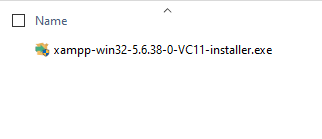
\includegraphics[width=0.50\textwidth]{figures/xampp/hasil.png}}
	\caption{Xampp exe}
	\label{x1}
\end{figure}

\item Kemudian setelah itu jalankan file tersebut dengan cara klik kanan pilih run administrator seperti pada gambar \ref{x2} berikut 

\begin{figure}[!htbp]
	\centerline{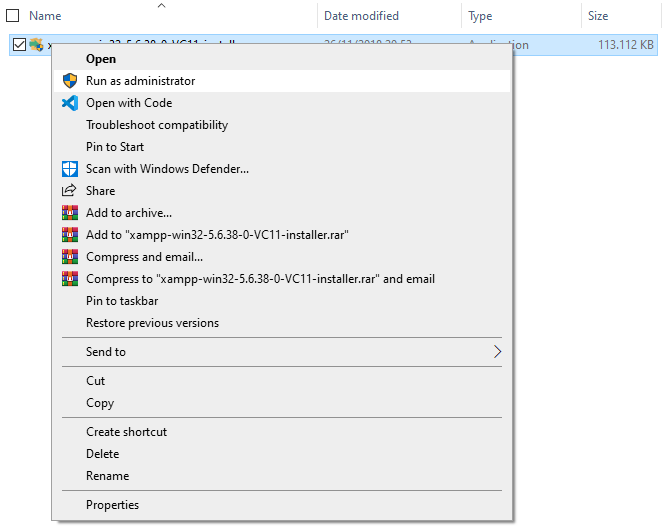
\includegraphics[width=0.60\textwidth]{figures/xampp/1.png}}
	\caption{Run Administrator Xampp}
	\label{x2}
\end{figure}
\pagebreak

\item Kemudan jika muncul popup pilihan untuk memasang aplikasi pada komputer pilih yes, lalu tunggu beberapa saat maka akan muncul setup XAMPP separti pada gambar \ref{x3}.

\begin{figure}[!htbp]
	\centerline{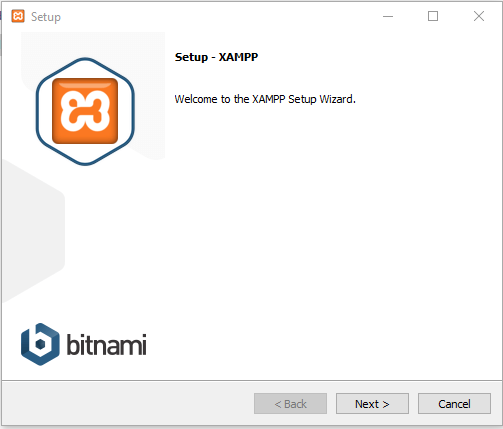
\includegraphics[width=0.70\textwidth]{figures/xampp/2.png}}
	\caption{Setup Xampp}
	\label{x3}
\end{figure}

\item Kemudian klik Next untuk melanjutkan peroses Instalasi \ref{x3}


\begin{figure}[!htbp]
	\centerline{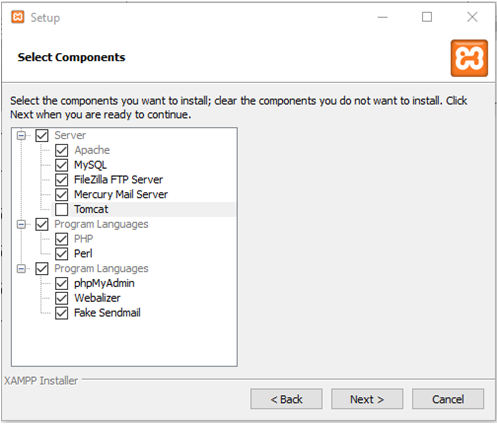
\includegraphics[width=0.70\textwidth]{figures/xampp/3.png}}
	\caption{Memilih Komponen Xampp}
	\label{x4}
\end{figure}

\item Pada gambar \ref{x4} merupakan peroses memilih software yang akan di pasang pada komputer sebagai contoh hilangkan tanda checklist pada check box Tomcat, kemudian kelik tombol Next.

\begin{figure}[!htbp]
	\centerline{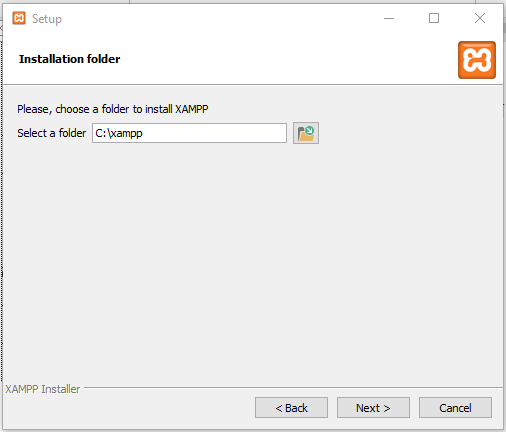
\includegraphics[width=0.70\textwidth]{figures/xampp/4.png}}
	\caption{Tempat Istall Xampp}
	\label{x5}
\end{figure}


\item Pada gambar \ref{x5} merupakan menentukan tujuan instalasi XAMPP, secara default xampp akan teristal pada direktori C:xampp, jika tidak akan menginstall di direktori C maka datapat memilih direktori lain dengan cara klik tmbol browser yang bergambar folder dengan anak panah. Kemudian klik tombol Next untuk melanjutkan peroses.
\pagebreak
\begin{figure}[!htbp]
	\centerline{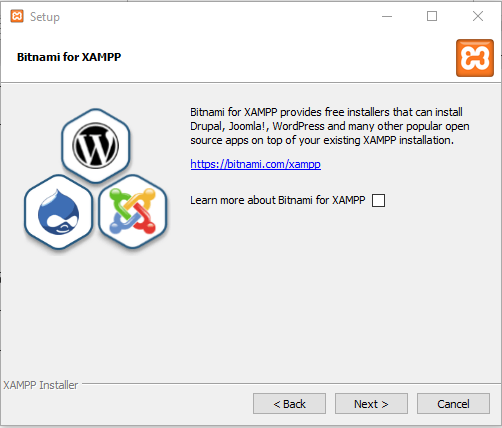
\includegraphics[width=0.70\textwidth]{figures/xampp/5.png}}
	\caption{Bitami Untuk Xampp}
	\label{x6}
\end{figure}


\item Pada gambar \ref{x6} uncheck checklist yang terdapat pada halaman tersebut, kemudian klik tombo Next untuk melanjutkan peroses installasi.
 
\begin{figure}[!htbp]
	\centerline{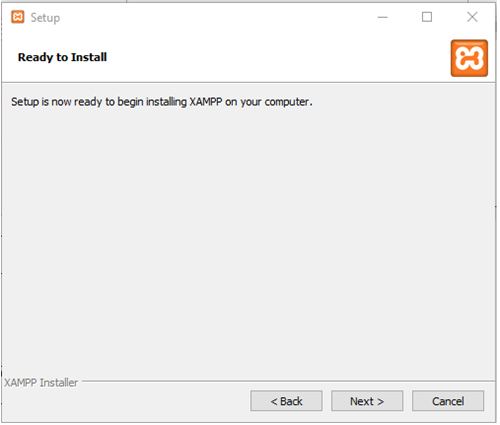
\includegraphics[width=0.70\textwidth]{figures/xampp/6.png}}
	\caption{Xampp Siap diinstal}
	\label{x7}
\end{figure}
 
\item Pada gambar \ref{x7} menunjukan bahwa semua aplikasi yang telah di cheklis tadi dan telah di tentukan tempat installnya, telah siap untuk diinstal, kemudian klik tombol Next untuk melanjutkan proses instal
 


\item Pada gambar \ref{x8} menunjukan peroses install aplikasi pada peroses ini tunggu instal aplikasinya beres jika muncul popup klik finish untuk mengakhiri proses istalasi
\begin{figure}[!htbp]
	\centerline{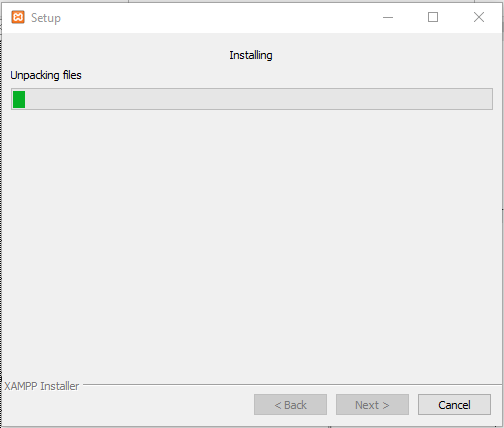
\includegraphics[width=0.70\textwidth]{figures/xampp/7.png}}
	\caption{Proses Install Xampp}
	\label{x8}
\end{figure}

\item pada gambar \ref{x9} tersebut kemudian klik tombol open untuk memunculkan XAMPP control panel
\begin{figure}[!htbp]
	\centerline{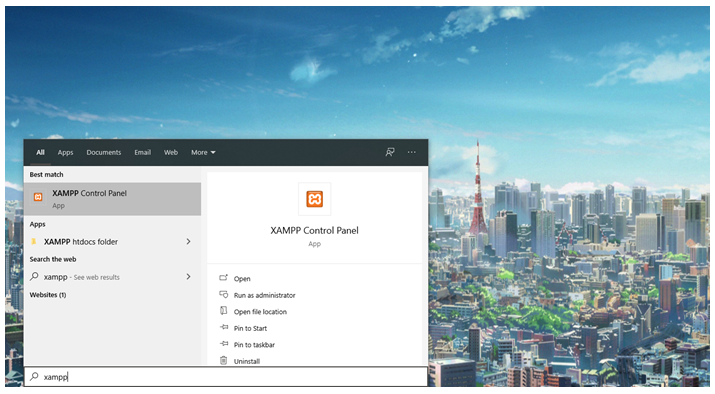
\includegraphics[width=1\textwidth]{figures/xampp/8.png}}
	\caption{Membuaka Xampp}
	\label{x9}
\end{figure}

\item pada gambar \ref{x10} tersebut jalankan service apache dan MySQL dengan cara klik tombol start yang terdapat di sebelah tulisan apache dan MySQL.
\begin{figure}[!htbp]
	\centerline{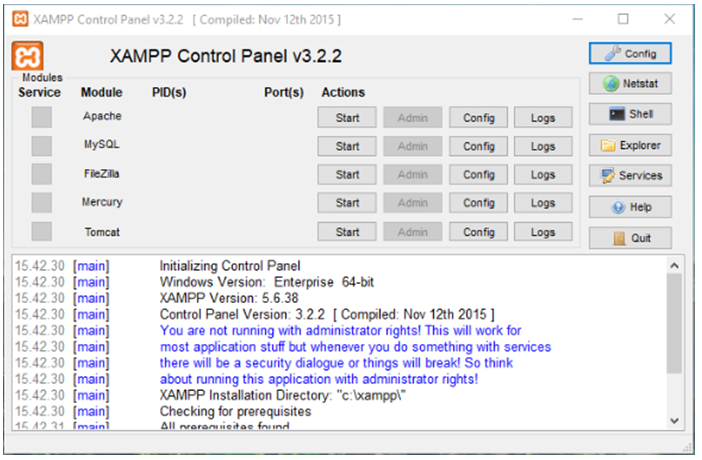
\includegraphics[width=1\textwidth]{figures/xampp/9.png}}
	\caption{Control Panel Xampp}
	\label{x10}
\end{figure}
\end{enumerate}
\textbf{Catatan :}\par
\textit{Untuk melatekan dokumen codeigniter pada xampp dapat di simpan pada dokumen root apache yang terletak pada Direktori C pada folder xampp di subfolder htdocs }\pagebreak


%% editor teks 
\section{ Editor Text yang Digunakan}
	Setelah xampp terinstall, maka selanjutnya di butuhkan editor text yang digunakan untuk membuat souce code atau kode baik itu php, html, java script dan lainnya, untuk editor text itu sendiri banyak ragamnya seperti notepad++, SublimeText 3, atom dan lain-lain, terkhusus pada buku ini untuk tolls editor teksnya menggunakan visual studio code yang merupakan editorteks yang di liris oleh  microsoft dan editor teks ini gratis.

\subsection{Kelebihan dari Visual Studio Code}
Adapun kelebihan dari editor teks visual studio code yaitu:
\begin{enumerate}
\item dapat di gunakan pada semua sistem operasi yaitu windows, linux, dan macos
\item banyak menyediakan ekstensi sehingga mempermudah dalam melakukan pembuatan kode
\item dapat terintegrasi dengan git 
\item dapat membuka terminal atau comand from pada aplikasi visual studio code
\end{enumerate}

\subsection{Instalasi Visual Studio Code}
	pada peroses instalasi visual studio code dilakukan untuk sistem operasi windows, kemudian untuk menerapkan visual studio code pada sistem operasi windows dapat mengikuti tahapan-tahapan seperti berikut:
\begin{enumerate}
\item Unduh terlebih dahulu visual studio code pada website resminya pada alamat berikut https://code.visualstudio.com/ untuk halaman utama website tersebut seperti pada gambar \ref{V1} berikut:\par
 \begin{figure}[!htbp]
	\centerline{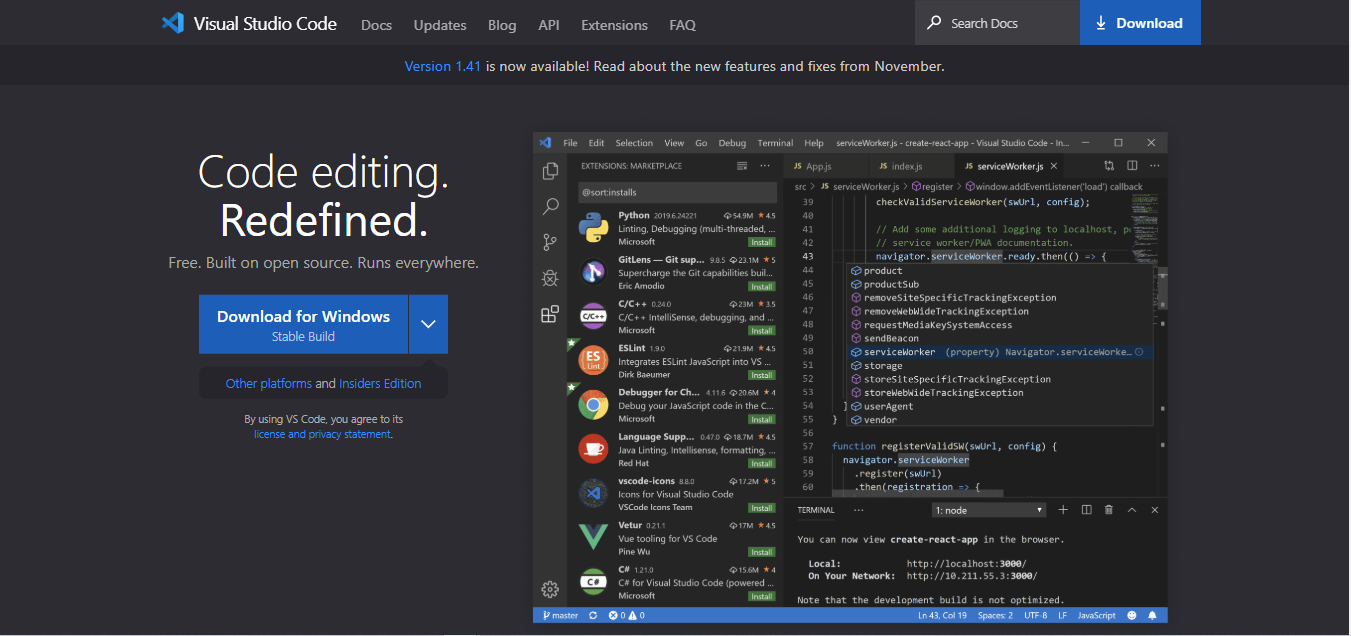
\includegraphics[width=0.90\textwidth]{figures/vs/1.png}}
	\caption{Halaman Utama Website Visual Studio Code}
	\label{V1}
\end{figure}
\item jika telah muncul tampilan seperti gambar \ref{V1} pilih tombol download for windows yang terdapat pada sebelah kiri halaman tersebut, jika yang munculnya bukan pilihan download for windows bisa dicari dengancara menekan tombol panah yang terdapat disebelah tombol download forwindows, hal ini juga bisa dilakukan jika ingin mengunduh visual studio code untuk sistem oprasi linux atau mac, untuk detail pilihan untuk opsi download seperti pada gambar \ref{V2}.\par

\begin{figure}[!htbp]
	\centerline{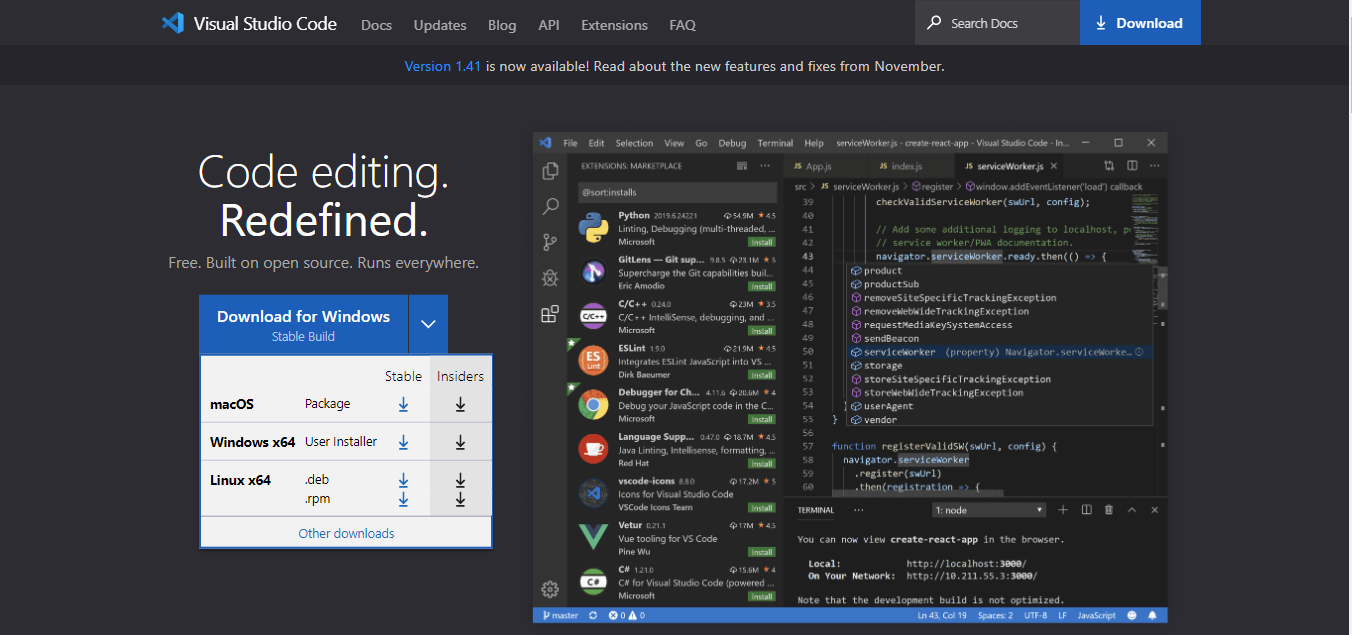
\includegraphics[width=0.9\textwidth]{figures/vs/2.png}}
	\caption{Memilih Visial Studio Berdasarkan OS}
	\label{V2}
\end{figure}
 
\item dikarenakan pada projek yang akan di bahas pada buku ini menggunakan sistem operasi windows sehingga pada tampilan di gambar \ref{V2} pilih visual studio for windows kemudian unduh file tersebut\par 

\begin{figure}[!htbp]
	\centerline{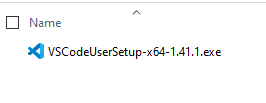
\includegraphics[width=0.6\textwidth]{figures/vs/3.png}}
	\caption{File exe visual studio code}
	\label{V3}
\end{figure}

\item Jika sudah di unduh maka hasil unduhnya berupa file exe seperti pada gambar \ref{V3} dimana file tersebut akan di jalankan agar visual studio dapat di terapkan pada komputer atau laptop yang akan di gunakan untuk pemerograman.\par

\item Pada Gambar \ref{V4} merupakan peroses awal untuk instalasi visual code dengan cara klik kanan pilih Run as administrator atau degan cara klik duakali pada file visual studio code lalu tngggu beberapa saat, jika munul notifikasi berupa pop up klarifikasi untuk install aplikasi, pilih yes untuk melanjutkan proses.\par \pagebreak
\begin{figure}[!htbp]
	\centerline{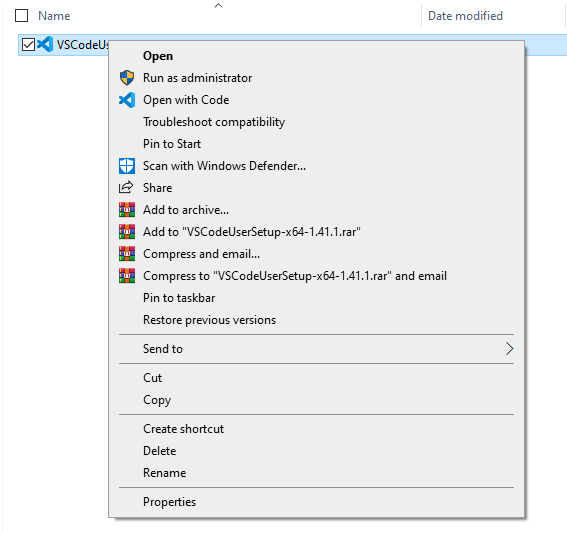
\includegraphics[width=0.6\textwidth]{figures/vs/4.png}}
	\caption{Run Administrator}
	\label{V4}
\end{figure}

\item Pada gambar \ref{V5} merupakan pilihan lisensi atau ketentuandari visual studio code, pada tampilan ini pilih I accept the agreement yang merupakan perintah bahwa menyetujui ketentuan yang di berikan untuk pemasangan aplikasi visual studio code setelah itu klik tombol Next, untuk melanjutkan peroses instalasi.
 \begin{figure}[!htbp]
	\centerline{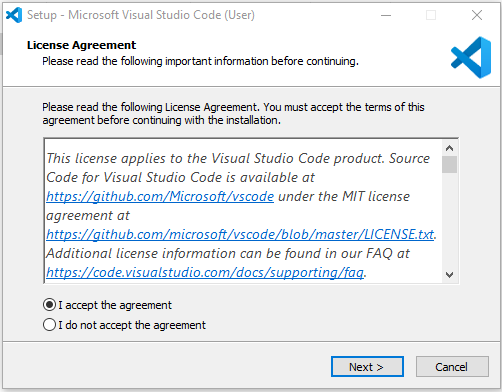
\includegraphics[width=0.80\textwidth]{figures/vs/5.png}}
	\caption{Persetujuan Lisensi}
	\label{V5}
\end{figure}

\item Pada gambar \ref{V6}  merupakan opsi untuk tempat di installnya aplikasi visual studio code secara default visual studio code akan terinstal di direktori 
\begin{verbatim} C:\User\nama_user\AppData\Local\Programs
\Microsoft VS Code 
\end{verbatim}
 jika ingin memilih opsi lain dapat memilih tombol Browse… kemudian memilih folder tempat di installnya visual studio code, jika telah selesai klik tombol Next untuk melanjutkan proses install
\begin{figure}[!htbp]
	\centerline{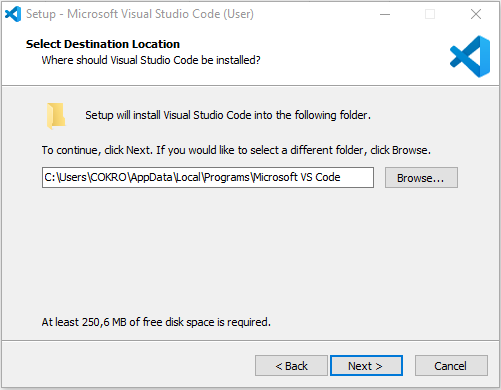
\includegraphics[width=0.90\textwidth]{figures/vs/6.png}}
	\caption{Direktori Visual Code Di install}
	\label{V6}
\end{figure}
 \pagebreak
\item Pada gambar \ref{V7} merupakan opsi untuk memilih start menu, jika telah memilih start menu maka klik Next untuk melanjutkan proses install

\begin{figure}[!htbp]
	\centerline{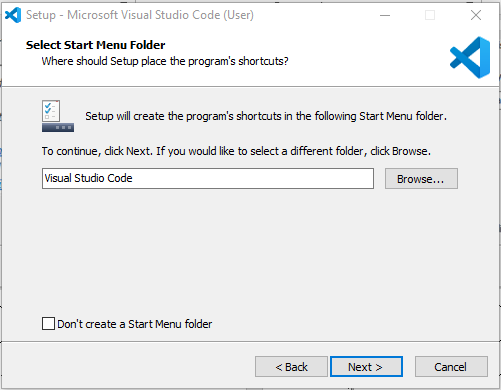
\includegraphics[width=0.90\textwidth]{figures/vs/7.png}}
	\caption{Memilih Start Menu}
	\label{V7}
\end{figure}
\item Pada gambar \ref{V8}  merupakan opsi untuk menembahkan taks, dengan di tambahkannya taks maka untuk membuka file pemerograman bisa dengan klik kanan pada file pemerograman kemudian open with visual code, tidak hanaya itu dengan di ceklisnya taks pada pilihan tersebut file yang berekstensi php,html, dan lainnya yang berekstensi kode pemerograman akan memiliki icon sesuai dengan ekstensi dari file tersebut, kemudian pada taks PATH agar visual code bisa mengakses comand from atau terminal, untuk rekomendasi taks yang harus di pilih dapat dilihat pada gambar \ref{V8}. jika suadah dipilih sesuai dengan gambar maka bisa dilanjutkan dengan menekan atau klik tombol Next, untuk melanjutkan proses istall visual code.
 \pagebreak
\begin{figure}[!htbp]
	\centerline{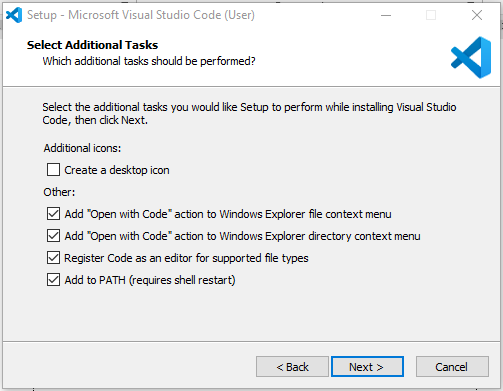
\includegraphics[width=0.80\textwidth]{figures/vs/8.png}}
	\caption{Menambahkan Taks}
	\label{V8}
\end{figure}

\begin{figure}[!htbp]
	\centerline{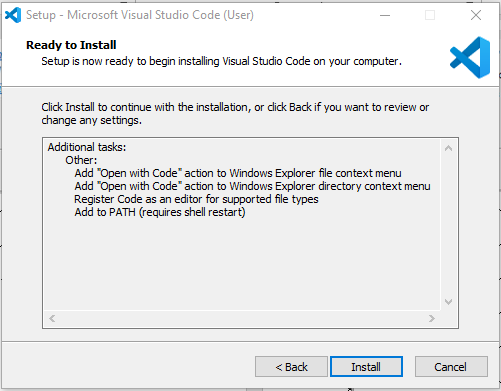
\includegraphics[width=0.80\textwidth]{figures/vs/9.png}}
	\caption{Visual Studio Siap Di Install}
	\label{V9}
\end{figure}

\item Kemudian Pada gambar \ref{V9} menunjukan bahwa visual studio code telah siap untuk di install, klik Install untuk melanjutkan proses install visual studio code. 



\item Pada gambar \ref{V10} merupakan peroses install aplikasi, pada proses ini tunggu sekitar 5 menit jika telah selesai maka akan muncul gambar seperti pada gambar \ref{V10} berikut.

\begin{figure}[!htbp]
	\centerline{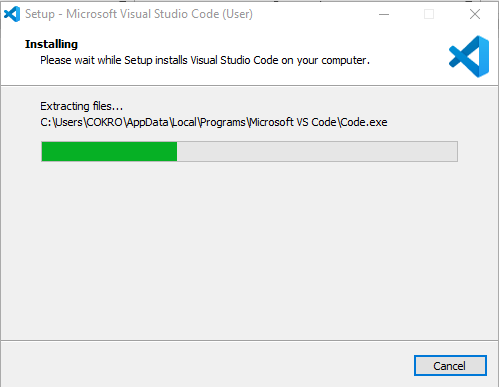
\includegraphics[width=0.70\textwidth]{figures/vs/10.png}}
	\caption{Proses Install Visual Code}
	\label{V10}
\end{figure}

\item Setelah muncul seperti gambar \ref{V11} kemudian klik finish untuk mengakhiri proses instalasi visual studio code. 
\begin{figure}[!htbp]
	\centerline{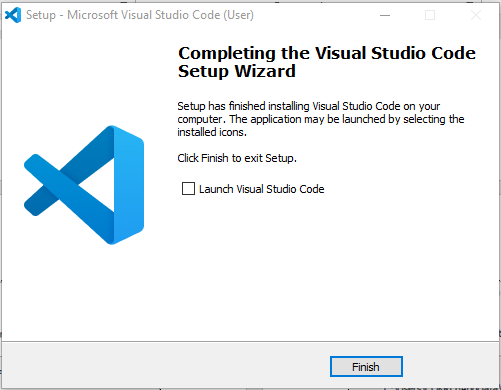
\includegraphics[width=0.70\textwidth]{figures/vs/11.png}}
	\caption{Visual Studio Selesai Di Install}
	\label{V11}
\end{figure}
 
\item Untuk dapat menjalankan visual studio code dapat dengan cara klik icon search yang berada di dekat icon vindows yang berada pada task bar kemudian tekan dan ketik visual maka muncul visual tudio code dan klik open untuk menjalankan visual studio code untuk jelasnya seperti pada gambar \ref{V12}. 

\begin{figure}[!htbp]
	\centerline{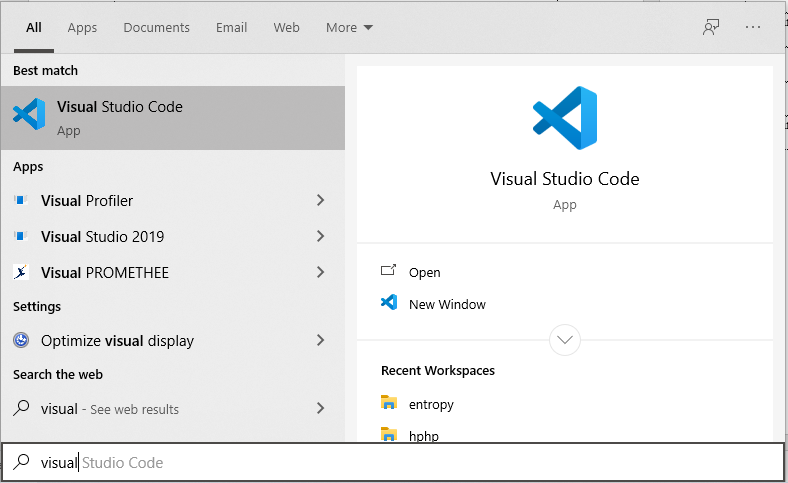
\includegraphics[width=0.90\textwidth]{figures/vs/12.png}}
	\caption{Mencari Visual Studio}
	\label{V12}
\end{figure}


\item Pada gambar \ref{V13} merupakan tampilan awal visual studio code jika telah selesai di install.
\begin{figure}[!htbp]
	\centerline{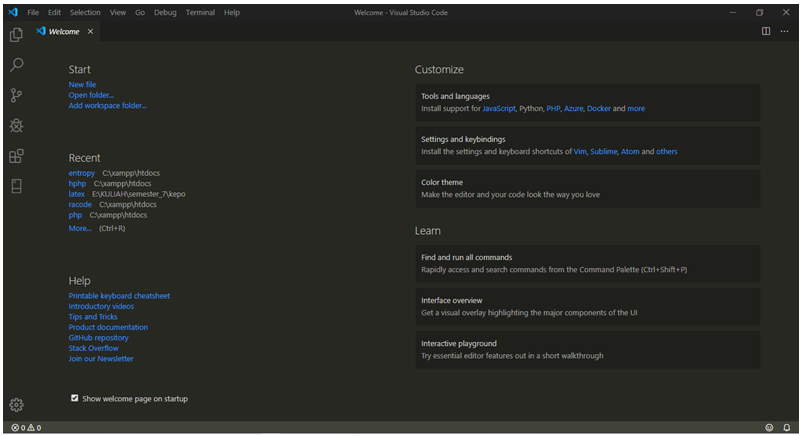
\includegraphics[width=0.90\textwidth]{figures/vs/13.png}}
	\caption{Tampilan Awal Visual Studio}
	\label{V13}
\end{figure}

\item Pada gambar \ref{V14}  merupakan menu untuk memilih ekstensi yang dapat di terapkan pada visual studio code.\par
\begin{figure}[!htbp]
	\centerline{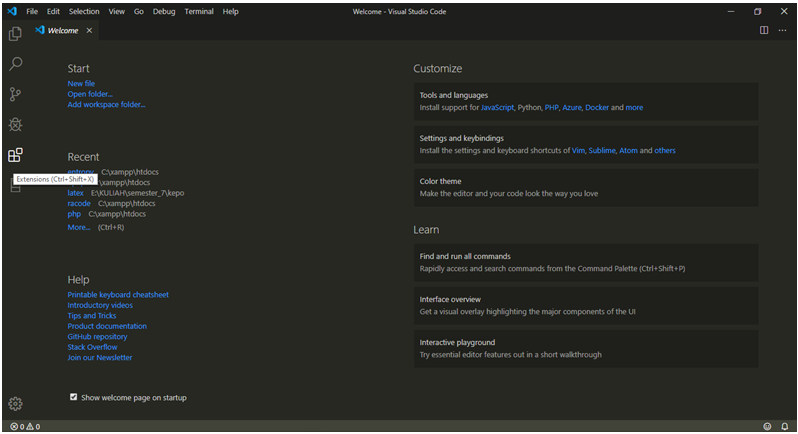
\includegraphics[width=0.90\textwidth]{figures/vs/14.png}}
	\caption{Menu Ekstensi Visual Studio}
	\label{V14}
\end{figure}
\pagebreak

\end{enumerate}


\subsection{Ekstensi Visual Studio Code}

Ekstensi merupakan tolls tambahan yang di gunakan pada aplikasi, adapun pada visual studio code ekstensi yang di gunakan merupakan tambahan tolls untuk membantu dalam pembuatan souce code, dengan di tambahkannya ekstensi pada visual studio code maka dalam pembuatan source code menjadi lebih cepat dan mudah, dikarenakan dengan di tambahkannya ekstensi source code yang error dapat terdeteksi kemudian jika kita akan menulis suatu code hanya perlu menuliskan dua atau tiga huruf pertama kemudian dengan ekstensi tersebut akan di rekomendasikan code yang akan di gunakan. maka dari itu pada buku ini projek yang di buat menggunakan teks editor visual studio code, adapun tambahan ekstensi yang di gunakan agar menunjang projek yang dilakukan pada buku ini adalah sebagai berikut:
\begin{enumerate}
\item Auto Rename Tag\par
Digunakan untuk merename atau mengganti nama tag pembuka dan penutup secara bersamaan, digunakan untuk HTML dan CSS 
Contoh untuk mengganti nama dari 
\begin{verbatim}
<div> … </div>
\end{verbatim}
 menjadi 
\begin{verbatim}
<td>…</td>
\end{verbatim}
maka dengan menggunakan ekstensi tersebut tidak perlu khawatir ada tag dari souce code yang salah di ganti atau di edit.
\pagebreak
\item Indent-rainbow\par
Untuk memberi tanda garis berupa warna, sehingga dapat di ketahui tag pembuka dan tag penutup dari suatu source code. Contoh seperti pada gambar \ref{V15} berikut.

\begin{figure}[!htbp]
	\centerline{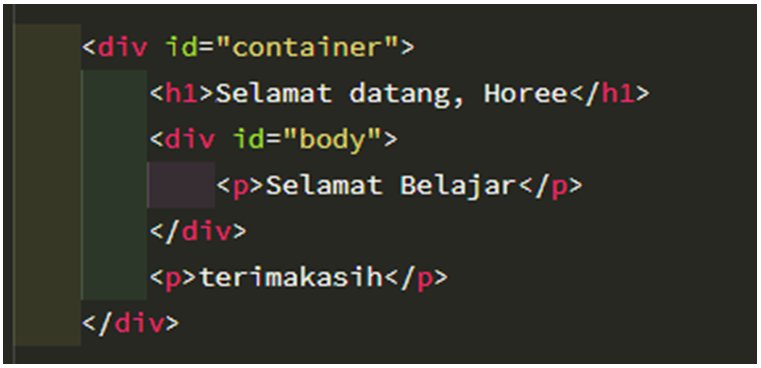
\includegraphics[width=0.80\textwidth]{figures/vs/15.png}}
	\caption{Contoh Penggunaan Indent-rainbow}
	\label{V15}
\end{figure}

pada gambar \ref{V15} tersebut merupakan source code CSS, dimana pada tag pembuka div pertama dapat di ketahui div penutupnya dengan tanda warna hujau transparan kemudian pada tag div ke dua juga dapat diketahui tag pembuka dan penutupnya melalui tanda warna ungu yang segaris dengan kedua tag tersebut.

\item Beautify\par
Digunakan untuk merapihkan code sehingga menjadi lebih teratur sebagai contoh seperti pada gambar \ref{V16} untuk source code yang tidak rapih sehingga menghasilkan source code yang rapih seperti pada gambar \ref{V17} 
 

\begin{figure}[!htbp]
	\centerline{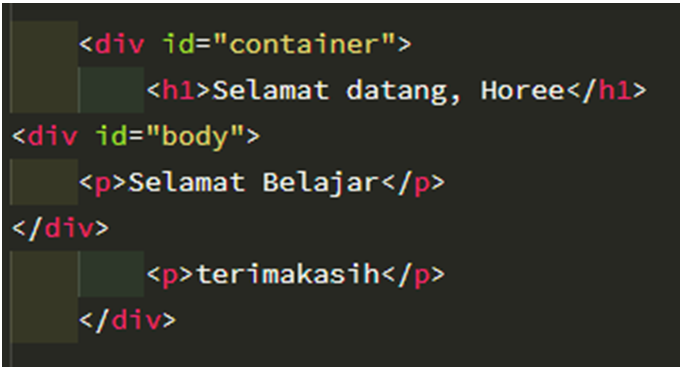
\includegraphics[width=0.90\textwidth]{figures/vs/16.png}}
	\caption{Souce code Acak}
	\label{V16}
\end{figure}

\begin{figure}[!htbp]
	\centerline{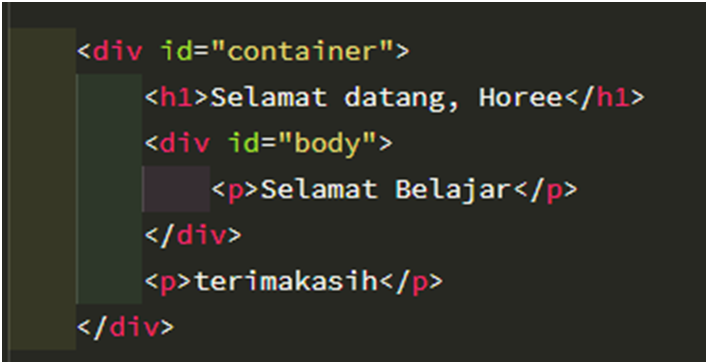
\includegraphics[width=0.90\textwidth]{figures/vs/17.png}}
	\caption{Source Code Rapih}
	\label{V17}
\end{figure}

berdasarkan pada gambar \ref{V16} dan gambar \ref{V17} untuk mengaktifkan ekstensi Beautify bisa di jalankan dengan cara menekan tombol ctrl dan S maka source code yang awalnya tidak beraturan akan menjadi rapih dan lebih tertata.


\item IntelliSense for CSS class names HTML\par
digunakan untuk mengkoreksi tag-tag dari CSS dan HTML, selain untuk mengkoreksi juga di gunakan untuk merekomendasikan Source code yang akan digunakan atau tag yang akan di gunakan. Misalkan progrmer akan menuliskan tag html, dengan menggunakan ekstensi tersebut cukup menuliskan tiga hurup tag pertama seperti <ht maka akan muncul rekomendasi tag html, jika telah muncul kemudian tekan enter maka secara otomatis tag pembuka dan penutup html jadi.
\item Material Icon Theme\par
Digunakan untuk memberikan icon pada folder atau file sesuai dengan fungsinya masing-masing misalkan seperti file php maka akan ada icon php begitupula file html maka akan memiliki icon html, agar lebih jelas maka hasilnya seperti pada gambar \ref{V18} berikut:
\begin{figure}[!htbp]
	\centerline{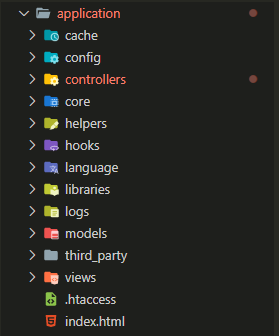
\includegraphics[width=0.45\textwidth]{figures/vs/18.png}}
	\caption{Menu Ekstensi Visual Studio}
	\label{V18}
\end{figure}
\item Monokai Theme\par
Merupakan ekstensi yang digunakan untuk merubah tema atau tampilan dari visual studio code, tampilan visual studio code jika menggunakan ekstensi ini akan seperti sublime text 3 dari tulisan hingga pewarnaan setiap tag source code,Bagi yang biasa menggunakan teks editor sublime text 3 dianjurkan untuk menggunakan ekstensi ini agar tampilan code menjadi seperti sublime text 3, sehingga menjadi pamiliar dan mempermudah dalam membuat sourcecode.

\pagebreak
\item PHP intellisense for codeigniter\par
Digunakan untuk mengkoreksi atau secara otomatis merekomendasikan code yang akan ditulis sesuai dengan librari codeigniter, misalkan menuliskan \$this-  maka akan ada rekomendasi tag penerusnya seperti input atau yang sejenisnya atau juga ketika memanggil sebuah model maka setelah menulis class model maka akan muncul rekomendasi fungsi-fungsi yang terdapat pada class pada model tersebut atau kasus lan seperti pada saat menuliskan ekstensi pada class maka akan muncul rekomendasi library yang akan di gunakan.\par


Sebagai alternatif untuk menerapkan ekstensi pada visual studio code bisa dengan cara memasukan source code tersebut pada settings.json yang terdapat  pada visual studio code, untuk lebih jelasnya berikut merupakan code yang harus di sesuaikan pada settings.json.

\end{enumerate}
\begin{lstlisting}[language=php]
{
    "workbench.colorTheme": "Monokai",
    "workbench.iconTheme": "material-icon-theme",
    "explorer.openEditors.visible": 0,
    "editor.minimap.enabled": false,
    "editor.lineHeight": 23,
    "editor.fontFamily": "'Source Code Pro',Consolas, 'Courier New', monospace",
    "terminal.integrated.shell.windows": "C:\\WINDOWS\\System32\\WindowsPowerShell\\v1.0\\powershell.exe",
    "php.suggest.basic": false,
    "editor.formatOnSave": true,
    "liveServer.settings.donotShowInfoMsg": true,
    "files.autoSave": "afterDelay"
}
\end{lstlisting} 

\section{ Instalasi \textit{CodeIgniter}}

Framework code igniter dapat di unduh website resminya yaitu www.codeigniter.com untuk tampilannya seperti pada gambar \ref{C1} beriku:\par
\begin{figure}[!htbp]
	\centerline{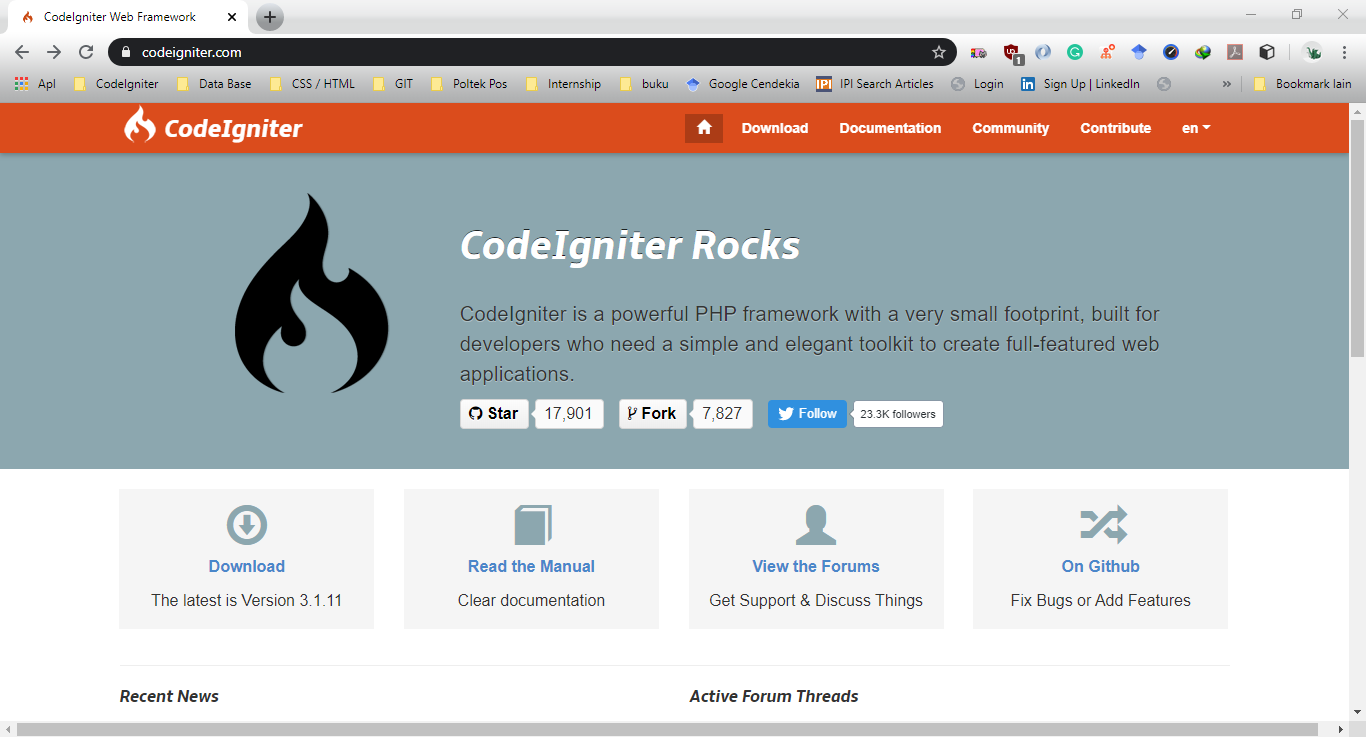
\includegraphics[width=1\textwidth]{figures/ci/1.png}}
	\caption{Tampilan Website CodeIgniter}
	\label{C1}
\end{figure}
Pada buku ini akan mengunakan codeigniter versi 3.1.11 yang terbaru pada saat buku ini di tulis. Untuk dapat mengunduhnya dapat menekean menu download yang terdapat pada halaman utama web resmi codeigniter atau dengan cara menekan menu download yang terdapat pada navigator bar maka akan pindah halaman ke halaman download pada halaman tersebut pilih menu codeigniter 3 dan download seperti pada gambar \ref{C2},
\begin{figure}[!htbp]
	\centerline{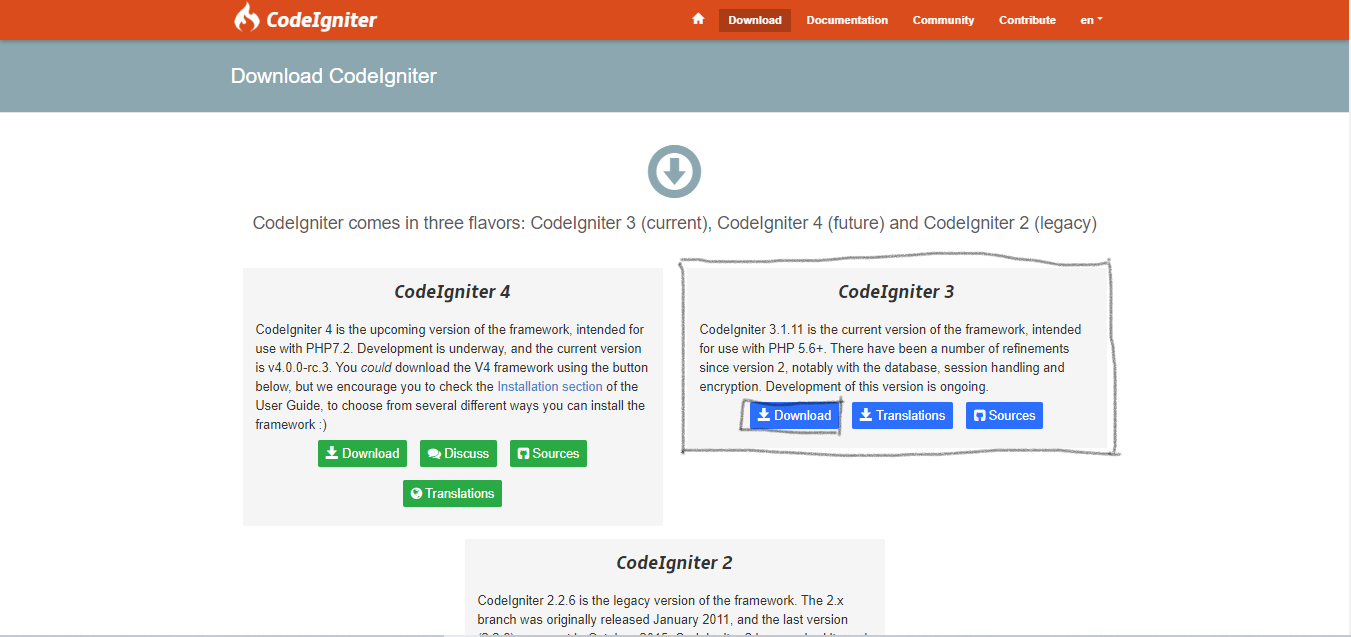
\includegraphics[width=1\textwidth]{figures/ci/2.png}}
	\caption{Halaman Download CodeIgniter}
	\label{C2}
\end{figure}
Setelah di unduh maka hasil file nya berupa zip dapat dilihat pada gambar \ref{C3}, setelah itu ekstrak file zip tersebut kemudian pindahkan ke direktori \begin{verbatim} C:\xampp\htdocs\end{verbatim} lalu agar mempermudah pemanggilan terhadap folder codeigniter bisa dilakukan dengancara mengganti nama folder codeigniter sebut misalkan menjadi CI sehingga hasilnya seperti pada gambar \ref{C4}.\par
\begin{figure}[!htbp]
	\centerline{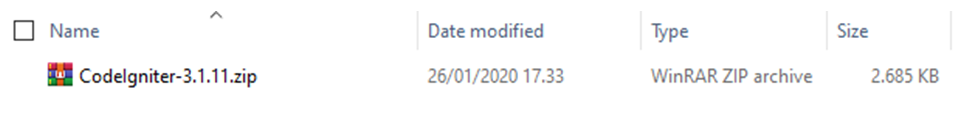
\includegraphics[width=1\textwidth]{figures/ci/3.png}}
	\caption{Hasil download file codeigniter}
	\label{C3}
\end{figure}
\begin{figure}[!htbp]
	\centerline{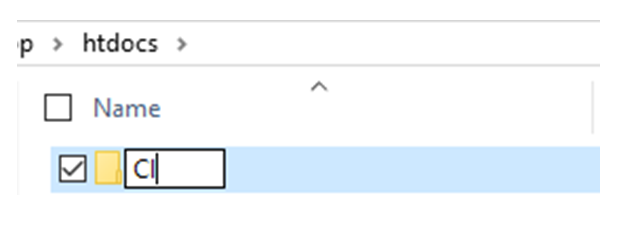
\includegraphics[width=0.85\textwidth]{figures/ci/4.png}}
	\caption{Folder CodeIgniter yang telah di rename}
	\label{C4}
\end{figure}
\pagebreak
Kemudian untuk memeriksa apakah codeigniter telah tepasang dengan benar atau belum dapat dilakukan dengan cara menuliskan alamat berikut :
 \begin{verbatim} http://localhost/CI \end{verbatim}

pada web browser yang di gunakan, jika codeignite rberjalan dengan baik maka hasilnya akan sepert pada gambar \ref{C5} berikut:
\begin{figure}[!htbp]
	\centerline{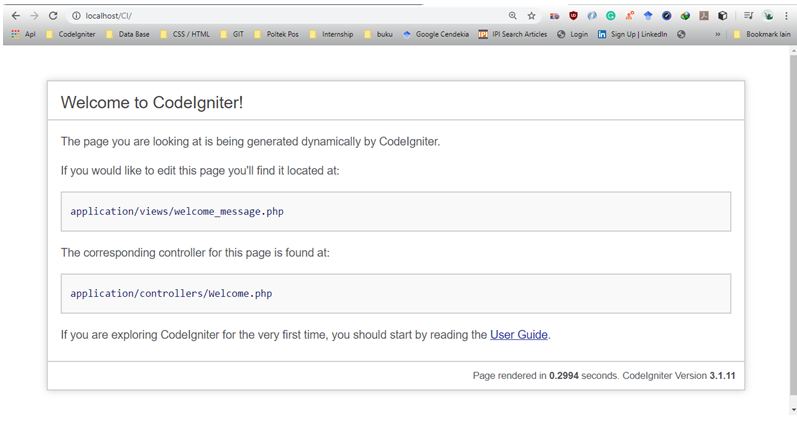
\includegraphics[width=1\textwidth]{figures/ci/5.png}}
	\caption{Hasil CodeIgniter}
	\label{C5}
\end{figure}
\subsection{Desain MVC}

Pada teknik pemerograman berorientasi objek, MVC atau model-view-controller merupakan sebuah metodelogi atau pola desain (desain pattern) yang digunakan untuk merelasikan data dan user interface dari suatu sistem agar menjadi efisien. Awalmulanya MVC digunakan untuk pemerograman berbasis dekstop khususnya untuk aplikasi-aplikasi yang di kembangkan menggunakan bahasa pemerograman C++, Java, dan Smalltalk, dengan semakin berkembangnya teknologi kini pengaplikasian model MVC tersebut diadopsi pada aplikasi yang berbasis web, sehingga hampir semua framework yang di gunakan untuk pengembangan web menggunakan konsep MVC \cite{raharjo2015belajar} .

Adapun komponen pada MVC dibagi menjadi tiga bagian yaitu:
\begin{enumerate}

\item Model yang berfungsi untuk mempresentasikan struktur data
\item View berfungsi untuk epresentasi keluaran atau output dari model yang berkaitan.
\item Controller  yang berpungsi untuk mengambil masukan dari user atau inputan dari user dan mengubahnya menjadi perintah untuk mengeksekusi model dan/atau view

\end{enumerate}

Umunya pola MVC dapat digambarkan seperti pada gambar \ref{C6} berikut :

\begin{figure}[!htbp]
	\centerline{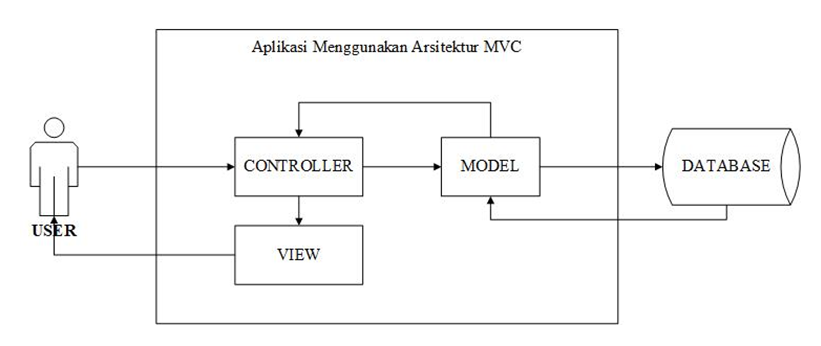
\includegraphics[width=1\textwidth]{figures/ci/6.png}}
	\caption{Alur Pola MVC Pada CodeIgniter}
	\label{C6}
\end{figure}

	pada gambar \ref{C6} tersebut dapat dijelaskan bahwa proses MVC dimulai dari aksi yang diberikan oleh user pengguna sistem kemudian aksi tersebut di terima oleh class dan method atau fungsi yang berangkutan pada controller  kemudian controller mengirim pesan ke model jika pada model tidak bersangkutan dengan basis data maka akan di kembalikan ke controller namun jika pada model bersangkutan dengan basis data maka fungsi pada model yang bersangkutan akan melakukan eksekusi pada data yang terdapat pada database tergantung pada fungsinya kemudian setelah itu data di kembalikan pada controller, kemudian controller menjalankan fungsi yang berkaitan dengan dta tersbut lalu mengirimkan data tersebut pada view yang menjadi user interface kepada user pengguna sistem.
\pagebreak

\subsection{Isi Folder CodeIgniter}

Isi folde atau susunan direktori pada codeigniter, pada satu paket codeigniter yang telah di download di dalammya terdapat tiga folder atau tiga direktori yaitu :
\begin{enumerate}
\item Apllication 
\item System 
\item User guide 
\end{enumerate}
Berikut merupakan penjelasan isi setiap folder yang terdapat pada satu paket codeigniter.


\subsection{Struktur Direktori Pada Folder Apllication}
Direktori application merupakan tempat file-file dari aplikasi yang akan dibuat. Berikut juga model MVC juga terdapat pada direktori ini. Kemudian jika ingin menambahkan fitur-fitur untuk aplikasi juga di simpan pada direktori ini, seperti template css javascrip, template HTML, dan file untuk eksport data, juga harus di simpan pada direktori ini. File-file tersebut di simpan pada folder atau subdirektori yang telah di sediakan oleh codeigniter itu sendiri.
Adapun daftar sub durektori yang terdapat pada direktori apllikasi seperti pada gambar \ref{C7} berikut:
\begin{figure}[!htbp]
	\centerline{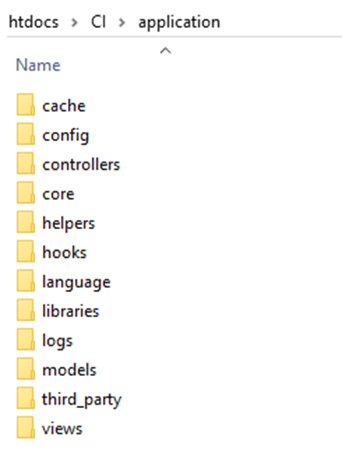
\includegraphics[width=0.40\textwidth]{figures/ci/7.png}}
	\caption{Isi Folder Apllication}
	\label{C7}
\end{figure}

Adapun penjelasan dari direktori pada gambar 16 tersebut sebagai berikut:
\begin{enumerate}
\item chace, digunakan untuk menyimpan halaman-halaman yang telah di buka sebelumnya kemudian di sembunyikan (chaced)
\item	config, berisikan file-file konfigurasi yang digunakan untuk aplikasi yang dibuat.
\item controller, berisi file-file controller dari aplikasi.
\item core, digunakan untuk menempatkan daftar file kelas dasar (base class) yang nantinya diturunkan pada class-class yang digunakan oleh aplikasi 
\item helpers, digunakan untuk menyimpan atau menempatkan file-file helper atau pustaka buatan sendiri yang di definisikan sendiri
\item hooks, berisi file pendukung aplikasi. Sebagai contoh, jika kita ingin memanggil suatu fungsi yang tersimpan di dalam file tertentu sebelum atau sesudah file controller dipanggil, maka dapat menempatkan file yang akan di eksekusi tersebut didalam sub direktori ini 
\item language, dalam direktori ini dapat mendefinisikan nilai konstanta-konstanta tertentu dalam bahasa yang diinginkan.
\item libraries, berisi daftar file library (pustaka dalam bentuk kelas yang di definisikan sendiri)
\item logs, digunakan oleh codeigniter untuk menyimpan logs (catatan) catatan yang secara otomatis ketika terjadi kesalahan.
\item models, berisi daftar file model yang di perlukan oleh aplikasi.
\item third party, digunakan untuk menyimpan plugin yang dikembangkan oleh pihak ketiga.
\item views, berisi file view yang digunakan oleh aplikasi.
\end{enumerate}

	
\subsection{Struktur Direktori Pada Folder System}
Pada direktori ini berisikan file-file yang telah di sediakan oleh codeigniter yang telah di kelasifikasikan berdasarkan fungsinya masing-masing, adapun sub kategori yang berada pada direktori system seperti pada gambar \ref{C8} berikut:

\begin{figure}[!htbp]
	\centerline{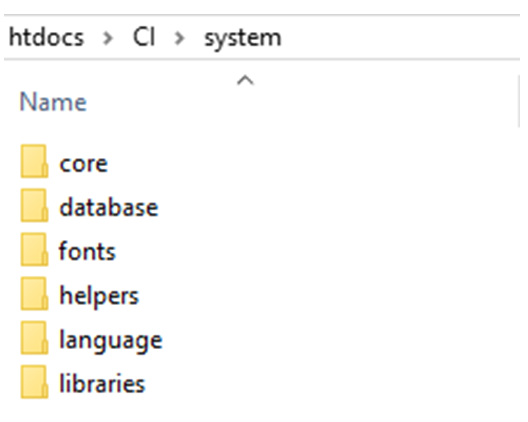
\includegraphics[width=0.40\textwidth]{figures/ci/8.png}}
	\caption{Isi Folder Apllication}
	\label{C8}
\end{figure}

\begin{enumerate}
\item core, berisikan file-file inti berupa class-class yang di gunakan oleh codeigniter, seperti CI\_Controller, CI\_Model dan lain-lain
\item database, berisikan file daftar file driver yang digunakan untuk mengakses database.
\item fonts, berisikan daftar file font 
\item helpers, berisi daftar file helper standar yang di sediakan oleh codeigniter.
\item language, berisi file-file bahasa (untuk keperluan translasi bahasa)
\item libraries, berisi daftar file daftar pustaka kelas standar yang di sediakan oleh codeigniter
\end{enumerate}

\subsection{Direktori user\_guide}
Direktori ini berisikan file-file dokumentasi penggunaan codeigniter dengan format file HTML direktori ini dapat tidakdi ikut sertakan dalam pembuatan aplikasi. Atau di cut keluar dari direktori temapt di codeugniter. Karena direktori ini tidak bepengaruh pada kedua direktori sebelumnya.

\section{Alur Aplikasi \textit{CodeIgniter}}

Adapun alur dari aplikasi yang ditulis menggunakan codeigniter digambarkan seperti pada gambar \ref{C9} berikut:\par
\begin{figure}[!htbp]
	\centerline{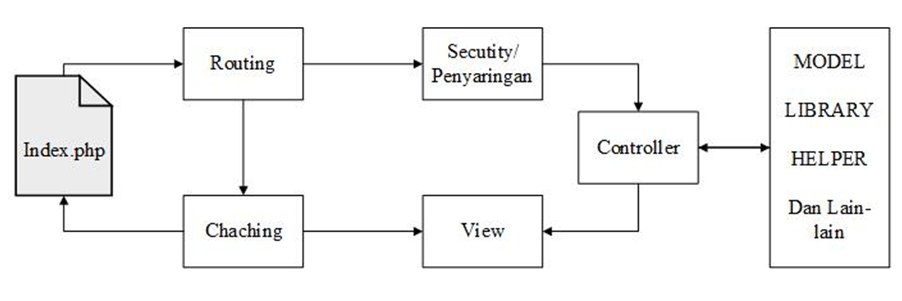
\includegraphics[width=1\textwidth]{figures/ci/9.png}}
	\caption{alur Aplikasi CodeIgniter}
	\label{C9}
\end{figure}

Alur pada gambar \ref{C9} tersebut dapat di jelaskan seperti berikut:
\begin{enumerate}
\item File index.php atau yang sering di sebut dengan entry script berperan sebagai controller depan, yang akan menginisialisasi daftar file yang dibutuhkan untuk menjalankan projek codeigniter. Dimana user melakukan perintah aplikasi ke server web melalui index.php, dengan format Unified Resource Identification (URI) seperti berikut :
\begin{verbatim}http://namahost/index.php/kelas-controller/fungsi  \end{verbatim} 
\item Permintaan yang dikirim oleh user berbentuk URI akan ditangkap oleh router, dan router akan menentukan controller dan metode mana yang harus di panggil
\item Jika ternyata halaman yang diminta oleh user telah di sembunyikan (chaced), halaman tersebut akan diambil dari chace dan langsung di sajikan kedalam web browser.
\item Sebelum controller yang diminta oleh user di eksekusi atau di muat, permintaan tersebut atau semua data yang dikirim oleh user akan di saring terlebih dahulu untuk keperluan pengamanan.
\item Controller akan memeuat model, library, herper, dan file-file yang diperlukan untuk memenuhi permintaaan user
\item Controller akan memuat view untuk di sajikan ke web browser jika mode chacing diaktifkan, maka view akan di caching terlebih dahulu sebelum ditampilkan, dengan demikian jika ada permintaan yang sama maka halaman tersebut tinggal di ambil melalui cache.
\end{enumerate}


\section{ Contoh MVC sederhana}

Aplikasi mengguanakan model MVC merupakan aplikasi yang lengkap, karena pada dasarnya jika menggunakan framework codeigniter maka harus menggunakan model MVC ini, untuk urutan contoh MVC adalah sebagai berikut:
\begin{enumerate}
\item Buat terlebih dahulu model untuk menyajikan data 
\item Buat controller untuk mengambil data dari model dan mengirimkan pada view 
\item Buat view untuk menampilkan data yang telah di kirim oleh controller.
\end{enumerate}
Untuk peroses dalam aplikasi tersebut adalah sebagai berikut:
\begin{enumerate}
\item Controller akan mengambil data yang terdapat pada model.
\item Model mengirimkan data sesuai dengan parameter yang diminta controller, parameter tersebut bisa berupa nama method dan atau variabel yang terdapat pada model
\item Kemudian pada controller ada perintah untuk menampilkan view dimana pada view tersebut akan mengambil data dari controller yang telah diambil dari model, dalam mengambil data biasanya dari controller di kirim menggunakan array assosiatif.
\item Maka view akan memperoses data yang di kirimkan oleh controller sehinga dapat di tampilkan hasil keluarannya sesuai dengan parameter yang digunakan pada controller.
\item Terakhir controller akan memperoses hasil yang ditampilkan oleh view ke layar web browser.
\end{enumerate}
Agar dapat memulai contoh MVC pada codeigniter buka folder codeigniter mengguanakan visual studio code seperti pada gambar \ref{mvc1} berikut:

\begin{figure}[!htbp]
	\centerline{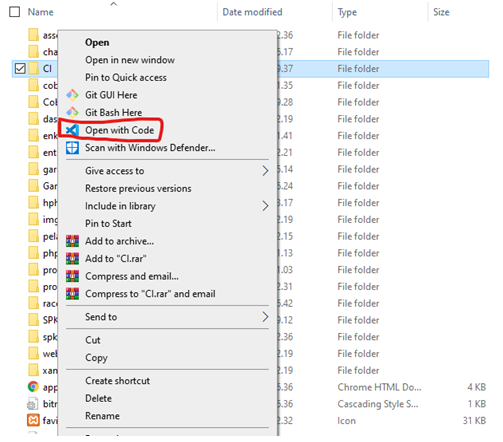
\includegraphics[width=0.80\textwidth]{figures/MVC/1.png}}
	\caption{Open With Visual Code}
	\label{mvc1}
\end{figure}
\pagebreak
%ada gambar

Pada gambar \ref{mvc1} merupakan cara untuk membuka folder codeigniter menggunakan visual studio code untuk hasilnya seperti pada gambar \ref{mvc2} berikut:

\begin{figure}[h]
	\centerline{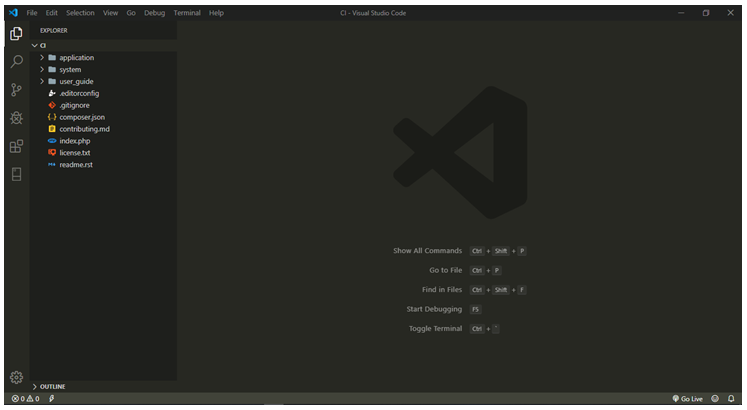
\includegraphics[width=0.95\textwidth]{figures/MVC/2.png}}
	\caption{Folder CodeIgniter Menggunakan}
	\label{mvc2}
\end{figure}
%ada gambar

Pada gambar \ref{mvc2} tampilan direktori code yang di buka menggunakan visual studio code. Setelah tampilannnya seperti pada gambar \ref{mvc2} klik direktori application kemudian pilih sub direktori model sehingga tampilannya seperti pada gambar \ref{mvc3}

\begin{figure}[h]
	\centerline{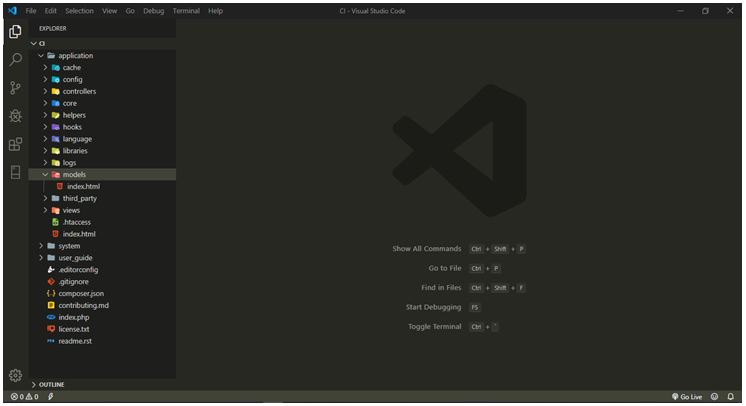
\includegraphics[width=0.95\textwidth]{figures/MVC/3.png}}
	\caption{Direktori Applications}
	\label{mvc3}
\end{figure}
\pagebreak
%ada gambar

Setelah muncul seperti pada gambar \ref{mvc3} kemudian  klik kanan pada sub direktori models kemudian pilih new file dan beri nama model\_mvc.php sehingga hasilnya seperti pada gambar \ref{mvc4} berikut.
\begin{figure}[h]
	\centerline{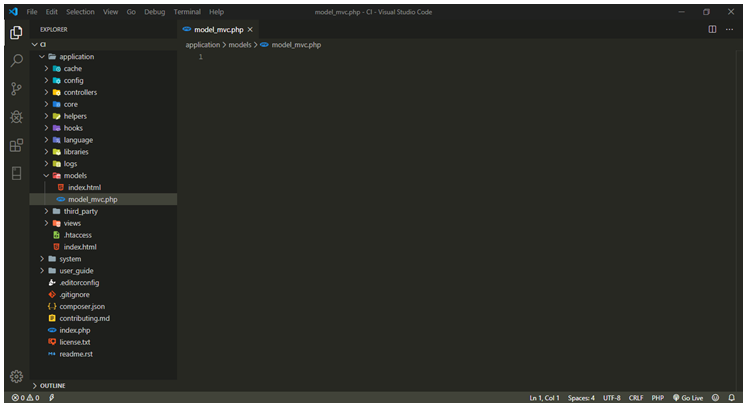
\includegraphics[width=0.95\textwidth]{figures/MVC/4.png}}
	\caption{Membuat File Mode\_mvc}
	\label{mvc4}
\end{figure}
%ada gambar

Jika telah muncul tampilan seperti pada gambar 39 maka masukan codingan berikut pada file model\_mvc.php

\begin{lstlisting}[language=PHP]
<?php
class Model_mvc extends CI_Model
{
    // membuat variabel atau properti dengan nama $str dengan tipe data string
    public $str = 'Mencoba CodeIgniter';
}

\end{lstlisting} 
\textbf{Penjelasan \textit{Source Code}}.\par
	Untuk membuat model hal seperti kode diatas yaitu:
\begin{enumerate}
\item buat tag php pada baris pertama, hal ini dilakukan karena base dari Codeigniter sendiri merupakan PHP
\item pada baris ke dua buat class dengan nama class yang harus sama dengan nama file model hanya hanyasaja pada hurup pertama harus kapital, jika nama filenya \textbf{model\_mvc.php} berarti nama kelasnnya harus \textbf{Model\_mvc}, kemudian harus eksten ke class CI\_Model dikarenakan source code tersebut merupakn model.
\item untuk isi source code pada class tersebut harus di tempatkan di dalam kurung kurawal yang terdapat pada baris ke tiga dan enam pada source code tersebut.
\item pada baris ke empat merupakan comment pada source code tanda coment itu sendiri yaitu garis miring duakali sebelum source code, lalu comment ini tidak akan di tampilkan atau di eksekusi oleh sistem.
\item pada baris ke 5 merupakan variabel atau properti yang berisikan data string kemudian berstatus public yang berarti variabel tersebut bisa di akses oleh class lain.
\end{enumerate}

Setelah memasukan codingan tersebut buat Controller dengan nama Controller\_mvc.php dengan cara klik kanan sub direktori controllers kemudian buat file baru dengan memilih new file kemudian berinama Controller\_mvc.php. maka hasilnya seperti pada gambar \ref{mvc5} berikut

\begin{figure}[h]
	\centerline{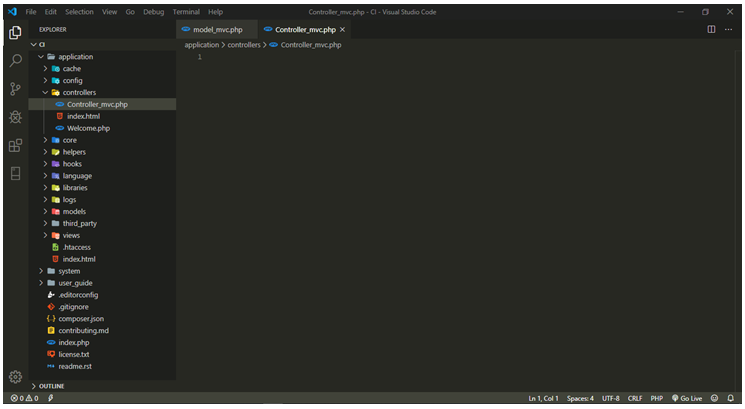
\includegraphics[width=0.95\textwidth]{figures/MVC/5.png}}
	\caption{Membuat File Controller\_mvc}
	\label{mvc5}
\end{figure}

%ada gambar

Jika telah muncul tampilan seperti pada gambar \ref{mvc5} maka masukan codingan berikut pada file Controller\_mvc.php
\begin{lstlisting}[language=PHP]
<?php
class Controller_mvc extends CI_Controller
{
    public function index()
    {
        // memanggil atau memuat 'model_mvc'
        $this->load->model('model_mvc');
        // mengambil objek dari krlas model_mvc'
        // yang dimasukan ke variabel $data_model
        $data_model = $this->model_mvc;
        // mengambil data yang terdapat pada model
        $string = $data_model->str;
        // membuat inisial data yang di kirim ke view
        $data['data'] = $string;
        // menampilakan dan mengirimkan data ke view
        $this->load->view('view_mvc', $data);
    }
}

\end{lstlisting} 
\pagebreak
\textbf{Penjelasan \textit{Source Code}}.\par
	pada dasarnya pembuatan file dan source code pada controller hampir mirip dangan model, untuk penjelasan source code tersebut sebagai berikut:
\begin{enumerate}
\item pada baris pertama ada tag PHP karena basenya sama menggunakan PHP.
\item kemudian pada baris ke dua buat class Controller\_mvc, sama seperti model nama class harus sama dengan nama file hanyasaja pada controller nama file harus di dahului dengan huruf kapital dan nama class harus didahului dengan huruf kapital, kemudian ekstensinya ke class CI\_Controller dikarenakan file controller dan terdapat pada folder controller.
\item pada baris ke tiga dan 18 merupakan kurung kurawal pembuka dan penutup dari class, yang merupakan tanda bahwa source code yang di buat pada class tersebut harus berada di dalam kurung kurawal tersebut.
\item pada baris ke empat merupakan fungsi index yang merupakan fungsi yang harus ada pada controller karena fungsi yang pertama di jalankan ketika memanggil controller tersebut merupakan fungsi index 
\item pada baris ke lima dan ke 17 merupakan kurung kurawal pembuka dan penutup pada fungsi tersebut yang berarti fungsi tersebut akan menjalankan program yang terdapat pada kurung kurawal tersebut 
\item kemudian untuk source code yang berwarna hijau atau ada sesuadah garismiring duakali // merupakan comment dari source code.
\item pada baris ke tujuh merupakaan source code untuk memuat model pada fungsi tersebut, adapun pada source code tersebut model yang di muat yaitu (model\_mvc) yang telah di buat pada folder model tadi.
\item pada baris ke 10 membuat variabel baru dengan nama data\_model yang di gunakan untuk menampung model\_mvc dan objeknya. 
\item pada baris ke 12 merupakan source code untuk mengambil data dari model dengan cara memasukan pada variabel baru bernama string, setelah itu di isi dengan variabel yang di dalamnya tardapat model\_mvc setelah itu dilanjutkan dengan memanggil objek atau pungsi yangterdapat pada model, pada contoh tersebut yang di panggil merupakan objek bernama (str).
\item membuat array assosiatif yang dibuat dengan variabel data kemudian di isi dengan variabel string.
\item pada baris ke 16 merupakan kode untuk menampilkan view kemudian di iringi dengan variabel data yang di gunakan untuk mengirim data ke view tersebut.
\end{enumerate}
\pagebreak

Setelah file controller di buat dan di isikan codingan tersebut maka selanjutnya buat tampilan atau view yang bertujuan untuk di tampilkan pada web browser dengan nama view\_mvc.php, untuk caranya yaitu pilih sub direktori views kemudian klik kanan pilih new file kemudian berinama view\_mvc yang hasilnya seperti pada gambar \ref{mvc6} berikut

\begin{figure}[h]
	\centerline{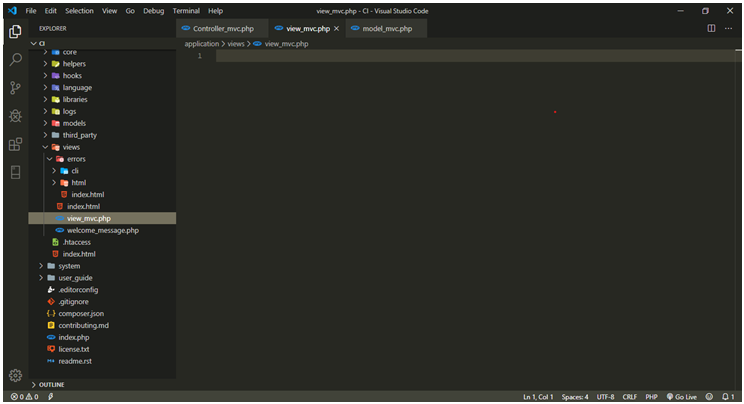
\includegraphics[width=0.95\textwidth]{figures/MVC/6.png}}
	\caption{Membuat File view\_mvc}
	\label{mvc6}
\end{figure}
%ada gambar

Jika tempilannya telah sama atau mirip seperti pada gambar \ref{mvc6} maka masukan code berikut pada file view\_mvc.php. walaupun ekstensi pada file tesebut merupakan php tapi isi code didalammnya merupakan tag HTML dikarenakan di gunakan untuk tampilan sehingga bisa lebih menarik.
\begin{lstlisting}[language=HTML]
<html>
<head>
    <title>
        contoh pemerograman mvc
    </title>
</head>
<body>
    <h3>
        <?php echo $data; ?>
    </h3>
</body>

</html>
\end{lstlisting}
\pagebreak
\textbf{Penjelasan \textit{Source Code}}.\par

Pada source code tersebut menggunakan tag html diakarenakan digunakan untuk menampilkan data yang telah di tampilkan controller. adapun penejelasan file view tersebut sebagai berikut:
\begin{enumerate}
\item file view dibuat dengan ekstensi php bukan html, dikarenakan codeigniter menggunakan base Php sehingga untuk view menggunakan ekstensi php hal ini bertujuan agar file view tersebut dapat dieksekusi atau di jalankan oleh controller.
\item pada baris ke satu dan 13 merupakan tag html
\item pada baris ke dua dan ke 6 merupakan tag head.
\item pada baris ke tiga dan lima merupakan tag title.
\item pada baris ke tujuh dan ke 11 merupakan tag body html 
\item kemudian pada body terdapat tag header tiga dan pada baris ke 4 merupakan variabel data yang merupakan parameter dari controller yang di kirim menggunakan array assosiatif. 
\end{enumerate}

Kemudian untuk menjalankan hasil dari codingan controller model dan view tersebut nyalakan terlebih dahulu xampp yaitu dengan menyalakan xampp control panel dan memilih start pada apache dan mysql, setelah itu buka web browser kemudian isikan alamat tersebut http://localhost/CI/index.php/Controller\_mvc maka hasilnya seperti pada gambar \ref{mvc7} berikut.

\begin{figure}[h]
	\centerline{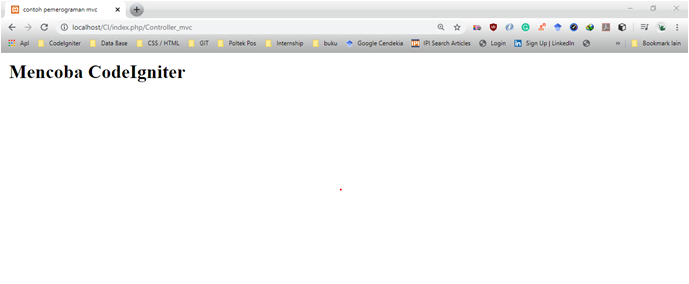
\includegraphics[width=0.95\textwidth]{figures/MVC/7.png}}
	\caption{view contoh mvc sederhana}
	\label{mvc7}
\end{figure}
%ada gambar

\pagebreak
	pada file view tersebut di dapat dikombinasikan  dengan bahasa pemrograman lain seperti css dan javascript,hal ini bisa dilakukan dengan cara menuliskan langsung source code css atau java script tersebut pada file tersebut atau bisa di lakukan dengan cara menimpan file css dan java script pada folder lain kemudian nanti pada tag html di panggil pada bagian header atau footer.
berikut ini merupakan source code untuk view yang di padukan dengan css, pada source code tersebut source code css di tuliskan pada file pada view.
\begin{lstlisting}[language=PHP]
<?php
defined('BASEPATH') or exit('No direct script access allowed');
?>
<!DOCTYPE html>
<html lang="en">

<head>
    <meta charset="utf-8">
    <title> contoh pemerograman mvc </title>

    <style type="text/css">
        ::selection {
            background-color: #E13300;
            color: white;
        }

        ::-moz-selection {
            background-color: #E13300;
            color: white;
        }

        body {
            background-color: #fff;
            margin: 40px;
            font: 13px/20px normal Helvetica, Arial, sans-serif;
            color: #4F5155;
        }

        a {
            color: #003399;
            background-color: transparent;
            font-weight: normal;
        }

        h1 {
            color: #444;
            background-color: transparent;
            border-bottom: 1px solid #D0D0D0;
            font-size: 19px;
            font-weight: normal;
            margin: 0 0 14px 0;
            padding: 14px 15px 10px 15px;
        }

        code {
            font-family: Consolas, Monaco, Courier New, Courier, monospace;
            font-size: 12px;
            background-color: #f9f9f9;
            border: 1px solid #D0D0D0;
            color: #002166;
            display: block;
            margin: 14px 0 14px 0;
            padding: 12px 10px 12px 10px;
        }

        #body {
            margin: 0 15px 0 15px;
        }

        p.footer {
            text-align: right;
            font-size: 11px;
            border-top: 1px solid #D0D0D0;
            line-height: 32px;
            padding: 0 10px 0 10px;
            margin: 20px 0 0 0;
        }

        #container {
            margin: 10px;
            border: 1px solid #D0D0D0;
            box-shadow: 0 0 8px #D0D0D0;
        }
    </style>
</head>

<body>

    <div id="container">
        <h1>Belajar Codeigniter MVC</h1>
        <div id="body">
            <p><?php echo $data ?></p>
        </div>
    </div>

</body>

</html>

\end{lstlisting} 
\pagebreak
\textbf{Penjelasan \textit{Source Code}}.\par
pada source code tersebut di gunakan untuk view pada dasarnya seperti php view seperti biasa, kemudian untuk menyisipkan source code atau link untuk memanggil css di tuliskan pada bagian header, atau pada source code tersebut pada baris ke tujuh samapai baris ke 76, lalu untuk source code tersebut merupakan css bawaan dari codeigniter.

Untuk hasinya seperti pada gambar \ref{mvc7} seperti berikut:

\begin{figure}[h]
	\centerline{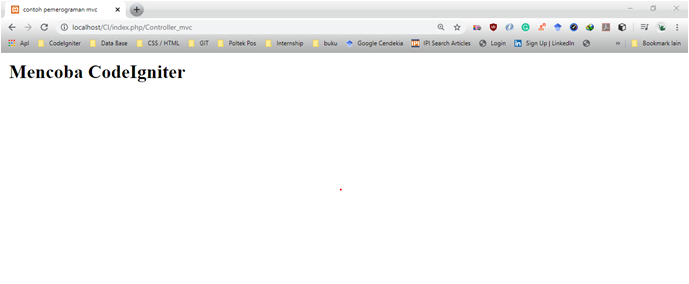
\includegraphics[width=0.95\textwidth]{figures/MVC/7.png}}
	\caption{view contoh mvc sederhana}
	\label{mvc7}
\end{figure}
 
%ada gambar


\section{ Penjelasan Mengirim data MVC}

Pada konsep mvc dikarenakan menggunakan class sehingga konsep turunan dari kelas pasti digunakan atau secara intinya konsep OOP sengat digunakan. Untuk itu berikut penjelasan cara mengirimkan data menggunakan konsep MVC pada codeigniter 
	Pada code model di contoh implementasi MVC terdapat code berikut:\par

\begin{lstlisting}[language=PHP]
public $str = ‘Mencoba CodeIgniter’ 
\end{lstlisting}
Source code tersebut merupakan objek sebagai variabel str dengan isi data string (Mencoba CodeIgniter) yang mana objek tersebut berstatus public yang berarti dapat di gunakan oleh class lain, sehingga jika data tersebut akan di ambil atau di gunakan pada controller harus mendekralasikan terlebih dahulu class dari model tersebut, contohnya yaitu seperti pada file Controller\_mvc terdapat source code seperti berikut.
\begin{lstlisting}[language=PHP]
$this->load->model(‘model_mvc’);
\end{lstlisting} 
Code tersebut berarti memanggil atau memuat model dari folder model dengan nama class dan file ‘model\_mvc’ code tersebut dapat di sisipkan pada setiap fungsi pada class yang berada pada controller, atau jika model tersebut di gunakan oleh banyak fungsi atau dominasi fungsi dapat menuliskannya pada pungsi konstruktor, kemudian untuk contoh menyisipkan code untuk memuat model seperti code tersebut:
\begin{lstlisting}[language=PHP]
    public function get_data()
    {
        $this->load->model('model_mvc');
        // code yang berkaitan dengan model
    }

\end{lstlisting} 
Yang di maksud contruktor yaitu fungsi yang di gunakan untuk meload atau memuat model, library dari codeigniter kemudian model atau library tersebut dapat di gunakan pada fungsi-fungsi yang terdapat pada class tersebut untuk contoh penulisan construktor, yaitu seperti pada source code berikut:
\begin{lstlisting}[language=PHP]
function __construct()
	{
		parent::__construct();
		$this->load->model('model_mvc');
	}

\end{lstlisting}  
Setelah meload atau memanggil model maka setiap fungsi dan objek yang berstatus public dapat di gunakan pada controller, pada contoh implementasi MVC tersebut yaitu menggunakan objek str untuk menggunakan data di dalammnya. Untuk dapat menggunakan atau memanggil data pada objek dapat dilakukan dengan cara seperti pada code berikut:
\begin{lstlisting}[language=PHP]
$data_model = $this->model_mvc;
$string = $data_model->str;

\end{lstlisting}

Pada variabel \$data\_model yang memuat model\_mvc kemudian untuk mengambil fungsi yang berada pada model dapat menggunakan vfariabel baru pada contoh terbut yaitu \$string dengan isi variabel \$data\_model kemudian merujuk pada str yang merupakan objek yang terdapat pada model. Selain menggunakan code tersebut dapat dilakukan seperti code tersebut sehingga menjadi lebih sederhana.

\begin{lstlisting}[language=PHP]
$string = $this->model_mvc->str
\end{lstlisting}
source code tersebut intinya sama yaitu mengambil data pada objek str yang terdapat pada file model\_mvc. Kemudian untuk mengirimkan data tersebut pada view harus menggunakan array asosiatif atau data harus berupa objek pada code implementasi MVC menggunakan code berikut 

\begin{lstlisting}[language=PHP]
$data['data'] = $string;
\end{lstlisting}

Variabel \$string merupakan data yang di kirim ke view yang berisikan data objek str dari model, code untuk mengirim data juga dapat di tuliskan seperti berikut: 

\begin{lstlisting}[language=PHP]
$data = array('data' => $string);
\end{lstlisting}

Atau bisa juga sebagai berikut

\begin{lstlisting}[language=PHP]
$data = ['data' => $string]
\end{lstlisting}

Code tersebut dapat diimplementasikan pada php 5.4 atau versi di atasnya.
Untuk mengirimkan data tersebut pada view dilakukan pada saat memuat view yaitu dengan menjadikan variabel \$data menjadi parameter seperti pada code berikut

\begin{lstlisting}[language=PHP]
$this->load->view('view_mvc', $data);
\end{lstlisting}

Berdasarkan code tersebut maka code tersebut juga dapat di ruliskan seperti berikut:

\begin{lstlisting}[language=PHP]
$this->load->view(‘view_mvc’, array('data' => $string));
\end{lstlisting}
atau
\begin{lstlisting}[language=PHP]
$this->load->view(‘view_mvc’, ['data' => $string]);
\end{lstlisting}

data merupakan kunci dari array asosiatif yang digunakan untuk memanggil data pada view yaitu dengan cara merubanya menjadi variabel yaitu dengan menambahkan tanda seperti berikut(\$) sebagai contoh pada view dapat di panggil seperti berikut  

\begin{lstlisting}[language=PHP]
<?php echo $data ?>
\end{lstlisting}
Atau 
\begin{lstlisting}[language=PHP]
<?= $data ?>
\end{lstlisting}
\begin{lstlisting}[language=PHP]

\end{lstlisting}
%\ref{lst:flcs}:
%\lstinputlisting[caption=File flasklivechart.py,label={lst:flcs}]{src/mia.py}











\chapter{Metode Entropy}
Pada Bab Ini akan membahas mengenai metode entropy,
Kelebihan dan kekurangan metode entropy 
Penjelasan dari rumus metode entropy
Penjelasan mengenai cara penggunaan metode entropy
Jenis data yang bisa diolah menggunakan metode entropy kemudian penggunaan entropy pada sistem
\pagebreak

\section{Metode Entropy}

Metode entropy merupakan metode yang di gunakan untuk menentukan tingkat kepentingan dari keriteria atau pembobotan untuk keriteria  selain itu metode ini juga dapat di gunakan untuk menentukan tingkat kepentingan awal atau bobot awal dari keriteria \cite{harahap2017penerapan}, \cite{chai2018new}. Sehingga walaupun di perhitungan awal bobot dari nilai entropy kecil pada suatu keriteria milaslkan dikarenakan variasi data yang kecil pada keriteria tersebut, namun jika keriteria tersebut di anggap penting oleh pengambil keputusan maka dia dapat memberikan bobot yang tinggi pada criteria tersebut, kedua bobot tersebut kemudian dapat di kalkulasikan sehingga mendapatkan nilai entropy akhir Lalu metode ini dapat menyelidiki keserasian dalam diskriminasi diantara sekumpulan data\cite{malekian2016application} . Nilai-nilai alternatif pada kriteria tertentun digambarkan dalam secision matrix (DM). dengan menggunakan metode entropy dengan variasi nilai tertinggi akan mendapatkan nilai tertinggi \cite{meiriza2019implementasi}.

Pada buku ini salah satu rumus entropy yang akan di bahas yaitu metode entropy shannons atau shannons entropy, yang memiliki persamaan atau rumus seperti pada gambar \ref{r1} berikut ini:

\begin{figure}[h]
	\centerline{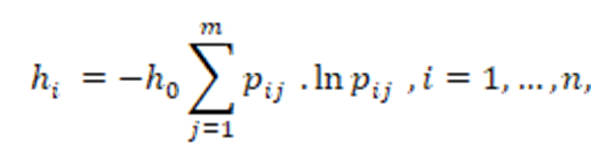
\includegraphics[width=0.6\textwidth]{figures/rumus/1.png}}
	\caption{Rumus Shanon's Entropy}
	\label{r1}
\end{figure}


Rumusan tersebut ditemukan Pada tahun 1948 Claude E. Shannon yang memperkenalkan entropy informasi sehingga sekarang sering di sebut dengan Entropy shannon, Selain digunakan untuk membobotkan setiap keriteria dari alternatif Metode ini juga dapat di gunakan untuk mengevaluasi bobot pada dasar subjektif dan objektif bobot \cite{wu2011determination}.

Maka dari itu berikut ini merupakan ada beberapa ketentuan data yang bisa di terapkan pada metode entropy ini, berikut merupakan ke tentuan ketentuannya:
\begin{enumerate}

\item Data dapat berupa data kualitatif 
\item Data juga dapat berupa data kuantitatif
\item Data-data tersebut harus dapat terukur 
\item Satuan untuk setiap keriteria boleh berbeda
\end{enumerate}
\pagebreak

\subsection{Kelebihan dan Kekurangan Entropy}

Setiap metode pasti ada kekurangan dan kelebihan maka dari itu berikut merupakan beberapa kekurangan dan kelebihan dari metode entropy:

Kelebihan dari metode ini diantaranya:\par
\begin{itemize}
\item Dapat membobotkan data baik itu data kualitatif atau data kuantitatif dengan catatan data tersebut dapt terukur atau memiliki nilai

\item Memberikan bobot awal untuk pengambilan keputusan
\end{itemize}
Kekurangan dari metode diantaranya:\par
\begin{itemize}
\item Hasil dari pembobotan bisa sangat kecil maupun sangat besar tergantung pada data nominal data yang di gunakan atau fariasi data yang kecil maupun besar.
\end{itemize}
\subsection{Tahapan Penggunaan Metode Entropy}
	Setiap metode pasti ada langkah-langkah atau tahapan untuk melakukan perhitungan dengan metode tersebut, begitupula dengan metode entropy terdapat tahapan-tahapan untuk menggunakan metode tersebut, maka dari itu berikut merupakan thapan-tahapan untuk menggunkan metode entropy:

\begin{enumerate}
\item Normalisasi terlebih dahulu data setiap keriteria, menggunakan persamaan atau sesuai dengan rumus pada gambar \ref{r2} berikut:

\begin{figure}[h]
	\centerline{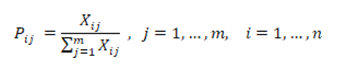
\includegraphics[width=0.6\textwidth]{figures/rumus/2.png}}
	\caption{Rumus Normalisasi Data}
	\label{r2}
\end{figure}

adapun arti dari rumus pada gambar tersebut seperti berikut:
\begin{itemize}
\begin{figure}[h]
	\centerline{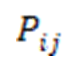
\includegraphics[width=0.1\textwidth]{figures/rumus/2-1.png}}
	\caption{Simbol Data delah dinormalisasi}
	\label{r3}
\end{figure}
\item pada gambar \ref{r3} merupakan simbol rumus dari data yang telah di normalisasi.
\pagebreak
\begin{figure}[h]
	\centerline{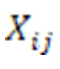
\includegraphics[width=0.1\textwidth]{figures/rumus/2-2.png}}
	\caption{Simbol Nilai Pada satu kolom}
	\label{r4}
\end{figure}
\item Pada gambar \ref{r4} merupakan simbol dari nilai yang terdapat pada satu kolom
\begin{figure}[h]
	\centerline{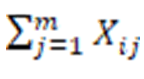
\includegraphics[width=0.1\textwidth]{figures/rumus/2-3.png}}
	\caption{Nilai total dari satu baris}
	\label{r5}
\end{figure}
\item  Pada gambar \ref{r5} merupakan simbol dari nilai total data yang berada pada satu baris yang sama.
\begin{figure}[h]
	\centerline{\includegraphics[width=0.1\textwidth]{figures/rumus/2-4.png}}
	\caption{Simbol Jumlah Baris Alternatif}
	\label{r6}
\end{figure}
\item pada gambar \ref{r6} merupaka simbol dari jumlah alternatif
\end{itemize}
agar lebih jelas dapat di lihat pada ilustrasi pada tabel 2.1 berikut:

\begin{table}[h]
\caption{Ilustrasi data yang dinormalisasi}
\centering
\begin{tabular}{|c|c|c|c|c|}
\hline
Alternatif & Kriteria 1 & Kriteria 2 & Kriteria 3 \\
\hline
1   & Xij & Xij& Xij\\
\hline
2   & Xij & Xij& Xij\\
\hline
3   & Xij & Xij& Xij\\
\hline
4   & Xij & Xij& Xij\\
\hline
5   & Xij & Xij& Xij\\
\hline
\end{tabular}
\label{as}
\end{table}

Dimana nilai total dari kriteria 1 yaitu Xij+Xij+Xij+Xij+Xij \par

sehingga contoh untuk mencari nilai pada alternatif 1 dan keriteria 1 seperti berikut:\par

Xij pada kolom ke satu baris ke satu dibagi dengan nilai total keriteria ke satu

\pagebreak

\item Setelah menormalisasi data tersebut lakukan perhitungan entropy menggunakan perasamaan pada gambar \ref{rr1}:

\begin{figure}[h]
	\centerline{\includegraphics[width=0.6\textwidth]{figures/rumus/1.png}}
	\caption{Rumus Shanon's Entropy}
	\label{rr1}
\end{figure}

Kemudian untuk arti dari rumus tersebut sebagai berikut:
\begin{itemize}
\begin{figure}[h]
	\centerline{\includegraphics[width=0.05\textwidth]{figures/rumus/3.png}}
	\caption{Simbol Nilai Entropy awal}
	\label{rr2}
\end{figure}
\item pada gambar \ref{rr2} tersebut merupakan tanda atau sintaks untuk Nilai Entropy Awal

\begin{figure}[h]
	\centerline{\includegraphics[width=0.1\textwidth]{figures/rumus/3-1.png}}
	\caption{Simbol Nilai Koefisiaen}
	\label{rr3}
\end{figure}

\item pada gambar \ref{rr3} tersebut merupakan tanda atau sintaks dari nilai koefisien, untuk mendapatkan nilai koefisien dapat dilakukan dengan menggunakan rumus pada gambar \ref{rr4}

\begin{figure}[h]
	\centerline{\includegraphics[width=0.12\textwidth]{figures/rumus/3-2.png}}
	\caption{Rumus Nilai Koefisien}
	\label{rr4}
\end{figure}

\item adapun penjelasan untuk rumus koefisien seperti berikut:

\begin{figure}[h]
	\centerline{\includegraphics[width=0.05\textwidth]{figures/rumus/3-3.png}}
	\caption{Simbol Nilai Logaritma}
	\label{rr5}
\end{figure}

pada gambar \ref{rr5} yaitu niali logaritma dari jumlah baris atau total alternatif
\pagebreak
\begin{figure}[h]
	\centerline{\includegraphics[width=0.05\textwidth]{figures/rumus/2-4.png}}
	\caption{Simbol Jumlah Alternatif}
	\label{rr6}
\end{figure}

pada gambar \ref{rr6} yaitu jumlah alternatif yang ada pada data.

\begin{figure}[h]
	\centerline{\includegraphics[width=0.4\textwidth]{figures/rumus/3-4.png}}
	\caption{Nila Total hasil kali data normalisasi}
	\label{rr7}
\end{figure}

pada gambar \ref{rr7} merupakan nilai total data normalisasi yang telah dikalikan dengan nilai normalisasi yang sebelumnya di kalikan dengan nilai normalisasi.\par
\end{itemize}

kemudian untuk tahapan implementasi dari rumus tersebut sebagai berikut:

\begin{itemize}
\item pertama cari nilai cari nilai dari koefisien dengan cara mempraktikan rumus koefisien, pada rumus tersebut terdapat pangkat -1 yang berarti 1 dibagi, sehingga dalam mengimplementasikan rumus koefisien yaitu dengan cara 1 di bagi dengan nilai log dari total baris kemudian nilainya ubah menjadi minus, hal ini di karenakan sudah ketentuan dari rumusan entropy.

\item kedua cari nilai perkalian data yang telah di normalisasi dengan data normalisasi yang sudah di kalikan dengan nilai log, agar lebih jelas contoh penempatannya seperti pada tabel 2.2 berikut ini:

\begin{table}[h]
\caption{Ilustrasi Perkalian data yang telah di normalisasi}
\centering
\begin{tabular}{|c|c|c|c|c|}
\hline
Alternatif & Kriteria 1 & Kriteria 2 & Kriteria 3 \\
\hline
1   & Pij * ln Pij & Pij * ln Pij & Pij * ln Pij \\
\hline
2   & Pij * ln Pij  & Pij * ln Pij & Pij * ln Pij \\
\hline
3   & Pij * ln Pij  & Pij * ln Pij & Pij * ln Pij \\
\hline
4   & Pij * ln Pij  & Pij * ln Pij & Pij * ln Pij \\
\hline
5   & Pij * ln Pij  & Pij * ln Pij & Pij * ln Pij \\
\hline

\end{tabular}
\label{table2}
\end{table}

\item setelah itu cari nilai total dari setiap baris keriteria dengan cara menambahkan data yang ada pada setiap baris yang terdapat pada setiap kriteria.

\item kemudian jika semua nilai total telah di dapatkan, kalikan nilai total tersebut dengan nilai koefisien yang sudah dalam keadaan negatif, untuk hasilnya pasti akan bernilai positif.
\end{itemize}

\pagebreak

\item Cari nilai bobot entropy akhir dengan menggunakan rumus pada gamabr \ref{rrr1} berikut:

\begin{figure}[h]
	\centerline{\includegraphics[width=0.6\textwidth]{figures/rumus/4.png}}
	\caption{Nila Total hasil kali data normalisasi}
	\label{rrr1}
\end{figure}
kemudian untuk penjelasan rumus pada gambar \ref{rrr1} tersebut sebagai berikut:

\begin{itemize}
\begin{figure}[h]
	\centerline{\includegraphics[width=0.05\textwidth]{figures/rumus/4-1.png}}
	\caption{Simbol Bobot Entropy}
	\label{rrr2}
\end{figure}
\item Pada gambar \ref{rrr2} merupakan gambar dari simbol bobot entropy
\begin{figure}[h]
	\centerline{\includegraphics[width=0.05\textwidth]{figures/rumus/4-2.png}}
	\caption{Simbol Keriteria Ke sekian}
	\label{rrr3}
\end{figure}
\item Pada gambar \ref{rrr3} merupakan gambar dari simbol keriteria ke sekian
\begin{figure}[h]
	\centerline{\includegraphics[width=0.05\textwidth]{figures/rumus/4-3.png}}
	\caption{Nilai Hasil Kurang antara satu dengan nilai entropy pertama}
	\label{rrr4}
\end{figure}
\item Pada gambar \ref{rrr4} merupakan gambar dari simbol hasil kurang antara satu dengan nilai entropy yang pertama
\begin{figure}[h]
	\centerline{\includegraphics[width=0.13\textwidth]{figures/rumus/4-4.png}}
	\caption{Nila Total dari hasi kurang}
	\label{rrr5}
\end{figure}
\item Pada gambar \ref{rrr5} merupaka simbol dari nilai total hasil pengurangan antara 1 (satu) dengan bobot awal
\end{itemize}

Untuk tahapan mencari nilai total dapat di lakukan dengan cara seperti berikut ini:

\begin{itemize}
\item setelah nilai total dari hasil perkalian data yang telah di normalisasi dan nilai koefisien ditemukan, data tersebut dijadikan sebagai pengurang dari niali 1 (satu), nilai satu tersebut merupakan nilai ketentuan dari rumus bobot entropy total.

\item kemudian jika semua nilai telah di temukan dari setiap keriteria maka cari nilai total dari hasil pengurangan yang di lakukan pada setiap keriteria, sehingga di dapatkan nilai total dari hasil pengurangan tersebut.

\item jika nilai total sudah di temukan maka nilai total tersebut menjadi pembagi untuk setiap data yang telah di kurangi.
\end{itemize}

\textbf{Catatan :}\par
\textit{Pada saat mencari nilai bobot akhir dilakukan pembagian dari nilai pengurangan dari setiap criteria dengan nilai total dari semua pengurangan dari semua keriteria, atau untuk lebih jelasnya dapat di lihat pada contoh perhitungan entropy pada BAB 3}
\end{enumerate}

\subsection{Contoh Kasus Dalam Penerapan Metode Entropy}

Dalam penerapannya metode ini dapat di terapkan pada beberapa kasus pengambilan keputusan, contohnya seperti pada kasus pengambilan keputusan untuk memilih siswa terbaik \cite{majdi2017penerapan}, kemudian dalam pembobotan untuk memilih supplier bahan baku \cite{saputra2016usulan}, selain itu metode ini juga dapat di terapkan pada kasus untuk pemilihan perawatan saluran air \cite{brankovic2018comparative} selain itu metode ini juga dapat di gunakan untuk mengevaluasi sesuatau contohnya seperti mengevaluasi hasil operasi perusahaan jaringan listrik \cite{wu2018comprehensive}, kemudian untuk contoh lainnya metode entropy juga dapat digunakan untuk mencari bobot untuk perangkingan atau urutan \cite{harahap2017penerapan}.

\section{Implementasi Metode Entropy Pada Sistem}

 Pada contoh sistem yang di buat pada aplikasi ini metode entropy di terapkan pada bagian menu Proses entropy, namun sebelum masuk ke menu tersebut terlebih dahulu untuk setiap user pengguna sistem melengkapi terlebih dahulu data yang terdapat pada menu data alternatif, hal ini disebabkan karena data yang dilakukan pembobotan menggunakan metode entropy ini menggunakan data yang terdapat pada tabel alternatif. Jika data yang terdapat pada menu data alternetif telah ada dan lebih dari 2 (dua) data, maka proses entropy dapat di lakukan. kemudian agar lebih jelas untuk tahapan-tahapan proses entropy pada sistem seperti berikut ini:
\pagebreak
\begin{enumerate}
\item klik menu Proses entropy seperti pada gambar \ref{ro1} dan gambar \ref{ro2} berikut 

\begin{figure}[h]
	\centerline{\includegraphics[width=0.9\textwidth]{figures/pje/1.png}}
	\caption{Menu entropy pada halaman utama admin}
	\label{ro1}
\end{figure}

\begin{figure}[h]
	\centerline{\includegraphics[width=0.9\textwidth]{figures/pje/2.png}}
	\caption{Menu Entropy pada halaman utama selain admin}
	\label{ro2}
\end{figure}
\pagebreak
\item kemudian jika telah masuk ke menu proses entropy masukan id user pada form seperti pada gambar \ref{ro3} berikut ini.

\begin{figure}[h]
	\centerline{\includegraphics[width=0.90\textwidth]{figures/pje/3.png}}
	\caption{Form insert user id}
	\label{ro3}
\end{figure}

\item setelah itu klik tombol kirim pada form tersebut kemudian hasil dari perhitungan entropy akan muncul seperti pada gambar \ref{ro4} berikut 

\begin{figure}[h]
	\centerline{\includegraphics[width=0.90\textwidth]{figures/pje/4.png}}
	\caption{Hasil Perhitungan Entropy}
	\label{ro4}
\end{figure}
\pagebreak
\item jika data bobot hasil entropy dirasa di butuhkan atau akan segera di gunakan bisa menekan tombol simpan data entropy seperti pada gambar \ref{ro5} berikut 

\begin{figure}[h]
	\centerline{\includegraphics[width=0.80\textwidth]{figures/pje/5.png}}
	\caption{Menyimpan Data Entropy}
	\label{ro5}
\end{figure}

\item maka hasil data yang telah disimpan akan masuk ke basis data sistem yang hasilnya terdapat pada menu data bobot seperti pada gambar \ref{ro6} berikut

\begin{figure}[h]
	\centerline{\includegraphics[width=0.80\textwidth]{figures/pje/6.png}}
	\caption{Data Bobot yang telah di simpan}
	\label{ro6}
\end{figure}
\end{enumerate}

\textbf{Catatan :}\par
\textit{Pada tahapan tersebut sebenarnya ada perbedaan untuk user admin dan user pengguna sistem biasa atau yang levelnya di bawah admin, jika user yang login ke sistem bukan user admin maka tidak perlu melakukan input id user hanya perlu menekan menu proses entropy maka akan muncul hasil seperti pada tahapan ke 3, kemudian untuk proses menyimpan data entropy sama seperti pada user admin. Selain itu Proses ini hanya dapat dilakukan jika data lebih dari dua atau minimal dua baris data.}



\chapter{Implementasi Perhitungan Entropy}
Pada bab ini akan membahas mengenai implementasi metode entropy, implementasi di sini yaitu ke cara penggunaan metode entropy, setelah itu dilanjutkan dengan contoh-contoh perhitungan dari metode entropy selain itu pada bab ini terdapat tiga contoh perhitungan metode entropy dengan berbagai keadaan atau studi kasus yang berbeda.
\pagebreak

\section{Persiapan Data}

	Sebelum masuk ke dalam perhitungan data, data yang akan diolah harus dipersiapkan misalkan jumlamnya data yang akan terlibat untuk melakukan proses entropy, selanjutnya jenis keriteria yang digunakan kemudian tujuan pembobotan dengan entropy berikut merupakan tiga tabel data yang akan di olah menggunakan metode entropy:

\begin{table}[h]
\caption{Data Handphone dan spesifikasinya 1}
\centering
\begin{tabular}{|c|c|c|c|c|}
\hline
Alternatif & Harga & Kamera & Batrai&Memori\\
\hline
Handphone 1 &1000 & 10 MP & 2000 mAh &  16 GB\\
\hline
Handphone 2 &2000 & 10 MP & 3500 mAh &  32 GB\\
\hline
Handphone 3 &1500 & 13 MP & 2000 mAh &  32 GB\\
\hline

\end{tabular}
\label{T3}
\end{table}

Pada tabel \ref{T3} tersebut terdapat data handphone dan spesifikasinya yang akan dihitung menggunakan metode entropy untuk mengetahui bobot dari setiap kriteria pada data tersebut, untuk proses perhitungannya dapat dilihat pada proses perhitungan entropy ke 1

\begin{table}[h]
\caption{Data Handphone dan spesifikasinya 2}
\centering
\begin{tabular}{|c|c|c|c|c|c|}
\hline
Alternatif & Harga & Kamera depan & Kamera Belakang&RAM& Memori\\
\hline
Handphone 1 &300& 5 MP & 24 MP &  2 GB&64 GB\\
\hline
Handphone 2 &250 & 5 MP & 13 MP &  2 GB&32 GB\\
\hline
Handphone 3 &330 & 13 MP & 24 MP &  3 GB&64 GB\\
\hline
Handphone 4 &330 & 5 MP & 8 MP &  2 GB&32 GB\\
\hline
Handphone 5 &330 & 2 MP & 5 MP &  2 GB&16 GB\\
\hline

\end{tabular}
\label{T4}
\end{table}

kemudian pada tabel \ref{T4} merupakan tabel yang digunakan untuk perhitugan entropy, data tersebut hampirsama seperti pada data di tabel \ref{T3} yang merupakan data handphone, hanyasaja pada data ini untuk keriteria bertambah kemudian jumlah dari alternatif yang terlibat dalam perhitungan juga bertambah, kemudian untuk peroses perhitunggannya terdapat pada proses perhitungan entropy ke 2.\par
\pagebreak
terakhir terdapat data nilai siswa yang terdapat pada tabel \ref{T5} berikut:

\begin{table}[h]
\caption{Data Nilai Siswa}
\centering
\begin{tabular}{|c|c|c|c|c|}
\hline
Alternatif & MTK & IPS & IPA&BI\\
\hline
Siswa 1 &92 & 70 & 88 &  65\\
\hline
Siswa 2 &70 & 80 & 58 &  76\\
\hline
Siswa 3 &83 & 60 & 75 &  80\\
\hline
Siswa 4 &60 & 87 & 67 &  60\\
\hline
Siswa 5 &55 & 89 & 76 &  87\\
\hline

\end{tabular}
\label{T5}
\end{table}

pada tabel \ref{T5} merupakan data nilai dari lima siswa, dimana dari keriteria nilai dari setiap alternatifnya akan diambil bobot dari setiap kriteria. untuk proses perhitungannya terdapat pada subbab proses perhitungan entropy ke 3

\section{Proses Perhitungan Entropy Ke 1}

	Dalam mencari entropy untuk setiap keriteria terdapat beberapa peroses, proses tersebut diantaranya yaitu:

menormalisasi data pada tabel \ref{T3} sehingga hasilnya seperti tabel \ref{table4} berikut ini:
\begin{table}[h]
\caption{Data Normalisasi}
\centering
\begin{tabular}{|c|c|c|c|c|}
\hline
Alternatif & Harga & Kamera & Batrai&Memori\\
\hline
Handphone 1 &1000 & 10 & 2000 &  16\\
\hline
Handphone 2 &2000 & 10 & 3500 &  32\\
\hline
Handphone 3 &1500 & 13 & 2000 &  32\\
\hline

\end{tabular}
\label{table4}
\end{table}

setelah melakukan normalisasi data cari nilai total dari setiap kriteria, dengan cara menambahkan setiap data pada baris keriteria jika telah selesai maka akan di dapatkan nilai total dari setiap keriteria seperti pada tabel \ref{table5} tersebut

\begin{table}[h]
\caption{Nilai Total Normalisasi}
\centering
\begin{tabular}{|c|c|c|c|}
\hline
 Harga & Kamera & Batrai&Memori\\
\hline
4500 & 33 & 7500 &  80\\
\hline
\end{tabular}
\label{table5}
\end{table}

jika nilai total untuk setiap keriteria telah di dapatkan maka dilanjutkan dengan menormalisasi data tersebut yaitu dengan menjadikan nilai total tersebut sebagai pembagi untuk setiap data yang terdapat pada baris keriteria, untuk setiap data nilai total hanya bisa menjadi pembagi dari kriteria yang bersangkutan contoh seperti mendapatkan nilai total dari keriteria 1 maka nilai total tersebut hanya bisa membagi data yang terdapat pada baris keriteria 1 saja.
\pagebreak
untuk lebih jelasnya seperti pada tabel \ref{table6} tersebut.

\begin{table}[h]
\caption{Data pembagi}
\centering
\begin{tabular}{|c|c|c|c|c|}
\hline
Alternatif & Harga & Kamera & Batrai&Memori\\
\hline
Handphone 1 &1000/4500 & 10/33 & 2000/7500 &  16/80\\
\hline
Handphone 2 &2000/4500 & 10/33 & 3500/7500 &  32/80\\
\hline
Handphone 3 &1500/4500 & 13/33 & 200/75000 &  32/80\\
\hline

\end{tabular}
\label{table6}
\end{table}

kemudian jika semua data telah dibagi dengan nilai total maka akan mendapatkan hasil, pada tabel \ref{table7} merupakan hasil dari pembagian data yang di lakukan pada tabel \ref{table6}.

\begin{table}[h]
\caption{Data Normalisasi}
\centering
\begin{tabular}{|c|c|c|c|c|}
\hline
Alternatif & Harga & Kamera & Batrai&Memori\\
\hline
Handphone 1 &0.222 & 0.303 & 0.267 &  0.2\\
\hline
Handphone 2 &0.444 & 0.303 & 0.467 &  0.4\\
\hline
Handphone 3 &0.333 & 0.393 & 0.267 &  0.4\\
\hline

\end{tabular}
\label{table7}
\end{table}

jika telah mendapatkan nilai yang telah dinormalisasi maka di lanjutkan dengan mencari nilai koefisien dengan menggunakan rumus pada gambar \ref{rm1} tersebut, sebenarnya rumus tersebut sama saja seperti pada rumus koefisiensi yang telah dibahas pada bab 2 hanya saja rumus tersebut merupa kan bentuk lain atau cara penulisan lain dari rumus koefisien pada bab 2.

\begin{figure}[h]
	\centerline{\includegraphics[width=0.2\textwidth]{figures/rumus/5.png}}
	\caption{rumus koefisien}
	\label{rm1}
\end{figure}

diketahui alternatif pada data tersebut sebanyak 3 buah maka nilai koefisien dari rumus tersebut adalah 0,910239227\par
kemudian jika nilai koefisien telah di temukan maka selanjutnya lakukan perkalian nilai yang teelah di normalisasi dengan nilai yang telah dinormalisasi yang dikalikan terlebih dahulu dengan log (ln), untuk lebih jelasnya seperti pada tabel \ref{table8}.
\pagebreak
\begin{table}[h]
\caption{Perkalian nilai normalisasi}
\centering
\begin{tabular}{|c|c|c|c|c|}
\hline
Alternatif & Harga & Kamera & Batrai&Memori\\
\hline
Handphone 1 &(0.222) * ln (0.222) & (0.303) * ln (0.303) & (0.267) * ln (0.267) &  (0.2) * ln (0.2)\\
\hline
Handphone 2 &(0.444) * ln (0.444) & (0.303) * ln (0.303) & (0.467) * ln (0.467)  & (0.4) * ln (0.4)\\
\hline
Handphone 3 &(0.333) * ln (0.333) & (0.393) * ln (0.393) & (0.267) * ln (0.267) &  (0.4) * ln (0.4)\\
\hline

\end{tabular}
\label{table8}
\end{table}

jika telah melakukan perkalian tersebut maka akan mendapatkan hasil, maka dari itu berikut pada tabel \ref{table9} merupakan hasil dari perkalian data yang telah di normalisasi.
\begin{table}[h]
\caption{Data Hasil Kali Nilai Normalisasi}
\centering
\begin{tabular}{|c|c|c|c|c|}
\hline
Alternatif & Harga & Kamera & Batrai&Memori\\
\hline
Handphone 1 &-0,334127293 & -0,361788809 & -0,352575268 & -0,321887582\\
\hline
Handphone 2 &-0,36050 & -0,361788809 & -0,355585952 & -0,366516293\\
\hline
Handphone 3 &-0,366171059 & -0,367040647 & -0,352575268 & -0,366516293\\
\hline
\end{tabular}
\label{table9}
\end{table}

dari data pada tabel \ref{table9} tersebut cari lagi nilai total dari data tersebut, seperti biasa dengan menambahkan nilai dari setiap keriteria namun pada setiap baris ke bawah, bukan menjumlahkan setiap kolom (ke pinggir). 

\begin{table}[h]
\caption{Nilai total data hasil kali}
\centering
\begin{tabular}{|c|c|c|c|}
\hline
 Harga & Kamera & Batrai&Memori\\
\hline
-1,06079559 & -1,090618266 & -1,060736487 &  -1,054920168\\
\hline
\end{tabular}
\label{table10}
\end{table}

jika telah di cari nilai total dari setiap keriteria maka akan menghasilkan hasil seperti pada tabel \ref{table10} tersebut, dikarenakan tadi telah menemukan nilai koefisien dari data tersebut maka kalikan nilai koefisien tersebut dengan nilai total dari setiap keriteria seperti pada tabel \ref{table11} tersebut.

\begin{table}[h]
\caption{nilai total di kali nilai Koefisien}
\centering
\begin{tabular}{|c|c|c|c|}
\hline
 Harga & Kamera & Batrai&Memori\\
\hline
-0,910239227 & -0,910239227 & -0,910239227 &  -0,910239227\\
\hline
* & * & * &  *\\
\hline
-1,06079559 & -1,090618266 & -1,060736487 &   -1,054920168\\
\hline
\end{tabular}
\label{table11}
\end{table}
\pagebreak
kemudian untuk hasil dari perkalian pada tabel \ref{table11} tersebut dapat di lihat pada tabel\ref{table12} berikut ini.

\begin{table}[h]
\caption{Hasil Perkalian Nilai total dengan koefisien}
\centering
\begin{tabular}{|c|c|c|c|}
\hline
 Harga & Kamera & Batrai&Memori\\
\hline
0,965577757 & 0,992723527 &0,96552396 & 0,960229718\\
\hline
\end{tabular}
\label{table12}
\end{table}

jika telah menemukan hasil seperti pada tabel \ref{table12} tersebut maka nilai-nilai tersebut dijadikan pengurang dari nilai 1 (satu), dimana satu tersebut merupakan nilai atau ketentuan dari rumus entropy itu sendiri untuk prosesnya seperti pada tabel \ref {table13}.

\begin{table}[h]
\caption{satu di kurangi hasil perkalian nilai total dengan koefisien}
\centering
\begin{tabular}{|c|c|c|c|}
\hline
 Harga & Kamera & Batrai&Memori\\
\hline
1-0,965577757 &1-0,992723527 &1-0,96552396&1-0,960229718\\
\hline
\end{tabular}
\label{table13}
\end{table}

lalu jika data tersebut telah di kurangkan maka akan mendapatkan hasil seperti pada tabel \ref{table14}
\begin{table}[h]
\caption{Hasil pengurangan}
\centering
\begin{tabular}{|c|c|c|c|}
\hline
 Harga & Kamera & Batrai&Memori\\
\hline
0,034422&0,007276 &0,034476&0,03977\\
\hline
\end{tabular}
\label{table14}
\end{table}
kemudian jika telah mendapatkan hasil seperti pada tabel \ref{table14} lanjutkan dengan menambahkan semua hasil pengurangan tersebut, atau di cari nilai total dari hasil pengurangan tersebut. maka dari itu berikut merupakan hasil nilai total dari hasil pengurangan tersebut.\par

Niali total dari hasil pengurangan tersebut adalah 0,115945

kemudian jika nilai total telah ditemukan maka nilai total tersebut dijadikan pembagi untuk setiap data hasil pengurangan yang terdapat pada setiap keriteria untuk caranya seperti pada tabel \ref{table15} berikut ini 
\begin{table}[h]
\caption{Pembagian nilai total dengan hasil pengurangan}
\centering
\begin{tabular}{|c|c|c|c|}
\hline
 Harga & Kamera & Batrai&Memori\\
\hline
0,034422 /
0,115945
&0,007276
/ 0,115945
&0,034476
/ 0,115945
&0,03977
/ 0,115945
\\
\hline
\end{tabular}
\label{table15}
\end{table}
\pagebreak
dari hasil pembagian tersebut maka akan di hasilkan nilai untuk bobot kriteria atau sering disebut nilai entropy akhir dari setiap keriteria yang mana hasilnya dapat dilihat pada tabel \ref{table16} berikut ini. 

\begin{table}[h]
\caption{Bobot akhir setiap keriteria}
\centering
\begin{tabular}{|c|c|c|c|}
\hline
 Harga & Kamera & Batrai&Memori\\
\hline
0,296884138&0,06275795 &0,29734813&0,343009782\\
\hline
\end{tabular}
\label{table16}
\end{table}

untuk memeriksa apakah nilai bobot tersebut sudah benar maka tinggal tambahkan keseluruhan data bobot dari kriteria maka akan mendapatkan hasil nilai 1 (satu) yang berarti nilai 100\%.

\section{Proses Perhitungan Entropy Ke 2}

Dari Proses perhitungan entropy ke satu niali total dari bobot akan tetap satu walaupun keriteria di tambah menjadi 5 dan seterusnya, untuk membuktikannya brikut merupakan contoh perhitungan entropy ke 2 yang di gunakan untuk membobotkan criteria dari alternatif.\par
	Pada contoh data berikut merupakan contoh data penentuan bobot dari 5(lima) alternatif yaitu yang di misalkan sebagai handphone yang masing-masing memiliki lima keriteria diantaranya terdiri dari Harga (satuan Dolar), kamera depan (tolak ukur pixcel), kamera belakang (tolak ukur pixcel), RAM ( tolak ukur gigabyte (GB)) kapasitas batarai (torakukur mAh), dan Memory penyimpanan ( tolak ukur gigabyte (GB)). Untuk lebih jelasnya berikut merupakan contoh data untuk menentukan bobot criteria.

maka dari itu berikut merupakan data pada tabel \ref{TA1} yang digunakan sebagai bahan untuk perhitungan pada peroses entropy ke 2.


\begin{table}[h]
\caption{Data Handphone dan spesifikasinya 2}
\centering
\begin{tabular}{|c|c|c|c|c|c|}
\hline
\multirow{2}{*}{Alternatif} &\multirow{2}{*}{ Harga}& Kamera & Kamera&\multirow{2}{*}{RAM}& \multirow{2}{*}{Memori}\\
& & depan & belakang & &\\
\hline
Handphone 1 &300& 5 & 24 &  2&64\\
\hline
Handphone 2 &250 & 5 & 13 &  2&32\\
\hline
Handphone 3 &330 & 13 & 24 &  3 &64\\
\hline
Handphone 4 &330 & 5 & 8 &  2 GB&32\\
\hline
Handphone 5 &330 & 2 & 5 &  2 GB&16\\
\hline

\end{tabular}
\label{TA1}
\end{table}

\pagebreak

kemudian dari data pada tabel \ref{TA1} tersebut cari nilai total dari setiap keriteria, jika sudah menemukan nilai total setiap keriteria maka datanya akan seperti pada tabel \ref{TA2} berikut:

\begin{table}[h]
\caption{Nilai Total Setiap Alternatif}
\centering
\begin{tabular}{|c|c|c|c|c|}
\hline
 Harga & Kamera depan & Kamera Belakang&RAM& Memori\\
\hline
1280& 30 & 74 & 11 & 208\\
\hline
\end{tabular}
\label{TA2}
\end{table}

setelah nilai total untuk setiap keriteria di temukan atau didapatkan maka di lanjutkan dengan menormalisasi data dengan menjadikan nilai total dari setiap keriteria tersebut sebagai pembagi untuk setiap data atau nilai yang terdapat pada baris keriteria masing-masing, agar lebh jelas proses pembagian nilainnya seperti pada tabel \ref{TA3} berikut:

\begin{table}[h]
\caption{Normalisasi Data}
\centering
\begin{tabular}{|c|c|c|c|c|c|}
\hline
\multirow{2}{*}{Alternatif} &\multirow{2}{*}{ Harga}& Kamera & Kamera&\multirow{2}{*}{RAM}& \multirow{2}{*}{Memori}\\
& & depan & belakang & &\\
\hline
Handphone 1 &300/1280& 5/30 & 24/74 &  2/11&64/208\\
\hline
Handphone 2 &250/1280 & 5/30 & 13/74 &  2/11&32/208\\
\hline
Handphone 3 &330/1280 & 13/30 & 24/74 &  3/11 &64/208\\
\hline
Handphone 4 &330/1280 & 5/30 & 8/74 &  2/11&32/208\\
\hline
Handphone 5 &330/1280 & 2/30 & 5/74 &  2/11&16/208\\
\hline

\end{tabular}
\label{TA3}
\end{table}

	jika data telah di lakukan pembagian maka akan mendapatkan nilai hasi pembagian, pada tabel \ref{TA4} berikut merupakan hasil dari proses pembagian nilai olen nilai total dari setiap kriteria.

\begin{table}[h]
\caption{Hasil Normalisasi}
\centering
\begin{tabular}{|c|c|c|c|c|c|}
\hline
\multirow{2}{*}{Alternatif} &\multirow{2}{*}{ Harga}& Kamera & Kamera&\multirow{2}{*}{RAM}& \multirow{2}{*}{Memori}\\
& & depan & belakang & &\\
\hline
Handphone 1 &0,234375& 0,166667 & 0,324324 & 0,181818 & 0,307692\\
\hline
Handphone 2 & 0,195313 & 0,166667 & 0,175676 & 0,181818 & 0,153846\\
\hline
Handphone 3 & 0,257813 & 0,433333& 0,324324 & 0,272727 & 0,307692\\
\hline
Handphone 4 & 0,164063 & 0,166667& 0,108108 & 0,181818 & 0,153846\\
\hline
Handphone 5 & 0,148438 & 0,166667& 0,067568 & 0,181818 & 0,076923\\
\hline
\end{tabular}
\label{TA4}
\end{table}

Setelah data selesai di normalisasi dengan hasil data seperti pada tabel \ref{TA4} tersebut maka lanjutkan ke proses persamaan entropy, cari nilai koefisien untuk data tersebut menggunakan rumus koefisien pada gambar \ref{rmm1} berikut:

\begin{figure}[h]
	\centerline{\includegraphics[width=0.2\textwidth]{figures/rumus/5.png}}
	\caption{rumus koefisien}
	\label{rmm1}
\end{figure}

yang dimana pada data tersebut terdapat total jumlah alternatif sebanyak 5 , di karenakan pada data tersebut mempunyai lima alternatif maka nilai koefisien akan menjadi 0,621334935 \par

kemudian jika prosen mencari koefisien telah selesai maka selanjutnya cari nilai antara perkalian nilai yang telah di normalisasi dengan nilai normalisasi yang telah di kalikan dengan Ln (log).agar lebih jelas pada tabel \ref{TA5} berikut merupakan peroses perhitungan perkalian nilai yang telah di normalisasi.
\begin{table}[h]
\caption{Data Handphone dan spesifikasinya 2}
\centering
\begin{tabular}{|c|c|c|c|c|c|}
\hline
\multirow{2}{*}{Alternatif} &\multirow{2}{*}{ Harga}& Kamera & Kamera&\multirow{2}{*}{RAM}& \multirow{2}{*}{Memori}\\
& & depan & belakang & &\\
\hline
\multirow{3}{*}{Handphone 1} & (0,234375) & (0,166667)& (0,324324) &(0,181818) &(0,307692) \\
&* ln  &* ln  &* ln  &* ln  & * ln \\
&(0,234375) & (0,166667) &(0,324324) &(0,181818) &(0,307692)\\
\hline
\multirow{3}{*}{Handphone 2}&(0,195313)&(0,166667&(0,175676) &(0,181818) &(0,153846) \\
&* ln  &* ln  &* ln  &* ln  & * ln \\
&(0,195313)&(0,166667&(0,175676) &(0,181818) &(0,153846)\\
\hline
\multirow{3}{*}{Handphone 3}&(0,257813)&(0,433333) &(0,324324)&(0,272727)&(0,307692)\\
&* ln  &* ln  &* ln  &* ln  & * ln \\
&(0,257813)&(0,433333) &(0,324324)&(0,272727)&(0,307692)\\
\hline
\multirow{3}{*}{Handphone 4}&(0,164063)&(0,166667)&(0,181818)&(0,108108)&(0,153846)\\
&* ln  &* ln  &* ln  &* ln  & * ln \\
&(0,164063)&(0,166667)&(0,108108)&(0,181818)&(0,153846)\\
\hline
\multirow{3}{*}{Handphone 5}&(0,148438)&(0,066667)&(0,067568)&(0,181818)&(0,076923)\\
&* ln  &* ln  &* ln  &* ln  & * ln \\
&(0,148438)&(0,066667)&(0,067568)&(0,181818)&(0,076923)\\
\hline
\end{tabular}
\label{TA5}
\end{table}

kemudian jika perhitungan tersebut telah selesai maka hasilnya akan seperti pada tabel \ref{TA6} berikut ini, kemudian semua nilai yang ada pada tabel tersebut akan dalam keadaan negatif.
\pagebreak
\begin{table}[h]
\caption{Hasil Normalisasi}
\centering
\begin{tabular}{|c|c|c|c|c|c|}
\hline
\multirow{2}{*}{Alternatif} &\multirow{2}{*}{ Harga}& Kamera & Kamera&\multirow{2}{*}{RAM}& \multirow{2}{*}{Memori}\\
& & depan & belakang & &\\
\hline
Handphone 1 &-0,34004& -0,29863 &-0,36519 & -0,30995 & -0,362663\\
\hline
Handphone 2 &-0,31898 & -0,29863 & -0,30552 & -0,30995 & -0,28797\\
\hline
Handphone 3 &-0,34947 & -0,36237& -0,36519 & -0,35435 & -0,362663\\
\hline
Handphone 4 & -0,29654 & -0,29863& -0,2405 &-0,30995 & -0,28797\\
\hline
Handphone 5 &-0,28316 & -0,18054&-0,18207& -0,30995 & -0,197304\\
\hline
\end{tabular}
\label{TA6}
\end{table}

kemudian jika telah mendapatkan hasil seperti pada tabel \ref{TA6} tersebut dilanjutkan dengan mencari nilai total dari setiap keriteria dari tabel \ref{TA6} tersebut, dengan cara menambahkan setiap data keriteria dari data alternatif satu sampai data alternatif terakhir pada data tersebut.

\begin{table}[h]
\caption{Nilai Total Setiap Alternatif}
\centering
\begin{tabular}{|c|c|c|c|c|}
\hline
\multirow{2}{*}{ Harga}& Kamera & Kamera&\multirow{2}{*}{RAM}& \multirow{2}{*}{Memori}\\
& depan & belakang & &\\
\hline
-1,58819& -1,43879 & -1,45848 & -1,59417 & -1,498569\\
\hline

\end{tabular}
\label{TA7}
\end{table}

pada tabel \ref{TA7} merupakan hasil nilai total yang di dapatkan dari tabel \ref{TA6} dimana nilai total terdiri dari lima nilai total dari lima keriteria yaitu nilai tital harga, nilai tital kamera depan, belakang, nilai total RAM dan nilai total Memory.\par

kemudian setelah nilai total di dapatkan lanjutkan dengan mengalikan nilai total tersebut dengan nilai ln atau koefisien yang telah di cari terlebih dahulu, untuk caranya seperti pada tabel \ref{TA8} berikut ini.


\begin{table}[h]
\caption{Perkalian Nilai total dengan LN}
\centering
\begin{tabular}{|c|c|c|c|c|}
\hline
\multirow{2}{*}{ Harga}& Kamera & Kamera&\multirow{2}{*}{RAM}& \multirow{2}{*}{Memori}\\
& depan & belakang & &\\
\hline
-0,62133& -0,62133 & -0,62133 & -0,62133 & -0,62133\\
*-1,58819& *-1,43879 & *-1,45848 & *-1,59417 & *-1,498569\\
\hline
\end{tabular}
\label{TA8}
\end{table}

kemudian untuk hasil perkalian pada tabel\ref{TA8} tersebut dapat dilihat pada tabel \ref{TA9} berikut ini dimana nilai nya menjadi positif, pada hasil tersebut juga dapat di ketahui kenapa nilai koefisien harus negatif atau dalam keadaan negatif hal ini agar bobot awal entropy menjadi positif.
\pagebreak

\begin{table}[h]
\caption{Nilai Bobot Awal Entropy}
\centering
\begin{tabular}{|c|c|c|c|c|}
\hline
\multirow{2}{*}{ Harga}& Kamera & Kamera&\multirow{2}{*}{RAM}& \multirow{2}{*}{Memori}\\
& depan & belakang & &\\
\hline
0,986796& 0,893971 & 0,906202 & 0,990511 & 0,931113\\
\hline

\end{tabular}
\label{TA9}
\end{table}

jika hasil perkalian atau bobot awal entropy telah di dapatkan maka bobot tersebut harus di jadikan sebagai pengurang dari nilai satu, yang dimana satu tersebut sudah ketentuan dari rumus bobot entropy akhir. Agar lebih jelasnya pada tabel \ref{TA10} tersebut merupakan peroses pengurangan nilai satu dengan bobot entropy awal.

\begin{table}[h]
\caption{Pengurangan 1 dengan entropy awal}
\centering
\begin{tabular}{|c|c|c|c|c|}
\hline
\multirow{2}{*}{ Harga}& Kamera & Kamera&\multirow{2}{*}{RAM}& \multirow{2}{*}{Memori}\\
& depan & belakang & &\\
\hline
1-0,986796& 1-0,893971 & 1-0,906202 & 1-0,990511 & 1-0,931113\\
\hline

\end{tabular}
\label{TA10}
\end{table}

Berikut merupakan hasil dari pengurangan pada tabel \ref{TA10}, untuk hasil pengurangannya terdapat pada tabel \ref{TA11} berikut ini:


\begin{table}[h]
\caption{Nilai Total Setiap Alternatif}
\centering
\begin{tabular}{|c|c|c|c|c|}
\hline
\multirow{2}{*}{ Harga}& Kamera & Kamera&\multirow{2}{*}{RAM}& \multirow{2}{*}{Memori}\\
& depan & belakang & &\\
\hline
0,013204&0,106029&0,093798&0,009489&0,068887\\
\hline

\end{tabular}
\label{TA11}
\end{table}

Dari data yang terdapat pada tabel \ref{TA11} tersebut di lakukan penjumlahan untuk semua data tersebut dengan tujuan untuk mencari nilai total dari data tersebut, jika telah di jumlahkan maka akan mendapatkan nilai total dari data tersebut maka dari itu berikut merupakan nilai total dari data tersebut\par

0,291406393

kemudian setelah nilai total tersebut di dapatkan maka nilai total tersebut di jadikan pembagi untuk data yang terdapat pada tabel \ref{TA11} hal ini bertujuan untuk mendapatkan nilai entropy akhir untuk setiap keriteria. kemudian untuk detail pembagian data tersebut dapat di lihat pada tabel \ref{TA12} berikut ini.

\begin{table}[h]
\caption{Nilai Total Setiap Alternatif}
\centering
\begin{tabular}{|c|c|c|c|c|}
\hline
\multirow{2}{*}{ Harga}& Kamera & Kamera&\multirow{2}{*}{RAM}& \multirow{2}{*}{Memori}\\
& depan & belakang & &\\
\hline
0,013204&0,106029&0,093798&0,009489&0,068887\\
/0,291406&/0,291406&/0,291406&/0,291406&/0,291406\\
\hline
\end{tabular}
\label{TA12}
\end{table}

Setelah melakukan pembagian dengan nilai total pada tabel \ref{TA12} tersebut maka akan di dapatkan nilai entropy akhir yang terdapat pada tabel \ref{TA13} berikut ini



\begin{table}[h]
\caption{Nilai Total Setiap Alternatif}
\centering
\begin{tabular}{|c|c|c|c|c|}
\hline
\multirow{2}{*}{ Harga}& Kamera & Kamera&\multirow{2}{*}{RAM}& \multirow{2}{*}{Memori}\\
& depan & belakang & &\\
\hline
0,04531&0,363853&0,321882&0,032561&0,236394\\
\hline

\end{tabular}
\label{TA13}
\end{table}

Pada tabel \ref{TA13} tersebut merupakan nilai entropy akhir, jika di totalkan nilainya akan berjumlah 1, hal ini membuktikan walaupun jumlah keriteria ditambah menjadi banyak maka nilai total akan tetap 1 (satu) yang mana nilai satu akan terbagi sesuai banyaknya kriteria. \par

Dari kedua contoh tersebut dapat dilihat perbedaan yang cukup signifikan yang terdapat pada kriteria harga yang pada contoh ke satu memiliki bobot yang dominan sedangkan pada contoh yang kedua bobot untuk keriteria harga menjadi sangat kecil, begitu pula untuk keriteria kamera pada contoh yang pertama memiliki nilai bobot yang cukup kecil sedangkan pada contoh yang kedua memiliki nilai yang cukup dominan baik itu kriteria kamera depan maupun kamaera belakang.\par

Hal ini membuktikan bahwa tingkat fariasi data yang terdapat pada setiap kriteria sangat berpengaruh untuk lebih jelasnya dapat dilihat pada tabel data untuk contoh ke 1 berikut:

\begin{table}[h]
\caption{Data Handphone dan spesifikasinya 1}
\centering
\begin{tabular}{|c|c|c|c|c|}
\hline
Alternatif & Harga & Kamera & Batrai&Memori\\
\hline
Handphone 1 &1000 & 10 MP & 2000 mAh &  16 GB\\
\hline
Handphone 2 &2000 & 10 MP & 3500 mAh &  32 GB\\
\hline
Handphone 3 &1500 & 13 MP & 2000 mAh &  32 GB\\
\hline

\end{tabular}
\label{T3-1}
\end{table}

Yang di maksud tingkat fariasi data yang terdapat keriteria yaitu perubahan data atau jenis data yang terdapat pada keriteria misalkan pada keriteria Harga pada tebel tersebut ternyata nilai untuk keriteria tersebut memiliki pola yaitu kelipatan dari 5 begitu pula pada keriteria batrai juga memiliki pola dan juga kriteria memori. Sedangkan kenapa suatu keriteria bisa memiliki bobot yang kecil di karenakan data pada keriteria tersebut acak seperti pada kriteria kamera pada tabel tersebut. \par

Selain kedua hal tersebut hal yang dapat memperbesar bobot kriteria secara signifikan yaitu data yang acak tetapi memiliki jarak yang sangat jauh sepeerti pada keriteria kamera ada nilai 2 dan 24 maka keriteria tersebut kemungkinan memiliki bobot yang sangat besar.\par

Kemudian bagaimana cara mengatasi hal tersebut, agar pembagian bobot bisa sesuai dan tidak terlalu membingungkan bagi pengambil keputusan bisa dilakukan cara mengkalsifikasikan data data tersebut, lantas bagaimana cara mengkalsifikasikan data tersebut misalkan data yang terdapat pada stu keriteria ternyata memiliki pola yaitu data paling kecil merupakan 1 dan data paling besar merupakan 50 bisa di klasifikasikan menjadi 5 data lain dengan nilai 1 – 5 atau bisa diklasifikasikan datanya dari 1 sampai 9 untuk contohnya seperti berikut.\par

Misalkan data yang terdapat pada keriteria ke satu memiliki nilai antara 1 sampai 50 maka di bagi menjadi nilai tersebut misalkan menjadi 5 klasifikasi atau bisa di sebut sub keriteria misalkan pembagiannya seperti berikut:

\begin{enumerate}
\item Jika nilai pada kriteria1 diantara 1 sampai 10 maka memiliki nilai atau bobot 1 (satu)

\item Jika nilai pada kriteria1 diantara 11 sampai 20 maka memiliki nilai atau bobot 2 (dua)

\item Jika nilai pada kriteria1 diantara 21 sampai 30 maka memiliki nilai atau bobot 3 (dua)

\item Jika nilai pada kriteria1 diantara 31 sampai 40 maka memiliki nilai atau bobot 4 (dua)

\item Jika nilai pada kriteria1 diantara 41 sampai 50 maka memiliki nilai atau bobot 5 (dua)

\end{enumerate}

Atau untuk lebih sederhananya seperti pada tabel \ref{TB} berikut:

\begin{table}[h]
\caption{Aturan untuk menghimpun data}
\centering
\begin{tabular}{|c|c|c|c|c|}
\hline
Aturan & Bobot atau nilai \\
\hline
1 ≤ X ≤ 10 &1\\
\hline
11 ≤ X ≤ 20 &2\\
\hline
21 ≤ X ≤ 30 &3\\
\hline
31 ≤ X ≤ 40 &4\\
\hline
41 ≤ X ≤ 50 &5\\
\hline

\end{tabular}
\label{TB}
\end{table}

Cara klasifikasi ini dapat diterapkan untuk mencari entropy namun untuk penggunaanya harus disesuaikan dengan keadaan dan keperluan pengambil keputusan sehingga dapat menghasilkan bobot yang sesuai untuk keriteria, kemudian untuk nilai 1 sampai 50 pada contoh tersebut hanya perumpamaan agar mendapat gambaran untuk memecahkan permasalahan yang mirip seperti kasus tersebut.
\pagebreak
\section{Proses Perhitungan Entropy Ke 3}

Pada contoh atau preoses perhitungan ke 3 ini akan di bahas cara mengklasifikasikan data sebagai solusi dari jenus data yang tingkat fariasinya sangat tinggi, maka dari itu pada perhitungan ke tiga ini menggunakan data siswa dengan nilai sebagai keriterianya.

dimana untuk data keriteria yang di gunakan pada contoh ini adalah sebagai berikut:

\begin{enumerate}
\item Nilai Matematika (MTK)
\item Nilai IPS
\item Nilai IPA
\item Nilai Bahasa Indonesia (BI)
\end{enumerate}

adapun nilai yang terdapat pada setiap keriteria antara nol (0) sampai dengan seratus (100)\par

sedangkan untuk data yang akan diolah terdapat pada tabe \ref{ts1} berikut:

\begin{table}[h]
\caption{Data Nilai Siswa}
\centering
\begin{tabular}{|c|c|c|c|c|}
\hline
Alternatif & MTK & IPS & IPA&BI\\
\hline
Siswa 1 &92 & 70 & 88 &  65\\
\hline
Siswa 2 &70 & 80 & 58 &  76\\
\hline
Siswa 3 &83 & 60 & 75 &  80\\
\hline
Siswa 4 &60 & 87 & 67 &  60\\
\hline
Siswa 5 &55 & 89 & 76 &  87\\
\hline

\end{tabular}
\label{ts1}
\end{table}

yang dimana untuk mengolah data tersebut terdapat aturan klasifikasi yang mengambil nilai terkecil yaitu satu (1) kemudian untuk nilai terbesar yaitu lima (5) adapun aturan untuk klasifikasi data tersebut adalah sebagai berikut:

\begin{enumerate}
\item Jika niali antara 0 – 20 memiliki bobot atau nilai samadengan 1 (satu)
\item Jika niali antara 21 – 40 memiliki bobot atau nilai samadengan 2 (dua)
\item Jika niali antara 41 – 60 memiliki bobot atau nilai samadengan  3 (tiga)
\item Jika niali antara 61 – 80 memiliki bobot atau nilai samadengan 4 (empat)
\item Jika niali antara 81 – 100 memiliki bobot atau nilai samadengan 5 (lima)
\end{enumerate}
\pagebreak
	Aturan tersebut berlaku untuk semua keriteria, jika keriteria tersebut tidak memiliki varian data yang mirip atau sama maka dianjurkan untuk setiap keriteria aturan di buat berbeda.\par

kemudian data yang terdapat pada tabel \ref{ts1} di normalisasi sesuai dengan aturan yang telah di buat,pada tabel \ref{ts2} berikut ini merupakan data hasil normalisasi:

\begin{table}[h]
\caption{Data Nilai Siswa}
\centering
\begin{tabular}{|c|c|c|c|c|}
\hline
Alternatif & MTK & IPS & IPA&BI\\
\hline
Siswa 1 &5 & 4 & 5 &  4\\
\hline
Siswa 2 &4 & 4 & 3 &  4\\
\hline
Siswa 3 &5 & 3 & 4 &  4\\
\hline
Siswa 4 &3 & 5 & 4 &  3\\
\hline
Siswa 5 &3 & 5 & 4 &  5\\
\hline
\end{tabular}
\label{ts2}
\end{table}

Setelah data didapatkan seperti pada tabel \ref{ts2} tersebut baru kemudian data tersebut bisa di olah atau di lakukan proses entropy untuk peroses entropy sama dengan proses entropy pada perhitungan entropy  ke 1 dan perhitungan entropy ke 2.

pada langkah pertama cari nilai total dari setiap keriteria, pada tabel \ref{ts3} berikut merupakan nilai total dari setiap keriteria:

\begin{table}[h]
\caption{Nilai Total Kriteria}
\centering
\begin{tabular}{|c|c|c|c|c|}
\hline
 MTK & IPS & IPA&BI\\
\hline
20 & 21 & 20 &  20\\
\hline
\end{tabular}
\label{ts3}
\end{table}

setelah mendapatkan nilai total dari setiap keriteria jadikan nilai total tersebut menjadi pembagi untuk masing masing nilai keriteria, untuk lebih jelasnya seperti pada tabel \ref{ts4} berikut:


\begin{table}[h]
\caption{Normalisasi Data Nilai Siswa}
\centering
\begin{tabular}{|c|c|c|c|c|}
\hline
Alternatif & MTK & IPS & IPA&BI\\
\hline
Siswa 1 &5/20 & 4/21 & 5/20 &  4/20\\
\hline
Siswa 2 &4/20 & 4/21 & 3/20 &  4/20\\
\hline
Siswa 3 &5/20 & 3/21 & 4/20 &  4/20\\
\hline
Siswa 4 &3/20 & 5/21 & 4/20 &  3/20\\
\hline
Siswa 5 &3/20 & 5/21 & 4/20 &  5/20\\
\hline
\end{tabular}
\label{ts4}
\end{table}
\pagebreak
jika sudah selesai membagikan nilai keriteria dengan nilai total setiap keriteria maka akan mendapatkan hasi dari pembagian seperti pada tabel \ref{ts5} berikut ini:


\begin{table}[h]
\caption{Data Hasil Normalisasi}
\centering
\begin{tabular}{|c|c|c|c|c|}
\hline
Alternatif & MTK & IPS & IPA&BI\\
\hline
Siswa 1 &0,25 & 0,19047619 & 0,25 &  0,2\\
\hline
Siswa 2 &0,2 & 0,19047619 & 0,15 &  0,2\\
\hline
Siswa 3 &0,25 & 0,142857143 & 0,2 &  0,2\\
\hline
Siswa 4 &0,15 & 0,238095238 & 0,2 &  0,15\\
\hline
Siswa 5 &0,15 & 0,238095238 & 0,2 &  0,25\\
\hline
\end{tabular}
\label{ts5}
\end{table}

Setelah data selesai di normalisasi dengan hasil data seperti pada tabel \ref{ts5} tersebut maka lanjutkan ke proses persamaan entropy, cari nilai koefisien untuk data tersebut menggunakan rumus koefisien pada gambar \ref{rmmm1} berikut:

\begin{figure}[h]
	\centerline{\includegraphics[width=0.2\textwidth]{figures/rumus/5.png}}
	\caption{rumus koefisien}
	\label{rmmm1}
\end{figure}

yang dimana pada data tersebut terdapat total jumlah alternatif sebanyak 5 , di karenakan pada data tersebut mempunyai lima alternatif maka nilai koefisien akan menjadi \par

0,621334935 \par
\pagebreak
kemudian jika prosen mencari koefisien telah selesai maka selanjutnya cari nilai antara perkalian nilai yang telah di normalisasi dengan nilai normalisasi yang telah di kalikan dengan Ln (log).agar lebih jelas pada tabel \ref{ts6} berikut merupakan peroses perhitungan perkalian nilai yang telah di normalisasi.


\begin{table}[h]
\caption{Data perkalian nilai normalisasi}
\centering
\begin{tabular}{|c|c|c|c|c|}
\hline
Alternatif & MTK & IPS & IPA&BI\\
\hline
\multirow{3}{*}{Siswa 1} & (0,25) & (0,19047619)& (0,25) &(0,2)\\
&* ln  &* ln  &* ln  &* ln \\
&(0,25) & (0,19047619) &(0,25) &(0,2)\\
\hline
\multirow{3}{*}{Siswa 2}&(0,2)&(0,19047619)&(0,15) &(0,2)\\
&* ln  &* ln  &* ln  &* ln \\
&(0,2)&(0,19047619)&(0,15) &(0,2)\\
\hline
\multirow{3}{*}{Siswa 3}&(0,25)&(0,142857143) &(0,2)&(0,2)\\
&* ln  &* ln  &* ln  &* ln\\
&(0,25)&(0,142857143) &(0,2)&(0,2)\\
\hline
\multirow{3}{*}{Siswa 4}&(0,15)&(0,238095238)&(0,2)&(0,15)\\
&* ln  &* ln  &* ln  &* ln\\
&(0,15)&(0,238095238)&(0,2)&(0,15)\\
\hline
\multirow{3}{*}{Siswa 5}&(0,15)&(0,238095238)&(0,2)&(0,25)\\
&* ln  &* ln  &* ln  &* ln\\
&(0,15)&(0,238095238)&(0,2)&(0,25)\\
\hline
\end{tabular}
\label{ts6}
\end{table}


jika proses perkalian tersebut telah selesai maka akan mendapatkan hasil brupa bilangan minus, untuk hasil perkalian tersebut dapat di lihat pada tabel \ref{ts7}

\begin{table}[h]
\caption{Data Hasil Perkalian normalisasi}
\centering
\begin{tabular}{|c|c|c|c|c|}
\hline
Alternatif & MTK & IPS & IPA&BI\\
\hline
Siswa 1 &-0,34657359 & -0,315852967 & -0,34657359 &  -0,321887582\\
\hline
Siswa 2 &-0,321887582 & -0,315852967 & -0,284567998 & -0,321887582\\
\hline
Siswa 3 &-0,34657359 & -0,277987164 & 0,321887582 & -0,321887582\\
\hline
Siswa 4 &-0,284567998 &-0,341686792 & 0,321887582 & -0,284567998\\
\hline
Siswa 5 &-0,284567998 &- 0,341686792 & 0,321887582 & -0,34657359\\
\hline
\end{tabular}
\label{ts7}
\end{table}

jika semua hasil dari perkalian tersebut telah di temukan maka langkah selanjutnya yaitu mencari nilai total dari hasil perhitungan tersebut yaitu pada tabel \ref{ts7} kemudian untuk hasil nilai totalnya yaitu dapat di lihat pada tabel \ref{ts8} berikut ini
\pagebreak
\begin{table}[h]
\caption{Nilai Total hasil kali normalisasi}
\centering
\begin{tabular}{|c|c|c|c|c|}
\hline
 MTK & IPS & IPA&BI\\
\hline
-1,584170759 & -1,593066682 & -1,596804335 &  -1,596804335\\
\hline
\end{tabular}
\label{ts8}
\end{table}

kemudian jika data nilai total telah di temukan lanjutkan dengan perkalian, dimana nilai total tersebut di kalikan dengan nilai koefisien yang telah di temukan di hitung sebelumnya, untuk detail perhitungannya dapat di lihat pada tabel \ref{ts9} berikut ini:


\begin{table}[h]
\caption{Perkalian nilai koefisien dengan nilai total}
\centering
\begin{tabular}{|c|c|c|c|c|}
\hline
 MTK & IPS & IPA&BI\\
\hline
-0,621334935&-0,621334935&-0,621334935&-0,621334935\\
*&*&*&*\\
-1,584170759 & -1,593066682 & -1,596804335 &  -1,596804335\\
\hline
\end{tabular}
\label{ts9}
\end{table}

kemudian untuk hasil dari perkalian tersebut seperti pada tabel \ref{ts10} berikut ini:

\begin{table}[h]
\caption{Hasil Perkalian nilai koefisien dengan nilai total}
\centering
\begin{tabular}{|c|c|c|c|c|}
\hline
 MTK & IPS & IPA&BI\\
\hline
0,984300635&0,989827982&0,992150317&0,992150317\\
\hline
\end{tabular}
\label{ts10}
\end{table}

kemudian hasil perkalian pada tabel \ref{ts10} tersebut dijadikan pengurang dari satu (1) dimana nilai satu tersebut di dapatkan dariketentuan rumus untuk mencari nilai entropy akhir sehingga pada tahapan selanjutnya nilai hasil perkalian tersebut di jadikan pengurang, untuk lebih jelasnya seperti pada tabel \ref{ts11} berikut ini:


\begin{table}[h]
\caption{Pengurangan data dengan nilai satu}
\centering
\begin{tabular}{|c|c|c|c|c|}
\hline
 MTK & IPS & IPA&BI\\
\hline
1-0,984300635&1-0,989827982&1-0,992150317&1-0,992150317\\
\hline
\end{tabular}
\label{ts11}
\end{table}
jika sudah di kurangkan maka akan mendapatkan hasil seperti pada tabel \ref{ts12} berikut ini:


\begin{table}[h]
\caption{Hasil Pengurangan data dengan nilai satu}
\centering
\begin{tabular}{|c|c|c|c|c|}
\hline
 MTK & IPS & IPA&BI\\
\hline
0,015699365&0,010172018&0,007849683&0,007849683\\
\hline
\end{tabular}
\label{ts12}
\end{table}
\pagebreak
Dari data yang terdapat pada tabel \ref{ts12} tersebut di lakukan penjumlahan untuk semua data tersebut dengan tujuan untuk mencari nilai total dari data tersebut, jika telah di jumlahkan maka akan mendapatkan nilai total dari data tersebut maka dari itu berikut merupakan nilai total dari data tersebut\par

0,041570749

kemudian setelah nilai total tersebut di dapatkan maka nilai total tersebut di jadikan pembagi untuk data yang terdapat pada tabel \ref{ts12} hal ini bertujuan untuk mendapatkan nilai entropy akhir untuk setiap keriteria. kemudian untuk detail pembagian data tersebut dapat di lihat pada tabel \ref{ts13} berikut ini.

\begin{table}[h]
\caption{Hasil Pengurangan data dengan nilai satu}
\centering
\begin{tabular}{|c|c|c|c|c|}
\hline
 MTK & IPS & IPA&BI\\
\hline
0,015699365&0,010172018&0,007849683&0,007849683\\
/ 0,041570749&/ 0,041570749&/ 0,041570749& / 0,041570749\\
\hline
\end{tabular}
\label{ts13}
\end{table}

Kemudian untuk hasil dari pembagian pada tabel \ref{ts13} tersebut, terdapat pada tabel \ref{ts14} berikut ini:

\begin{table}[h]
\caption{Nilai Entropy Akhir}
\centering
\begin{tabular}{|c|c|c|c|c|}
\hline
 MTK & IPS & IPA&BI\\
\hline
0,377654144&0,244691713&0,188827072&0,188827072\\
\hline
\end{tabular}
\label{ts14}
\end{table}
pada tabel tersebut merupakan data bobot entropy akhir yang jika di totalkan maka akan mendapatkan nilai satu (1) yang berarti bobot dari criteria tersebut hasil pembagian dari nilai 1, nilai satu tersebut bisa di anggap 100\%.

\pagebreak

\textbf{Catatan :}\par
\textit{Untuk perhitungan entropy yang ke 3 untuk aturannya dapat di padukan atau di kolaborasikan dengan metode lain, karena banyak metode yang di gunakan untuk sorting data atau mengklasifikasikan data contoh metode fuzzy yang sering dikolaborasikan dengan metode entropy ini, dimana dengan aturan fuzzy data di bagi kemudian di berikan nilai kemudian pada tahapan selanjutnya dengan menggunakan metode entropy di lakukan pencarian bobot sesuai dengan nilai fuzzy yang sudah di hasilkan.}





\chapter{Implementasi Metode Entropy Pada Codeigniter}
Pada bab ini membahas tentang implementasi metode entropy pada codeigniter, yang dimulai dari perancangan sistem terdiri dari usecase diagram, class diagram, kemudian perancangan database. kemudian setelah itu memulai projek codeigniter dilanjutkan dengan penjelasan dari source code dan penjelasan source code dari logika entropy pada sisitem.
\pagebreak

\section{Perancangan Sistem}
 Adapun perancangan perlu dilakukan di karenakan agar arah dari sistem dapat di ketahui sehingga alur proses atau bisnis proses dari sistem, kemudian selain itu dapat di ketahui sasaran dari sistem yang akan dibuat, maka dari itu pada perancangan sistem ini dilakukan perancangan melaui usecase diagram, class diagram, kemudian perancangan basis data sistem.
Lalu untuk kinerja entropy pada sistem atau logika entropy pada sistem dapat digambarkan pada flowchart berikut ini:\par

\begin{figure}[!htbp]
	\centerline{\includegraphics[width=0.50\textwidth]{figures/uml/A.png}}
	\caption{Flowchart Logika Entropy Pada Sistem}
	\label{Flow}
\end{figure}

Pada Folwchart yang terdapat pada gambar \ref{Flow} tersebut dapat di jelaskan menjadi beberapa poin seperti berikut:

\begin{itemize}
\item memuali dengan masuk ke sistem pada tahapan ini telah melalui proses login sistem.
\item Memerikasa data alternatif apakah lebih dari satu atau kurang, jika data kurang maka tambahkan data kemudian lanjutkan keperoses selanjutnya, lalu jika data telah lebih dari 1 (satu) maka lanjutkan ke peroses selanjutnya.
\item memilih menu proses entropy, jika user yang login merupakan user admin maka harus melalui peroses mengisi id user kemudian data baru bisa dilakukan proses entropy, namun jika user yang login buka admin maka ketika memilih menu proses sistem maka sistem akan malakukan proses entropy sesuai dengan user yang login. 
\item setelah itu maka akan muncul hasil dari proses entropy.
\item jika data bobot hasil perhitungan entropy telah muncul maka data dapat di simpan ke basis data sistem
\item Maka databobot dari data alternatif didapatkan.
\end{itemize}
\subsection{Use Case Diagram}
	Pada perancangan sistem ini di butuhkan usecase diagram seperti pada gambar \ref{uml1}, dengan tujuan agar mengetahui peran dari aktor yang terlibat pada sistem, adapun aktor yang terdapat pada sistem ini yaitu aktor admin dan aktor pengambil keputusan

\begin{figure}[!htbp]
	\centerline{\includegraphics[width=0.90\textwidth]{figures/uml/usecasebuku.jpg}}
	\caption{Use Case Diagram Sistem}
	\label{uml1}
\end{figure}

\pagebreak
\subsection{Class Diagram}
Kemudian setelah membuat usecase diagram dilanjutkan dengan membuat kelas diagram yang bertujuan untuk menunjukan class apa saja dan method apa saja yang digunakan pada sistem untuk class yang di gunakan pada sistem dapat di lihat pada gambar \ref{uml2} berikut ini

\begin{figure}[!htbp]
	\centerline{\includegraphics[width=0.90\textwidth]{figures/uml/buku.png}}
	\caption{Class Diagram Sistem}
	\label{uml2}
\end{figure}

\pagebreak
\subsection{Perancangan Basisdata}
Setelah class diagram di buat dilanjutkan dengan membuat perancangan basis data sistem adapun untuk basis data sistem bernama db\_sistem.sql dengan ketentuan tabel-tabel yang terdapat pada basis data tersebut adalah sebagai berikut:

\begin{table}[h]
\caption{User}
\centering
\begin{tabular}{|c|c|c|c|c|}
\hline
 Field Name & Tipe Data & Field Size&Keterangan\\
\hline
user\_id&Int&11&id user (primary key)\\
\hline
user\_name&varchar&20&username user\\
\hline
user\_email&varchar&60&Email user\\
\hline
user\_password&varchar&60&Password user\\
\hline
user\_level&varchar&5&Level user \\
\hline
status &Int&1&Staus user\\
\hline
\end{tabular}
\label{B41}
\end{table}

\begin{table}[h]
\caption{Data Alternatif dan Kriteria}
\centering
\begin{tabular}{|c|c|c|c|c|}
\hline
 Field Name & Tipe Data & Field Size&Keterangan\\
\hline
alternatif\_id&Int&11&id alternatif (primary key)\\
\hline
alternatif\_name&varchar&20&nama dari alternatif\\
\hline
Kriteria\_1l&Int&11&kriteria ke 1\\
\hline
Kriteria\_2&Int&11&kriteria ke 2\\
\hline
Kriteria\_3&Int&11&kriteria ke 3\\
\hline
Kriteria\_4 &Int&11&kriteria ke 4\\
\hline
Id\_user &Int&11&(foregin Key)\\
\hline
\end{tabular}
\label{B42}
\end{table}

\begin{table}[h]
\caption{Data Bobot Entropy}
\centering
\begin{tabular}{|c|c|c|c|c|}
\hline
 Field Name & Tipe Data & Field Size&Keterangan\\
\hline
bobot\_id&Int&11&id bobot (primary key)\\
\hline
Bobot\_kriteria\_1&double&-&Bobot Kriteria ke 1\\
\hline
Bobot\_kriteria\_2&double&-&Bobot Kriteria ke 2\\
\hline
Bobot\_kriteria\_3&double&-&Bobot Kriteria ke 3\\
\hline
Bobot\_kriteria\_4&double&-&Bobot Kriteria ke 4\\
\hline
Id\_user &Int&11&(foregin Key)\\
\hline
\end{tabular}
\label{B41}
\end{table}

\pagebreak
lalu untuk hubungan antara tabel atau relasi antara tabel seperti pada gambar \ref{db1} berikut ini

\begin{figure}[!htbp]
	\centerline{\includegraphics[width=0.90\textwidth]{figures/db/1.png}}
	\caption{Relasi Antara Tabel Pada Basis Data Sistem}
	\label{db1}
\end{figure}

pada gambar \ref{db1} tersebut merupakan gambar relasi antara tabel, dimana tabel yang di gunakan terdiri dari tiga tabel yaitu tabel user, tabel bobot, dan tabel alternatif, dimana untuk menghubungkan ke tiga tabel tersebut menggunakan id user yang di jadi kan tiga kunci yaitu primarry key dan foregin key pada tabel bobot dan tabel alternatif. Kemudian untuk merelasikan tabel seperti pada gambar \ref{db1} tersebut terdapat beberapa tahapan diantaranya:
\begin{enumerate}
\item berikan index pada kolom tabel yang akan di jadikan foregin key untuk contoh pemberian indeks pada kolom tabel atau pada field, dapat dilakukan dengan cara buka phpmyadmin kemudian pilih tabel yang akan di berikan indeks, setelah itu pilih lainnya dan terakhir klik index. maka pada tabel akan muncul tanda kunci, untuk detailnya seperti pada gambar \ref{db2}.

\item jika telah selesai memberikan indeks pada keseruluhan tabel yang akan di relasikan, pada phpmyadmin masuk ke database yang akan di buat relasi antara tabelnya kemudian pilih designer setelah itu jika telah masuk ke halamaman designer pilih create relationship, kemudian pilih kunci rujukan dan kunci foregin key.
\end{enumerate}
\pagebreak

\begin{figure}[!htbp]
	\centerline{\includegraphics[width=0.90\textwidth]{figures/db/2.png}}
	\caption{Contoh Memberikan Indeks Pada Tabel User}
	\label{db2}
\end{figure}

	Pada gambar tersebut merupakan contoh untuk memberikan indeks pada satu kolom yang terdapat pada tabel dengan cara pilih kolom yang akan di jadikan foregin key kemudian pilih menu lainnya selanjutnya klik index, jika muncul popup pemberitahuna pilih ok, adapun alternatif lain untuk memberikan indeks pada suatu tabel yaitu dengan menggunaka query seperti berikut:\par

\begin{verbatim}
ALTER TABLE `nama_tebel` ADD INDEX(`nama kolom`);
\end{verbatim}

Jika telah di berikan indeks pada kolom tersebut maka akan muncul tanda kinci bewarna abu-abu seperti pada gambar \ref{db3} berikut:

\begin{figure}[!htbp]
	\centerline{\includegraphics[width=0.90\textwidth]{figures/db/3.png}}
	\caption{Hasil Memberikan Indeks Pada Tabel Alternatif}
	\label{db3}
\end{figure}
\pagebreak

adapun untuk memberikan index pada tabel yang lainnya proses dan langkanya juga sama seperti pada tabel alternatif dan tabel user sehingga hasil pemberian indeks pada tabel bobot seperti pada gambar \ref{db4}


\begin{figure}[!htbp]
	\centerline{\includegraphics[width=0.90\textwidth]{figures/db/4.png}}
	\caption{Hasil Memberikan Indeks Pada Tabel Bobot}
	\label{db4}
\end{figure}

kemudian untuk menghubungkan tabel, seperti yang telah di jelaskan pada tahap ke dua sebelumnya yaitu dengan mengklik lainnya pada menu database di phpmyadmin kemudian pilih lainnya dan pilih designer, untuk lebih jelasnya seperti pada gambar \ref{db5} berikut ini:

\begin{figure}[!htbp]
	\centerline{\includegraphics[width=0.90\textwidth]{figures/db/5.png}}
	\caption{Memilih Menu Designer }
	\label{db5}
\end{figure}

Setelah itu jika telah masuk ke menu designer pilih menu relationship seperti pada gambar \ref{db6} berikut ini:
\begin{figure}[!htbp]
	\centerline{\includegraphics[width=0.90\textwidth]{figures/db/6.png}}
	\caption{Memilih Menu Relationship}
	\label{db6}
\end{figure}

jika telah memilih menu create relationship pilih kunci rujukan yaitu user\_id pada tabel user kemudian klik id\_user pada tabel alternatif begitu pula prosesnya untuk menghubungkan tabel user dengan tabel bobot. Sehingga hasilnya akan seperti pada gambar \ref{db7} berikut ini:
\begin{figure}[!htbp]
	\centerline{\includegraphics[width=0.90\textwidth]{figures/db/7.png}}
	\caption{hasil relasi antara tabel}
	\label{db7}
\end{figure}
pada gambar \ref{db7} tersebut terlihat garis antara tabel dan menunjuk pada setiap kolom id\_user yang berarti setiap tabel tersebut telah berrelasi.

\textbf{Catatan :}\par
\textit{Jika tabel telah di relasikan berarti tabel tersebut akan saling melengkapi, tidak bisa berdiri sendiri, sehingga jika satu tabel kosong maka bisa kemungkinan akan terjadi error, agar menghindari hal tersebut pada kasus ini tabel yang wajib di isi terlebih dahulu merupakan tabel user, dikarenakan id user terbawa ke seruruh tabel yang terdapat pada basis data sistem.} 

\pagebreak
\section{Pembuatan Sistem Entropy}

Untuk persiapan pembuatan sistem entropy diantaranya yaitu :
\begin{enumerate}
\item Codeigniter versi 3
\item Web server local (yang terinstall pada computer)
\item code editor (direkomendasikan menggunakan visual studio code dengan ketentuan seperti pada bab 1 buku ini)
\end{enumerate}
	Setelah selesai membuat database dilanjutkan dengan instalisasi codeigniter yaitu dengan cara download terlebih dahulu codeigniter pada situs resminya. Hal ini dapat mengikuti langkah langkah pada bab1 namun untuk nama projeknya di ganti menjadi projek\_entropy sehingga pada htdocs tampilannya seperti pada gambar \ref{crs1} berikut.

\begin{figure}[!htbp]
	\centerline{\includegraphics[width=0.90\textwidth]{figures/crs/1.png}}
	\caption{hasil relasi antara tabel}
	\label{crs1}
\end{figure}

jika telah folder codeigniter telah disimpan pada htdocs seperti pada gambar \ref{crs1} tersebut lanjutkan dengan melakukan konfigurasi, adapun file yang harus di lakukan konfigurasi yaitu pada file berikut:

\begin{itemize}
\item file config.php
\item file autoload.php
\item file database.php
\end{itemize}
\pagebreak
kemudian untuk tempat file serta source code yang harus di ubah adalah sebagai berikut:

\begin{itemize}
\item C:/xampp/htdocs/projekentropy/application/config/autoload.php kemudian source code yang harus di ubah yaitu
\begin{lstlisting}[language=PHP]
$autoload['libraries'] = array('database', 'pagination');
$autoload['helper'] = array('security','form','url');
\end{lstlisting} 
\item C:/xampp/htdocs/projekentropy/application/config/config.php kemudian source code yang harus di ubah yaitu
\begin{lstlisting}[language=PHP]
$config['base_url'] = 'http://localhost/projek_entropy//';
\end{lstlisting}
\item C:/xampp/htdocs/projekentropy/application/config/database.php kemudian source code yang harus di ubah yaitu
\begin{lstlisting}[language=PHP]
$active_group = 'default';
$query_builder = TRUE;

$db['default'] = array(
	'dsn'	=> '',
	'hostname' => 'localhost',
	'username' => 'root',
	'password' => '',
	'database' => 'db_sistem',
	'dbdriver' => 'mysqli',
	'dbprefix' => '',
	'pconnect' => FALSE,
	'db_debug' => (ENVIRONMENT !== 'production'),
	'cache_on' => FALSE,
	'cachedir' => '',
	'char_set' => 'utf8',
	'dbcollat' => 'utf8_general_ci',
	'swap_pre' => '',
	'encrypt' => FALSE,
	'compress' => FALSE,
	'stricton' => FALSE,
	'failover' => array(),
	'save_queries' => TRUE
);

\end{lstlisting}
\end{itemize}
\pagebreak
Kemudian pada direktori utama codeigniter akan di tambahkan file bernama .htaccess yang berguna untuk menghilangkan penulisan index.php pada alamat codeigniter, misalkan yang awalnya http://codeigniter/index.php/controller/ menjadi \\
http://codeigniter/controller/ saja tetapi masih menghasilkan tampilan yang sama. Untuk menerapkan file .htaccess dapat dilakukan dengan cara mengakses dokumentasi codeigniter baik online maupun bawaan dari codeigniter itu sendiri untuk tampilan dari dokumentasi codeigniter seperti pada gambar \ref{crs2} berikut:\par


\begin{figure}[!htbp]
	\centerline{\includegraphics[width=0.90\textwidth]{figures/crs/2.png}}
	\caption{Dokumentasi Codeigniter}
	\label{crs2}
\end{figure}


Setelah mendapatkan tampilan seperti pada gambar \ref{crs2} pada browser kemudian pada menu pencharian ketik index kemudian tekan enter, sehingga akan muncul tampilan seperti pada gambar \ref{crs3} berikut \par

\begin{figure}[!htbp]
	\centerline{\includegraphics[width=0.90\textwidth]{figures/crs/3.png}}
	\caption{Hasil Pencarian}
	\label{crs3}
\end{figure}
\pagebreak
Pada gambar berikut pilih CodeIgniter URLs kemudian gulung ke bawah dan carai codingan removing index.php seperti pada gambar \ref{crs4} setelah itu copy code tersebut dan masukan pada file .htaccess pada direktori utama codeigniter kemudian save, maka index.php pada codeigniter telah di hilangkan,

\begin{figure}[!htbp]
	\centerline{\includegraphics[width=0.90\textwidth]{figures/crs/4.png}}
	\caption{Code Removing index.php}
	\label{crs4}
\end{figure}

adapun penempatan file ht akses pada direktori utama projek\_entropy seperti pada gambar \ref{crs5} berikut ini.

\begin{figure}[!htbp]
	\centerline{\includegraphics[width=0.90\textwidth]{figures/crs/5.png}}
	\caption{Tempat Direktori .htaccess disimpan}
	\label{crs5}
\end{figure}

\pagebreak
\subsection{Penggunaan template}

pada pembuatan sistem ini untuk tampilan itu sendiri menggunakan template, template itu sendiri agar memperindah tampilan dari sistem itu sendiri, selain memperindah tampilan dengan menggunakan template seorang programmer tidak usah membuat tampilan dari awal, tinggal menggunakan template sesuai dengan kebutuhan.\par
	kemudian untuk implementasi sistem ini dalam penmbuatannya menggunakan template Admin LTE, yang merupakan Template css yang telah umum di gunakan, untuk penggunaannya penulis menggunakan template Admin LTE versi 3 yang telah di dukung oleh css bootstrap 4 dan library terbaru dari css dan java script, untuk template Admin LTE sendiri dapat di download pada website resminya yaitu https://adminlte.io/ atau pada alamat\\ github berikut https://github.com/ColorlibHQ/AdminLTE.
	lalu jika menggunakan github alangkah baiknya menggunakan git scm sebagai alat untuk mendownload data dari github, namun jika git scm tidak terinstall pada computer maka alternatifnya yaitu mendownload file zip dari github.
untuk caranya yaitu :
\begin{itemize}
\item pertama buka link github dari Admin LTE 
\item Kemudian jika telah muncul halaman Admin LTE tekan clone dan download 
\item langkah terakhir tekan Downliad ZIP 
\end{itemize}

untuk lebih jelasnya dapat di lihat pada gambar \ref{tmp1} berikut ini:

\begin{figure}[!htbp]
	\centerline{\includegraphics[width=0.90\textwidth]{figures/tmp/1.png}}
	\caption{Halaman Website Git Untuk Template Admin LTE}
	\label{tmp1}
\end{figure}
\pagebreak

Setelah file tempalate di unduh ekstrak terlebih dahulu file tersebut kemudian filih folder dist dan folder plugins, kemudian buka folder dist lalu copy semu folder dan file yang terdapat pada folder tersebut dan pindahkan ke folder resources pada direktory projek\_entropy, kemudian dilanjutkan dengan memindahkan folder css dan js yang terdapat pada folder plugins, yang akan di gunakan dalam projek atau jika tidak mau ribet bisa di copy semua folder css dan js yang terdapat pada folder fligins kemudian pindahkan ke folder resources. agar lebih jelas tempat dari kedua folder yang di pendahkan yaitu terdapat pada direktori utama Admin LTE-master seperti pada gambar \ref{tmp2} berikut ini.

\begin{figure}[!htbp]
	\centerline{\includegraphics[width=0.90\textwidth]{figures/tmp/2.png}}
	\caption{Direktori Utama Admin LTE=master}
	\label{tmp2}
\end{figure}

setelah di pindahkan ke folder resource maka hasilnya seperti pada gambar \ref{tmp3} berikut:

\begin{figure}[!htbp]
	\centerline{\includegraphics[width=0.90\textwidth]{figures/tmp/3.png}}
	\caption{Folder Yang di pindahkan}
	\label{tmp3}
\end{figure}
	
\pagebreak
Setelah itu buat folder layout pada folder views pada subdirektori application pada direktori projek\_entropy kemudian isi dengan file main.php jelasnya seperti pada gambar \ref{tmp4} berikut ini.

\begin{figure}[!htbp]
	\centerline{\includegraphics[width=0.90\textwidth]{figures/tmp/6.png}}
	\caption{File main.php pada view}
	\label{tmp4}
\end{figure}

setelah file main.php telah di buat buka file index.html yang terdapat pada direktori AdminLTE-master menggunakan visual stidio code kemudian copy semua code yang terdapat pada file tersebut lalu pindahkan ke file main.php yang terdapat pada projek\_entropy. Setelah code tersebut di pindahkan ada beberapa code yang harus diubah agar template tersebut dapat dijalankan menggunakan codeigniter.

di karenakan source code yang di pindahkan merupakan tag html maka source code tersebut akan di bagi menjadi dua yaitu header dan footer. agar lebih paham terdapat contoh source code dari tag html lengkap seperti berikut :

\begin{lstlisting}[language=PHP]
<html>
<head>
<tittle> </title>
<head>
<body>



</body>
</html>
\end{lstlisting}

dari tah html tersebut di badi menjadi dua bagian yaitu baian header yang terdiri dari 
\begin{lstlisting}[language=PHP]
<html>
<head>
<tittle> </title>
<head>
\end{lstlisting}
\pagebreak
kemudian footer yang biasanya di simpan paling bawah tapi masih berada dalam body html seperti berikut 
\begin{lstlisting}[language=PHP]


</body>
</html>
\end{lstlisting}




maka dari itu dari ke seluruhan source code yang di ubah yaitu terdiri dari source code pada bagian header dan pada bagian footer, lantas kenapa hanya source code bagian footer dan header yang di ubah ? hal ini dikarenakan dalam html jika mendekralasikan suatu library atau package untuk css biasanya di dekralasikan atau di panggil melalui link di bagian header, sedangkan untuk memanggil library atau package dari javascript biasanya di panggil pada akhir source code atau sering di sebut pada bagian footer.\par

lantas berikut merupakan source code pada bagian header yang harus di ubah:
\begin{lstlisting}[language=PHP]
<!DOCTYPE html>  
<html>  
	<head>  
	<meta charset="utf-8">  
	<meta http-equiv="X-UA-Compatible" content="IE=edge">  
	<title>AdminLTE 3 | Dashboard</title>  
	<!-- Tell the browser to be responsive to screen width -->  
	<meta name="viewport" content="width=device-width, initial-scale=1">  
	<!-- Font Awesome -->  
	<link rel="stylesheet" href="plugins/fontawesome-free/css/all.min.css">  
	<!-- Ionicons -->  
	<link rel="stylesheet" href="https://code.ionicframework.com/ionicons/2.0.1/css/ionicons.min.css">  
	<!-- Tempusdominus Bbootstrap 4 -->  
	<link rel="stylesheet" href="plugins/tempusdominus-bootstrap-4/css/tempusdominus-bootstrap-4.min.css">  
	<!-- iCheck -->  
	<link rel="stylesheet" href="plugins/icheck-bootstrap/icheck-bootstrap.min.css">  
	<!-- JQVMap -->  	
	<link rel="stylesheet" href="plugins/jqvmap/jqvmap.min.css">  
	<!-- Theme style -->  
	<link rel="stylesheet" href="dist/css/adminlte.min.css">  
	<!-- overlayScrollbars -->  
	<link rel="stylesheet" href="plugins/overlayScrollbars/css/OverlayScrollbars.min.css">  
	<!-- Daterange picker -->  
	<link rel="stylesheet" href="plugins/daterangepicker/daterangepicker.css">  
	<!-- summernote -->  
	<link rel="stylesheet" href="plugins/summernote/summernote-bs4.css">  
	<!-- Google Font: Source Sans Pro -->  
	<link href="https://fonts.googleapis.com/css?family=Source+Sans+Pro:300,400,400i,700" rel="stylesheet">  
	</head>  

\end{lstlisting}
\pagebreak
kemudian source code bagian footer yang harus di ubah sebagai berikut:

\begin{lstlisting}[language=PHP]
<script src="plugins/jquery/jquery.min.js"></script>  
<!-- jQuery UI 1.11.4 -->  
<script src="plugins/jquery-ui/jquery-ui.min.js"></script>  
<!-- Resolve conflict in jQuery UI tooltip with Bootstrap tooltip -->  
<script>  
$.widget.bridge('uibutton', $.ui.button)  
</script>  
<!-- Bootstrap 4 -->  
<script src="plugins/bootstrap/js/bootstrap.bundle.min.js"></script>  
<!-- ChartJS -->  
<script src="plugins/chart.js/Chart.min.js"></script>  
<!-- Sparkline -->  
<script src="plugins/sparklines/sparkline.js"></script>  
<!-- JQVMap -->  
<script src="plugins/jqvmap/jquery.vmap.min.js"></script>  
<script src="plugins/jqvmap/maps/jquery.vmap.usa.js"></script>  
<!-- jQuery Knob Chart -->  
<script src="plugins/jquery-knob/jquery.knob.min.js"></script>  
<!-- daterangepicker -->  
<script src="plugins/moment/moment.min.js"></script>  
<script src="plugins/daterangepicker/daterangepicker.js"></script>  
<!-- Tempusdominus Bootstrap 4 -->  
<script src="plugins/tempusdominus-bootstrap-4/js/tempusdominus-bootstrap-4.min.js"></script>  
<!-- Summernote -->  
<script src="plugins/summernote/summernote-bs4.min.js"></script>  
<!-- overlayScrollbars -->  
<script src="plugins/overlayScrollbars/js/jquery.overlayScrollbars.min.js"></script>  
<!-- AdminLTE App -->  
<script src="dist/js/adminlte.js"></script>  
<!-- AdminLTE dashboard demo (This is only for demo purposes) -->  
<script src="dist/js/pages/dashboard.js"></script>  
<!-- AdminLTE for demo purposes -->  
<script src="dist/js/demo.js"></script>  

\end{lstlisting}

kemudian dari source code tersebut di ubah atau di edit, agar terbaca tau dapat di jalankan pada codeigniter atau projek\_entropy ini sehingga menjadi seperti berikut ini 

untuk bagian header source codenya menjadi seperti berikut:

\begin{lstlisting}[language=PHP]
<head>  
	<meta charset="utf-8">  
	<meta http-equiv="X-UA-Compatible" content="IE=edge">  
	<title>AdminLTE 3 | Dashboard</title>  
	<!-- Tell the browser to be responsive to screen width -->  
	<meta name="viewport" content="width=device-width, initial-scale=1">  
	<!-- Font Awesome -->  
	<link rel="stylesheet" href="<?php echo site_url('resources/plugins/fontawesome-free/css/all.min.css'); ?>">  
	<!-- Ionicons -->  
	<link rel="stylesheet" href="https://code.ionicframework.com/ionicons/2.0.1/css/ionicons.min.css">  
	<!-- Tempusdominus Bbootstrap 4 -->  
	<link rel="stylesheet" href="<?php echo site_url('resources/plugins/tempusdominus-bootstrap-4/css/tempusdominus-bootstrap-4.min.css'); ?>">  
	<!-- iCheck -->  
	<link rel="stylesheet" href="<?php echo site_url('resources/plugins/icheck-bootstrap/icheck-bootstrap.min.css'); ?>">  
	<!-- JQVMap -->  
	<link rel="stylesheet" href="<?php echo site_url('resources/plugins/jqvmap/jqvmap.min.css'); ?>">  
	<!-- Theme style -->  
	<link rel="stylesheet" href="<?php echo site_url('resources/css/adminlte.min.css'); ?>">  
	<!-- overlayScrollbars -->  
	<link rel="stylesheet" href="<?php echo site_url('resources/plugins/overlayScrollbars/css/OverlayScrollbars.min.css'); ?>">  
	<!-- Daterange picker -->  
	<link rel="stylesheet" href="<?php echo site_url('resources/plugins/daterangepicker/daterangepicker.css'); ?>">  
	<!-- summernote -->  
	<link rel="stylesheet" href="<?php echo site_url('resources/plugins/summernote/summernote-bs4.css'); ?>">  
	<!-- Google Font: Source Sans Pro -->  
	<link href="https://fonts.googleapis.com/css?family=Source+Sans+Pro:300,400,400i,700" rel="stylesheet">  
</head>  

\end{lstlisting}

sedangkan untuk bagian footer source codenya menjadi seperti berikut:


\begin{lstlisting}[language=PHP]
	<script src="<?php echo site_url('resources/plugins/jquery/jquery.min.js'); ?>"></script>  
	<!-- jQuery UI 1.11.4 -->  
	<script src="<?php echo site_url('resources/plugins/jquery-ui/jquery-ui.min.js'); ?>"></script>  
	<!-- Resolve conflict in jQuery UI tooltip with Bootstrap tooltip -->  
	<script>  
	$.widget.bridge('uibutton', $.ui.button)  
	</script>  
	<!-- Bootstrap 4 -->  
	<script src="<?php echo site_url('resources/plugins/bootstrap/js/bootstrap.bundle.min.js'); ?>"></script>  
	<!-- ChartJS -->  
	<script src="<?php echo site_url('resources/plugins/chart.js/Chart.min.js'); ?>"></script>  
	<!-- Sparkline -->  
	<script src="<?php echo site_url('resources/plugins/sparklines/sparkline.js'); ?>"></script>  
	<!-- JQVMap -->  
	<script src="<?php echo site_url('resources/plugins/jqvmap/jquery.vmap.min.js'); ?>"></script>  
	<script src="<?php echo site_url('resources/plugins/jqvmap/maps/jquery.vmap.usa.js'); ?>"></script>  
	<!-- jQuery Knob Chart -->  
	<script src="<?php echo site_url('resources/plugins/jquery-knob/jquery.knob.min.js'); ?>"></script>  
	<!-- daterangepicker -->  
	<script src="<?php echo site_url('resources/plugins/moment/moment.min.js'); ?>"></script>  
	<script src="<?php echo site_url('resources/plugins/daterangepicker/daterangepicker.js'); ?>"></script>  
	<!-- Tempusdominus Bootstrap 4 -->  
	<script src="<?php echo site_url('resources/plugins/tempusdominus-bootstrap-4/js/tempusdominus-bootstrap-4.min.js'); ?>"></script>  
	<!-- Summernote -->  
	<script src="<?php echo site_url('resources/plugins/summernote/summernote-bs4.min.js'); ?>"></script>  <!-- overlayScrollbars -->  
	<script src="<?php echo site_url('resources/plugins/overlayScrollbars/js/jquery.overlayScrollbars.min.js'); ?>"></script>  
	 <!-- AdminLTE App -->  
	<script src="<?php echo site_url('resources/js/adminlte.js'); ?>"></script>  
	<!-- AdminLTE dashboard demo (This is only for demo purposes) -->  
	<script src="<?php echo site_url('resources/js/pages/dashboard.js'); ?>"></script>  
	<!-- AdminLTE for demo purposes -->  
	<script src="<?php echo site_url('resources/js/demo.js'); ?>"></script> 

\end{lstlisting}
tidak hanya pada header dan bagian footer saja jika ada gambar atau sejenisnya yang menggunakan link maka dari source code yang semula seperti berikut:
\begin{lstlisting}[language=PHP]
img src="dist/img/nama gambar dan ekstensinya"  
\end{lstlisting}
menjadi seperi berikut

\begin{lstlisting}[language=PHP]
img src="<?php echo site_url('resources/img/nama gambar dan ekstebsinya); ?>"  
\end{lstlisting}

lalu untuk hasil penggunaan template pada tahapan awal seperti pada gambar \ref{tmp5} berikut

\begin{figure}[!htbp]
	\centerline{\includegraphics[width=0.90\textwidth]{figures/tmp/4.png}}
	\caption{Tampilan Awal Template Admin LTE}
	\label{tmp5}
\end{figure}

untuk fitur yang terdapat pada template pada gambar \ref{tmp5} tersebut tidak diambil semuanya melainkan di ambil sesuai dengan kebutuhan dari penggunaan sistem yang sedang dan atau akan dibangun.

\subsection{Implementasi Program}

Setelah membuat database, setting konfigurasi codeigniter kemudian penerapan template pada codeigniter, dilanjutkan dengan implementasi program, dimana perogram ini disisipkan metode atau algoritma entropy pada bagian sub modulnya, akan tetapi dikarenakan data untuk dilakukannya metode entropy harus di olah terlebi dahulu maka pada program ini dilengkapi dengan:
\begin{itemize}
\item Fitu CRUD (ceate, read, update, dan delete)
\item Fitur template yang telah di bahas pada sub bab sebelumnya 
\item Fitur login session multi user
\item Terdiri dari dua user (user admin dan user pengambil keputusan)
\item Fitur entropy
\item Terdapat enkripsi data untuk password
\end{itemize}

Dalam implementasi Program ini perlu di buat file-file dan folder terlebihdahulu pada subdirektori codeigniter yang terdapat pada controller, model, view, serta library. 

Pada gambar \ref{dir1} berikut merupakan file PHP yang dibuat pada sub direktori Controllers

\begin{figure}[!htbp]
	\centerline{\includegraphics[width=0.90\textwidth]{figures/dir/1.png}}
	\caption{File-File Yang terdapat pada direktori Controllers}
	\label{dir1}
\end{figure}
\pagebreak
Kemudian setelah membuat file PHP pada direktori aplication/controllers  buat file PHP pada sub direktori applications/models dengan nama file seperti pada gambar \ref{dir2} berikut

\begin{figure}[!htbp]
	\centerline{\includegraphics[width=0.90\textwidth]{figures/dir/2.png}}
	\caption{File-File Yang terdapat pada direktori Models}
	\label{dir2}
\end{figure}

Kemudian setelah membuat file PHP pada direktori applications/models buat file PHP pada sub direktori applications/libraries dengan nama file seperti pada gambar \ref{dir3} berikut

\begin{figure}[!htbp]
	\centerline{\includegraphics[width=0.90\textwidth]{figures/dir/3.png}}
	\caption{File Yang terdapat pada direktori Models}
	\label{dir3}
\end{figure}
Kemudian setelah itu pada sub direktori view buat terlebi dahulu 5 folder untuk memisahkan view dari setiap controller selain itu penempatan file juga akan menjadi lebih tertata. Adapun 5 folder itu yaitu:
\begin{itemize}
\item	Folder layout
\item	Folder entropy 
\item	Folder tbl\_alternatif
\item	Folder tbl\_bobot
\item	Folder tbl\_user 
\end{itemize}
\pagebreak 
Selain kelima folder tersebut pada subdirektori views buat dua file PHP yaitu file dashboard.php dan login.php
Untuk lebihjelasnya dapat dilihat pada gambar \ref{dir4}  berikut:

\begin{figure}[!htbp]
	\centerline{\includegraphics[width=0.90\textwidth]{figures/dir/4.png}}
	\caption{Folder dan File Yang terdapat pada direktori Views}
	\label{dir4}
\end{figure}

Untuk folder errors dan file index.html merupakan bawaan dari codeigniter, kemudian setelah kelima folder tersebut telah dibuat didalam folder tersebut buat file PHP.\\

Dimana Ketentuan untuk isi folder entropy terdiri dari dua file php yang terdiri dari hasil.php dan index.php\\
untuk lebih jelasnya seperti pada gambar \ref{dir5} berikut ini:

\begin{figure}[!htbp]
	\centerline{\includegraphics[width=0.90\textwidth]{figures/dir/5.png}}
	\caption{File Yang terdapat pada folder Entropy}
	\label{dir5}
\end{figure}

Kemudian untuk folder layouts buat satu file php yaitu main.php
Jelasnya seperti gambar \ref{dir6} berikut


\begin{figure}[!htbp]
	\centerline{\includegraphics[width=0.90\textwidth]{figures/dir/6.png}}
	\caption{File Yang terdapat pada folder layouts}
	\label{dir6}
\end{figure}

Untuk folder tbl\_alternatif buat tiga file php terdiri dari add.php , edit.php dan index.php, jelasnya seperti pada gambar \ref{dir7} berikut:

\begin{figure}[!htbp]
	\centerline{\includegraphics[width=0.90\textwidth]{figures/dir/7.png}}
	\caption{File Yang terdapat pada folder tbl\_alternatif}
	\label{dir7}
\end{figure}

Untuk folder tbl\_bobot buat tiga file php terdiri dari add.php , edit.php dan index.php, jelasnya seperti pada gambar \ref{dir8} berikut:

\begin{figure}[!htbp]
	\centerline{\includegraphics[width=0.90\textwidth]{figures/dir/8.png}}
	\caption{File Yang terdapat pada folder tbl\_bobot}
	\label{dir8}
\end{figure}

Untuk folder tbl\_user buat tiga file php terdiri dari add.php , edit.php dan index.php, jelasnya seperti pada gambar \ref{dir9} berikut:

\begin{figure}[!htbp]
	\centerline{\includegraphics[width=0.90\textwidth]{figures/dir/9.png}}
	\caption{File Yang terdapat pada folder tbl\_user}
	\label{dir9}
\end{figure}

\textbf{Catatan :}\par
\textit{Untuk semua file yang telah di buat baik pada controller, model, library, maupun pada view kosongkan terlebih dahulu, hal ini untuk menghindari adanya error saat melakukan pembuatan kode}\par



\pagebreak
Tahap selanjutnya yaitu memulai coding untuk tampilan dashboard, buka file Dashboard.php yang terdapat pada file controller kemudian tuliskan source code berikut: 



\begin{lstlisting}[language=PHP]
	<?php  
	defined('BASEPATH') or exit('No direct script access allowed');  
	
	class Dashboard extends CI_Controller  
	{  
	    public function index()  
	    {  
	        if ($this->session->userdata('user_level') === 'admin') {  
	            $data['_view'] = 'dashboard';  
	            $this->load->view('layouts/main', $data);  
	        } elseif ($this->session->userdata('user_level') === 'user') {  
	            $data['_view'] = 'dashboard';  
	            $this->load->view('layouts/main', $data);  
	        } else {  
	            echo "Access Denied";  
	            redirect('login/index');  
	        }  
	    }  
	}  
\end{lstlisting}

Adapun penjelasan dari source code tersebut seperti berikut:
Dikarenakan file ini berekstensi PHP sehingga source code tersebut di buka dengan tag php kemudian di buat class yang penamaannya harys sama seperti nama file kemudian class tersebut dikarenakan berada pada controller sehingga ekstends kepada class CI\_Controller yang merupakan class bawaan dari Framework CodeIgniter.\par
Lalu pada class tersebut terdapat fungsi atau method index, method indeks merupakan fungsi yang paling pertama di jalankan (running) jika class controller tersebut dipanggil pada url. Sedangkan pada method index tersebut berisikan sour code if dan else dengan ketentuan jika data session untuk user level isinya sama dengan admin maka akan memunculkan tampilan untuk admin, kemudian jika session untuk user level isinya sama dengan user maka tampilan yang akan muncul merukana tampilan untuk user kemudian jika kedua statement berikut tidak tepenugi maka akan muncul ke halaman login. Atau masuk ke halaman yang tidak ada tampilannya.\par

Source code tersebut menjalankan view untuk halaman utama dari sistem, untuk selanjutnya buka file main.php yang terdapat pada folder view terdapat pada folder layouts kemudian isikan source code tersebut.\par
Source code tersebut berda tag HTML sehingga terbagi menjadi bagian head dan body brikut merupakan source code untuk bagian head\par
\pagebreak
\begin{lstlisting}[language=PHP]
	<!DOCTYPE html>  
	<html>  
	  
	<head>  
	    <meta charset="utf-8">  
	    <meta http-equiv="X-UA-Compatible" content="IE=edge">  
	    <title>AdminLTE 3 | Dashboard</title>  
	    <!-- Tell the browser to be responsive to screen width -->  
	    <meta name="viewport" content="width=device-width, initial-scale=1">  
	    <!-- Font Awesome -->  
	    <link rel="stylesheet" href="<?php echo site_url('resources/plugins/fontawesome-free/css/all.min.css'); ?>">  
	    <!-- Ionicons -->  
	    <link rel="stylesheet" href="https://code.ionicframework.com/ionicons/2.0.1/css/ionicons.min.css">  
	    <!-- Tempusdominus Bbootstrap 4 -->  
	    <link rel="stylesheet" href="<?php echo site_url('resources/plugins/tempusdominus-bootstrap-4/css/tempusdominus-bootstrap-4.min.css'); ?>">  
	    <!-- iCheck -->  
	    <link rel="stylesheet" href="<?php echo site_url('resources/plugins/icheck-bootstrap/icheck-bootstrap.min.css'); ?>">  
	    <!-- JQVMap -->  
	    <link rel="stylesheet" href="<?php echo site_url('resources/plugins/jqvmap/jqvmap.min.css'); ?>">  
	    <!-- Theme style -->  
	    <link rel="stylesheet" href="<?php echo site_url('resources/css/adminlte.min.css'); ?>">  
	    <!-- overlayScrollbars -->  
	    <link rel="stylesheet" href="<?php echo site_url('resources/plugins/overlayScrollbars/css/OverlayScrollbars.min.css'); ?>">  
	    <!-- Daterange picker -->  
	    <link rel="stylesheet" href="<?php echo site_url('resources/plugins/daterangepicker/daterangepicker.css'); ?>">  
	    <!-- summernote -->  
	    <link rel="stylesheet" href="<?php echo site_url('resources/plugins/summernote/summernote-bs4.css'); ?>">  
	    <link rel="stylesheet" href="<?php echo site_url('resources/plugins/datatables-bs4/css/dataTables.bootstrap4.css'); ?>">  
	    <!-- Google Font: Source Sans Pro -->  
	    <link href="https://fonts.googleapis.com/css?family=Source+Sans+Pro:300,400,400i,700" rel="stylesheet">  
	</head>
\end{lstlisting}

Pada source code head tersebut sama seperti source code untuk template, pada source code header tersebut terdapat tag title yang di gunakan untuk judul website biasanya hasilnya muncul pada tab web browser, selain tag tersebut pada header ini terdapat link-link yang menghubungkan library css yang di gunakan pada website ini library tersebut bisa onlone maupun offline, untuk memperjelas berikut merupakan contoh link yang di gunakan secara online \par

\begin{lstlisting}[language=PHP]
<link href="https://fonts.googleapis.com/css?family=Source+Sans+Pro:300,400,400i,700" rel="stylesheet">
\end{lstlisting}

\pagebreak
Sedangkan untuk link library yang digunakan secara offline seperti berikut:
\begin{lstlisting}[language=PHP]
<link rel="stylesheet" href="<?php echo site_url('resources/css/adminlte.min.css'); ?>">
\end{lstlisting}

Yang dimaksud link secara offline dikarenakan library dari css tersedia pada direktory codeignter sendiri yang di pindahkan dari direktory tempalte yang telah di unduh, kemudian utuk menjalankan link tersebur menggunakan library url, ini yang menjadikan sebab pada file autoload untuk library helper harus menambahkan url, lalu untuk arti dari link tersebut berari link tersebut mengakses folder resources kemudian mengakses folder css kemudian mengakses file adminlte.min.css, dengan catatan semua folder dan file tersebut harus berada pada folder yang digunakan untuk projek atau pada direktori codeigniter yang di jadikan projek\par
	Setelah source code pada bagian header selesai dilanjutkan dengan source code untuk bagian body, untuk souce code pada bagian body ini akan di bagi bagi meliputi penjelasan tentang navbar, sidebar, isi atau konten, kemudian footer, maka dari itu berikut merupakan source code body untuk navbar:\par


\begin{lstlisting}[language=PHP]
	<body class="hold-transition sidebar-mini layout-fixed">  
	    <div class="wrapper">  
	  
	        <!-- Navbar -->  
	        <nav class="main-header navbar navbar-expand navbar-white navbar-light">  
	            <!-- Left navbar links -->  
	            <ul class="navbar-nav">  
	                <li class="nav-item">  
	                    <a class="nav-link" data-widget="pushmenu" href="#"><i class="fas fa-bars"></i></a>  
	                </li>  
	            </ul>  
	            <!-- Right navbar links -->  
	            <ul class="navbar-nav ml-auto">  
	                <li class="nav-item">  
	                    <a class="nav-link" data-widget="control-sidebar" data-slide="true" href="#">  
	                        <i class="fas fa-th-large"></i>  
	                    </a>  
	                </li>  
	            </ul>  
	        </nav
\end{lstlisting}

Source code tersebut merupakan kelanjutan dari source kode head, pada source code tersebut di buka dengan tag body yang di sertai dengan nama class, dimana clas tersebut merupakan class yang di ambil dari file css adminlte. Kemudian pada baris 5 merupakan tag pembuka dari navbar. Kemudian dilanjutkan membuat item pada navbar pada navbar tersebut di buat dua item yang pertama di gunakan untuk menggulung sidebar kemudian item yang kedua di gunakan untuk merubah tampilan navbar dan sidebar. Untuk navar itu sendir merupakan navigator bar yang biasanya berada pada bagian atas website biasanya berisi item-item menu yang di gunakan untuk membuka halaman lain atau lain sebagainya untuk tampilan navbar sederhana seperti pada gambar \ref{ve1} berikut:\par


\begin{figure}[!htbp]
	\centerline{\includegraphics[width=0.90\textwidth]{figures/view/1.png}}
	\caption{contoh nav bar sederhana}
	\label{ve1}
\end{figure}


setelah navbar di buat dilanjutkan dengan membuat sidebar, sidebar itu sendiri merupakan navbar yang berada pada di pinggir untuk tampilan website bisa berada pada bagian kiri website atau pada bagian kanan website.\par
Berikut merupakan source code untuk sidebar

\begin{lstlisting}[language=PHP]
	        <aside class="main-sidebar sidebar-dark-primary elevation-4">  
	            <!-- Brand Logo -->  
	            <a href="index3.html" class="brand-link">  
	                <img src="<?php echo site_url('resources/img/APK.png'); ?>" alt="AdminLTE Logo" class="brand-image img-circle elevation-3" style="opacity: .8">  
	                <span class="brand-text font-weight-light">Aplikasi Entropy</span>  
	            </a>  
	  
	            <!-- Sidebar -->  
	            <div class="sidebar">  
	                <!-- Sidebar user panel (optional) -->  
	                <div class="user-panel mt-3 pb-3 mb-3 d-flex">  
	                    <div class="image">  
	                        <img src="<?php echo site_url('resources/img/USER.png'); ?>" class="img-circle elevation-2" alt="User Image">  
	                    </div>  
	                    <div class="info">  
	                        <a href="#" class="d-block"><?= $this->session->userdata('user_name'); ?></a>  
	                    </div>  
	                </div>  
	                <?php if ($this->session->userdata('user_level') === 'admin') { ?>  
	                    <nav class="mt-2">  
	                        <ul class="nav nav-pills nav-sidebar flex-column" data-widget="treeview" role="menu" data-accordion="false">  
	  
	                            <a href="<?= site_url('dashboard/index'); ?>" class="nav-link active">  
	                                <i class="nav-icon fas fa-tachometer-alt"></i>  
	                                <p>  
	                                    Dashboard  
	                                </p>  
	                            </a>  
	  
	                            <li class="nav-item">  
	                                <a href="<?php echo site_url('tbl_user'); ?>" class="nav-link">  
	                                    <i class="nav-icon fas fa-user-circle"></i>  
	                                    <p>  
	                                        Data User  
	                                    </p>  
	                                </a>  
	                            </li>  
	                            <li class="nav-item has-treeview">  
	                                <a href="<?php echo site_url('tbl_alternatif'); ?>" class="nav-link">  
	                                    <i class="nav-icon fas fa-file-alt"></i>  
	                                    <p>  
	                                        Data Alternatif  
	                                    </p>  
	                                </a>  
	                            </li>  
	                            <li class="nav-item has-treeview">  
	                                <a href="<?php echo site_url('proses_entropy'); ?>" class="nav-link">  
	                                    <i class="nav-icon fas fa-edit"></i>  
	                                    <p>  
	                                        Proses Entropy  
	                                    </p>  
	                                </a>  
	                            </li>  
	                            <li class="nav-item has-treeview">  
	                                <a href="<?php echo site_url('login/logout'); ?>" class="nav-link">  
	                                    <i class="nav-icon fas fa-sign-out-alt"></i>  
	                                    <p>  
	                                        Sign Out  
	                                    </p>  
	                                </a>  
	                            </li>  
	                        </ul>  
	                    </nav>  
	                <?php } elseif ($this->session->userdata('user_level') === 'user') { ?>  
	                    <nav class="mt-2">  
	                        <ul class="nav nav-pills nav-sidebar flex-column" data-widget="treeview" role="menu" data-accordion="false">  
  
	                            <a href="<?= site_url('dashboard/index'); ?>" class="nav-link active">  
	                                <i class="nav-icon fas fa-tachometer-alt"></i>  
	                                <p>  
	                                    Dashboard  
	                                </p>  
	                            </a>  
	                            <li class="nav-item has-treeview">  
	                                <a href="<?php echo site_url('tbl_alternatif/index_user'); ?>" class="nav-link">  
	                                    <i class="nav-icon fas fa-file-alt"></i>  
	                                    <p>  
	                                        Data Alternatif  
	                                    </p>  
	                                </a>  
	                            </li>  
	                            <li class="nav-item has-treeview">  
	                                <a href="<?php echo site_url('proses_entropy/proses_user'); ?>" class="nav-link">  
	                                    <i class="nav-icon fas fa-edit"></i>  
	                                    <p>  
	                                        Proses Entropy  
	                                    </p>  
	                                </a>  
	                            </li>  
	                            <li class="nav-item has-treeview">  
	                                <a href="<?php echo site_url('login/logout'); ?>" class="nav-link">  
	                                    <i class="nav-icon fas fa-sign-out-alt"></i>  
	                                    <p>  
	                                        Sign Out  
	                                    </p>  
	                                </a>  
	                            </li>  
	                        </ul>  
	                    </nav>  
	                <?php } ?>  
	                <!-- Sidebar Menu -->  
	  
	                <!-- /.sidebar-menu -->  
	            </div>  
	            <!-- /.sidebar -->  
	        </aside>
\end{lstlisting}


Source code tersebut merupakan source code kelanjutan dari source code navbar, pada source code tersebut menggunakan clausa if dan elseif yang terdapat pada baris ke 19 dan baris ke 64  dengan parameter session hal ini di lakukan untuk menampilkan sidebar yang berbeda untuk setiap user level. Kemudian untuk contoh side bar yang di gunakan pada sistem ini untuk user level samadengan admin maka seperti pada gambar \ref{ve3} kemudian untuk user level samadengan user maka sidebarnya seperti gambar \ref{ve2} berikut ini:
\pagebreak
\begin{figure}[!htbp]
	\centerline{\includegraphics[width=0.50\textwidth]{figures/view/2.png}}
	\caption{Side Bar Untuk User}
	\label{ve2}
\end{figure}

\begin{figure}[!htbp]
	\centerline{\includegraphics[width=0.50\textwidth]{figures/view/3.png}}
	\caption{Side Bar Untuk User}
	\label{ve3}
\end{figure}

setelah itu dilanjutkan dengan menambahkan \textit{source code content} yang merupakan tampilan atau  isi dari laman website tersebut,  berikut merupakan \textit{source code} dari content: 

\begin{lstlisting}[language=PHP]
	        <div class="content-wrapper">  
	            <!-- Content Header (Page header) -->  
	            <?php  
	            if (isset($_view) && $_view)  
	                $this->load->view($_view);  
	            ?>  
	            <!-- /.content -->  
	        </div>
\end{lstlisting}
\textit{Pada source code} tersebut di gunakan untuk menarik \textit{content} untuk tampilan tersebut sesuai pada nilai pada variabel \$\_view pada variabel tersebut berisikan data berupa string yaitu  nama tampilan yang akan di load atau di peroses, nama tampilan tersebut dikirim dari \textit{controller} yang berkaitan dengan variabel tersebut maka dari itu source code main.php bisa di gunakan dan di kombinasikan dengan semua file yang terdapat pada view. kemudian setelah \textit{content} maka di akhiri dengan source code footer seperti berikut\par

\begin{lstlisting}[language=PHP]
	<footer class="main-footer">  
	            <strong>Copyright &copy; 2020</strong>  
	            Aplikasi Entropy.  
	            <div class="float-right d-none d-sm-inline-block">  
	                <b>Version</b> 1.0  
	            </div>  
	        </footer>  
	    </div>  
\end{lstlisting}
Source code tersebut digunakan sebagai footer dimana berisikan data copyright dari web atau informasi lain bisa berupa versi dari website atau bisa berisi email dari pemilik website, untuk contoh dari footer seperti pada gambar berikut:\par

\begin{figure}[!htbp]
	\centerline{\includegraphics[width=0.90\textwidth]{figures/view/4.png}}
	\caption{Contoh Footer}
	\label{ve4}
\end{figure}

lalu perbedaan antara footer yang di bahas tadi dengan footer yang sekarang yaitu pada footer yang di gunakan pada template merupakan footer yang di gunakan untuk memanggil library java script sedangkan footer pada gambar \ref{ve4} merupakan footer yang digunakan untuk content atau untuk tampilan website.\par
\pagebreak
Setelah itu dilanjutkan dengan dengan source code untuk memanggil library dari javascript yang di gunakan pada sistem atau yang sering di sebut footer juga, untuk detail source codenya seperti berikut:

\begin{lstlisting}[language=PHP]
	    <!-- jQuery -->  
	    <script src="<?php echo site_url('resources/plugins/jquery/jquery.min.js'); ?>"></script>  
	    <!-- jQuery UI 1.11.4 -->  
	    <script src="<?php echo site_url('resources/plugins/jquery-ui/jquery-ui.min.js'); ?>"></script>  
	    <!-- Resolve conflict in jQuery UI tooltip with Bootstrap tooltip -->  
	    <script>  
	        $.widget.bridge('uibutton', $.ui.button)  
	    </script>  
	    <!-- Bootstrap 4 -->  
	    <script src="<?php echo site_url('resources/plugins/bootstrap/js/bootstrap.bundle.min.js'); ?>"></script> 
	    <!-- ChartJS -->  
	    <script src="<?php echo site_url('resources/plugins/chart.js/Chart.min.js'); ?>"></script>  
	    <!-- Sparkline -->  
	    <script src="<?php echo site_url('resources/plugins/sparklines/sparkline.js'); ?>"></script>  
	    <!-- JQVMap -->  
	    <script src="<?php echo site_url('resources/plugins/jqvmap/jquery.vmap.min.js'); ?>"></script>  
	    <script src="<?php echo site_url('resources/plugins/jqvmap/maps/jquery.vmap.usa.js'); ?>"></script>  
	    <!-- jQuery Knob Chart -->  
	    <script src="<?php echo site_url('resources/plugins/jquery-knob/jquery.knob.min.js'); ?>"></script>  
	    <!-- daterangepicker -->  
	    <script src="<?php echo site_url('resources/plugins/moment/moment.min.js'); ?>"></script>  
	    <script src="<?php echo site_url('resources/plugins/daterangepicker/daterangepicker.js'); ?>"></script>  
	    <!-- Tempusdominus Bootstrap 4 -->  
	    <script src="<?php echo site_url('resources/plugins/tempusdominus-bootstrap-4/js/tempusdominus-bootstrap-4.min.js'); ?>"></script>  
	    <!-- Summernote -->  
	    <script src="<?php echo site_url('resources/plugins/summernote/summernote-bs4.min.js'); ?>"></script>  
	    <!-- overlayScrollbars -->  
	    <script src="<?php echo site_url('resources/plugins/overlayScrollbars/js/jquery.overlayScrollbars.min.js'); ?>"></script>  
	    <!-- AdminLTE App -->  
	    <script src="<?php echo site_url('resources/js/adminlte.js'); ?>"></script>  
	    <!-- AdminLTE dashboard demo (This is only for demo purposes) -->  
	    <script src="<?php echo site_url('resources/js/pages/dashboard.js'); ?>"></script>  
	    <!-- AdminLTE for demo purposes -->  
	    <script src="<?php echo site_url('resources/js/demo.js'); ?>"></script>  
	    <script src="<?php echo site_url('resources/plugins/datatables/jquery.dataTables.js'); ?>"></script>  
	    <script src="<?php echo site_url('resources/plugins/datatables-bs4/js/dataTables.bootstrap4.js'); ?>"></script>  
	    <script>  
	        $(function() {  
	            $("#example1").DataTable();  
	            $('#example2').DataTable({  
	                "paging": true,  
	                "lengthChange": false,  
	                "searching": false,  
	                "ordering": true,  
	                "info": true,  
	                "autoWidth": false,  
	            });  
	        });  
	    </script>
	</body>
	</html>
\end{lstlisting}

	Pada dasarnya soucode tersebut sama seperti sour code header, pada source code tersebut memanggil library javascript atau js yang di gunakan pada sistem ini, tidak hanya library js ada juga pengaturan utuk tabel atau data tabel menggunakan java script yang di kombinasikan dengan css pada tabel yang terdapat pada content.\par
	Untuk code keseluruhan atau lengkap code dari file main.php dan file dashboard.php pada controller dapat di lihat pada daftar source code sistem pada  source code main.php dan daftar source code sistem pada  source code dashboard.php controller\par
Adapun isi dari konten untuk dashboard terdapat pada file Dashboard.php yang terdapat pada folder view sebagai berikut,  pada file tersebut berisikan card-card yang di gunakan untuk user admin dan user\par

\begin{lstlisting}[language=PHP]
	<div class="content-header">
	    <div class="container-fluid"> 
	        <div class="row mb-2">  
	            <div class="col-sm-6">  
	                <h1 class="m-0 text-dark">Dashboard</h1>  
	            </div><!-- /.col -->  
	        </div><!-- /.row -->  
	    </div><!-- /.container-fluid -->  
	</div>  
	<!-- /.content-header -->  
	  
	<!-- Main content -->  
	<section class="content">  
	    <div class="container-fluid">  
	        <!-- Small boxes (Stat box) -->  
	        <?php if ($this->session->userdata('user_level') === 'admin') { ?>  
	            <div class="row">  
	                <div class="col-lg-4 col-6">  
	                    <!-- small box -->  
	                    <div class="small-box bg-info">  
	                        <div class="inner"> 
	                            <h3></h3>  
	  
	                            <p>Data Alternatif</p>  
	                        </div>  
	                        <div class="icon">  
	                            <i class="ion ion-document"></i>  
	                        </div>  
	                        <a href="<?= base_url('tbl_alternatif') ?>" class="small-box-footer">More info <i class="fas fa-arrow-circle-right"></i></a>  
	                    </div> 
	                </div>  
	                <!-- ./col -->  
	                <div class="col-lg-4 col-6">  
	                    <!-- small box -->  
	                    <div class="small-box bg-success">  
	                        <div class="inner">  
	                            <h3></h3>  
	  
	                            <p>Data Bobot</p>  
	                        </div>  
	                        <div class="icon">  
	                            <i class="ion ion-stats-bars"></i>  
	                        </div>  
	                        <a href="<?= base_url('tbl_bobot') ?>" class="small-box-footer">More info <i class="fas fa-arrow-circle-right"></i></a>  
	                    </div>  
	                </div>  
	                <!-- ./col -->  
	                <div class="col-lg-4 col-6">  
	                    <!-- small box -->  
	                    <div class="small-box bg-warning">  
	                        <div class="inner">  
	                            <h3></h3>  
	  
	                            <p>Data User</p>  
	                        </div>  
	                        <div class="icon">  
	                            <i class="ion ion-person-add"></i>  
	                        </div>  
	                        <a href="<?= base_url('tbl_user'); ?>" class="small-box-footer">More info <i class="fas fa-arrow-circle-right"></i></a> 
	                    </div>  
	                </div>  
	                <!-- ./col -->  
	            </div>  
	        <?php } elseif ($this->session->userdata('user_level') === 'user') { ?>  
	            <div class="row">  
	                <div class="col-lg-6 col-6">  
	                    <!-- small box -->  
	                    <div class="small-box bg-info">  
	                        <div class="inner">  
	                            <h3></h3>  
	  
	                            <p>Data Alternatif</p>  
	                        </div>  
	                        <div class="icon">  
	                            <i class="ion ion-document"></i>  
	                        </div>  
	                        <a href="<?= base_url('tbl_alternatif/index_user') ?>" class="small-box-footer">More info <i class="fas fa-arrow-circle-right"></i></a>  
	                    </div>  
	                </div>  
	                <!-- ./col -->  
	                <div class="col-lg-6 col-6">  
	                    <!-- small box -->  
	                    <div class="small-box bg-success">  
	                        <div class="inner">  
	                            <h3></h3>  
	  
	                            <p>Data Bobot</p>  
	                        </div>  
	                        <div class="icon">  
	                            <i class="ion ion-stats-bars"></i>  
	                        </div>  
	                        <a href="<?= base_url('tbl_bobot') ?>" class="small-box-footer">More info <i class="fas fa-arrow-circle-right"></i></a>  
	                    </div>  
	                </div>  
	                <!-- ./col -->  
	            </div>  
	        <?php } ?>  
	    </div><!-- /.container-fluid -->  
	</section>  
\end{lstlisting}

Kemudian pada source code tersebut menggunakan kausa if dan elseif yang digunakan untuk memisahkan konten yang di tampilkan untuk setiap user levelnya, secara logika cara tersebut mirip dengan cara if dan elseif yang di gunakan untuk navbar dan yang di gunakan pada file Dashboard yang terdapat pada controller, lalu untuk lengkapnya source code tersebut dapat di lihat pada daftar source code sistem pada subbab source code dashboard pada kode file view  dashboard.php\par
Untuk tampilannya seperti pada gambar \ref{ve5} dan pada gambar \ref{ve6}
\pagebreak
\begin{figure}[!htbp]
	\centerline{\includegraphics[width=0.90\textwidth]{figures/view/5.png}}
	\caption{view dashboard untuk user}
	\label{ve5}
\end{figure}

pada gambar \ref{ve5} merupakan tampilan dashboard untuk user, dimana pada dahboard tersebut menampilkan dua card didalamnya terdapat link untuk mengakses data alternatif dan data bobot.


\begin{figure}[!htbp]
	\centerline{\includegraphics[width=0.90\textwidth]{figures/view/6.png}}
	\caption{view dashboard untuk admin}
	\label{ve6}
\end{figure}

pada gambar \ref{ve5} merupakan tampilan dashboard untuk user, dimana pada dahboard tersebut menampilkan tiga card didalamnya terdapat link untuk mengakses data alternatif , data bobot dan data user

Adapun syarat ke dua dashboard itu muncul yaitu dengan melakukan login pada sistem, jika telah melakukan login maka dashboard akan muncul sesuai dengan user level yang melakukan login pada sistem.\par

Oleh karena itu berikut merupakan source code login mulai dari controller, model, dan view untuk login, adapun penjelasan source code Login.php pada controller seperti berikut:\par
\pagebreak
\begin{lstlisting}[language=PHP]
	<?php  
	defined('BASEPATH') or exit('No direct script access allowed');  
	  
	class Login extends CI_Controller  
	{  
	    function __construct()  
	    {  
	        parent::__construct();  
	        $this->load->model('login_model');  
	        $this->load->library('enkripsi');  
	    } 
\end{lstlisting}

Adapun pada source code Login di buat terlebih dahulu class dengan nama Login dengan ekstensi ke class CI\_Controller, sama seperti pada file Dashboard.php di controller nama file dan class harus sama, setelah membuat class dilanjutkan pada baris ke 6 dengan membuat fungsi construktor yang berpungsi sebagi parent yang dapat di gunakan di semu fungsi yang berada pada class tersebut, pada source code tersebut di fungsi contruktor melakukan load atau memanggil model dengan nama class login\_model dan memanggil library dengan nama class enkripsi, untuk class enkripsi akan di jelaskan setelah pembahasan controller Login.php, jika source code tersebut telah di buat di lanjutkan dengan menambahkan fungsi seperti berikut:\par

\begin{lstlisting}[language=PHP]
	 public function index()  
	    {  
	        $this->form_validation->set_rules('username', 'username', 'required');  
	        $this->form_validation->set_rules('password', 'Password', 'required|min_length[4]');  
	        if ($this->form_validation->run() == FALSE) {  
	  
	            $this->load->view('login'); 
	        } else {  
	            $username    = $this->input->post('username', TRUE);  
	            $password = $this->enkripsi->encryptIt($this->input->post('password', TRUE));  
	            $validasi = $this->login_model->validate($username, $password);  
	            if ($validasi->num_rows() > 0) {  
	                $data  = $validasi->row();  
	                $id    = $data->user_id;  
	                $level = $data->user_level;  
	                $user_name = $data->user_name; 
	                $sesiondata = array(  
	                    'user_id'  => $id,  
	                    'user_level'     => $level,  
	                    'user_name' => $user_name,  
	                    'logged_in' => TRUE  
	                );  
	                $this->session->set_userdata($sesiondata);  
	  
	                if ($level === 'admin') { 
	                    redirect('dashboard');  
	                } elseif ($level === 'user') {  
	                    redirect('dashboard');  
	                }  
	            } else {  
	                echo $this->session->set_flashdata('msg', 'Username or Password is Wrong');  
	                redirect('');  
	            }  
	        }  
	    } 
\end{lstlisting}

Fungsi atau method pada souce code tersebut di gunakan sebagai logika untuk login pada sistem, adapun penjelasannya seperti berikut: fungsi tersebut menggunakan nama index yang berarti jika kelas Login di panggil berarti fungsi yang terlebih dahulu dijalankan maka fungsi tersebut, kemudian dilanjutkan dengan form\_validation pada baris ke 3 dan 4 yang di gunakan untuk validasi dari form insert data yang di gunakan untuk login, pada form\_validation tersebut memiliki aturan untuk form dengan ekstensi name username pada view wajib di isi kemudian untuk form dengan ekstensi name password pada view wajib di isi dan memiliki minimal panjang karakter yaitu 4 karakter.\par
	Selanjutnya pada baris ke 5 nilai dari form\_validation tersebut di jadikan parameter untuk if else dengan status form\_validation bernilai false atau salah hal ini bisa berarti form\_validation yang belum berisi nilai atau data yang dimasukan tidak sesuai dengan aturan form\_validation maka jika kedua syarat tersebut terpenuhi maka akan menjalankan view (tampilan) dari login, namun jika form\_validation berisi nilai maka di lanjutkan ke baris 9 dan 10 dimana terdapat dua variabel \$username yang di gunakan untuk menangkap nilai dari form username menggunakan method post begitu pula untuk variabel \$password namun pariabel tersebut dilakukan enkripsi data sehingga data yang ditangkap di ubah menjadi kode.\par
	Kemudian pada baris ke 11 dilakukan validasi yaitu dengan cara membuat variabel \$validasi yang berisikan model dan fungsinya, model dan fungsinya tersebut dimasukan nilai dari variabel \$username dan \$password kemudian pada model dilakukan perbandingan data dengan data yang terdapat pada basis data jika data tersebut tidak sesuai dengan data yang terdapat pada database maka akan kembali lagi ke view untuk login lalu jika data tersebut sama dengan data yang ada di database data tersebut digunakan untuk membandingkan data yang terdapat pada satu baris pada basis data kemudian digunakan sebagai parameter untuk mebuat session.\par
	Pada baris ke 12 sampai 16 merupakan peroses pengambilan data dari database yang di gunakan untuk membuat session, kemudian data-data tersebut di masukan kedalam setiap variabel, setiap variabel tersebut di masukan kedalan array untuk penamanna sebagai contoh pada array di baris ke 18 ‘user\_id’ merupakan nama session akan di gunakan kemudian data yang terdapat pada nama tersebut terdapat pada variabel \$id.\par
	Setelah pembuatan session telah di lakukan peroses selanjutnya yaitu membandingkan data yang terdapat pada basis data berupa userlevel yang telah di jadikan variabel \$level data tersebut di bandingkan jika didalammnya terdapat data yang sama dengan karakter tulisan ‘admin’ maka akan di pindahkan ke halaman utama admin, kemudian jika nilai pada variabel tersebut bernilai ‘user’ maka akan di pindahkan ke halaman user, kemudian jika syarat-syarat tersebut tidak terpenuhi maka akan dialaihkan kembali ke class login.\par
	Kemudian jika source code tersebut telah di buat dilanjutkan dengan membuat fungsi logout, masih pada class yangsama yaitu class login, berikut merupakan source code dari fungsi logout.
\begin{lstlisting}[language=PHP]
	function logout()  
	    {  
	        $this->session->sess_destroy();  
	        redirect('Login');  
	    }  
	}  
\end{lstlisting}

Pada fungsi atau method tersebut di gunakan untuk menghapus session dari user yang telah login sehingga jika user telah melakukan logout maka session dari user tersebut telah terhapus.\par
Untuk selanjutnya dilanjutkan dengan membahas model yang di gunakan untuk controller Login.php tersebut, adapunn file yang di gunakan yaitu Login\_model yang terdapat pada subdirektory atau folder Models lalu untuk source code dari model tersebut sebagai berikut:\par

\begin{lstlisting}[language=PHP]
	<?php  
	class Login_model extends CI_Model  
	{  
	  
	    function validate($email, $password)  
	    {  
	        $this->db->where('user_name', $email);  
	        $this->db->where('user_password', $password);  
	        $result = $this->db->get('tbl_user');  
	        return $result;  
	    }  
	}  
\end{lstlisting}
Lalu untuk class Login\_model yang terdapat pada model merupakan untuk pembuatan classnya nama class harus sama seperti nama file dengan ekstensi ke CI\_Model dikarenakan terdapat pada folder model pada CodeIgniter, kemudian di dalammnya terdapat fungsi validate yang digunakan untuk menangkap data dari dua variabel yang dikirim dari controller lalu nailai pada variabel tersebut di bandingkan dengan data yang terdapat pada basis data.\par
Pada source code yang terdapat pada Login.php di controller terdapat variabel \$validasi variabel tersebut menangkap nilai dari variabel \$username dan \$password, yang kemudian nilai pada kedua variabel tersebut di kirimkan ke model yang terdapat pada file login\_model.php kemudian di tangkap oleh fungsi validate atau kalau di tuliskan pada source code seperti brikut.
\begin{verbatim}
$this->login_model->validate($username, $password) 
\end{verbatim}
yang artinya pada class controller login dipanggil class pada model dengan nama login\_model kemudian menjalankan method yang ada di dalammya dengan nama validate yang menangkap nilai dari variabel \$username dan \$password.\par

\pagebreak
Pada source code \$password dilakukan enkripsi data menggunakan class dan fungsi yang terdapat pada library, maka dari itu berikut merupakan source code yang terdapat pada folder library dengan nama enkripsi.php\par


\begin{lstlisting}[language=PHP]
	<?php  
	class Enkripsi  
	{  
	    public function encryptIt($password)  
	    {  
	        $cryptKey  = '1212';  
	        $qEncoded      = base64_encode(mcrypt_encrypt(MCRYPT_RIJNDAEL_256, md5($cryptKey), $password, MCRYPT_MODE_CBC, md5(md5($cryptKey))));  
	        return ($qEncoded);  
	    }  
	    public function decryptIt($password)  
	    {  
	        $cryptKey  = '1212';  
	        $qDecoded      = rtrim(mcrypt_decrypt(MCRYPT_RIJNDAEL_256, md5($cryptKey), base64_decode($password), MCRYPT_MODE_CBC, md5(md5($cryptKey))), "\0");  
	        return ($qDecoded);  
	    }  
	} 
\end{lstlisting}

Pada code enkripsi tersebut terdapat dua fungsi yaitu fungsi encryptIt dan fingsi decryptIt, dimana fungsi encryptIt digunakan untuk mengenkripsi data password sehingga password yang di simpan pada database telah di enkripsi sehingga berbentuk kode kemudian untuk mengurai kode tersebut (dekripsi) menggunakan fungsi decryptIt. Kedua fungsi atau kelas ini di gunakan agar user dapat melakukan login, kemudian fungsi ini juga di gunakan untuk mengelola password dari user.\par
	Setelah code pada file Login.php, Login\_model.php, dan Enkripsi.php dibuat, buka file login yang terdapat pada view kemudian masukan code berikut yang bertujuan untuk membuat tampilan form login pada sistem ini berikut merupakan souce code untuk form pada view login.php untuk lengkapnya source code untuk tampilan login dapat di lihat pada lampiran Login pada view\par

\begin{lstlisting}[language=PHP]
	<form role="form" id="quickForm" action="" method="post">  
	       <div class="card-body">  
	           <div class="form-group">  
	               <label for="exampleInputUsername1">username</label> 
	               <input type="text" name="username" class="form-control" id="exampleInputUsername1" placeholder="Enter username">  
	           </div>  
	       <div class="form-group">  
	          <label for="exampleInputPassword1">Password</label>  
	           <input type="password" name="password" class="form-control" id="exampleInputPassword1" placeholder="Password">  
	       </div>  
	    </div>  
	<!-- /.card-body -->  
	      <div class="card-footer">  
	        <button class="btn btn-primary" value="Login" name="kirim" type="submit">Sign in  
	               <i class="nav-icon fas fa-sign-in-alt"></i>  
	         </button>  
	      </div> 
	</form>  
\end{lstlisting}

Pada source code tersebut intinya terdapat pada name yang terdapat pada form input pada name tersebut terdapat nilai yang di gunakan sebagai parameter nilai name tersebut harus sama dengan variabel yang menangkapnya menggunakan method post pada controller yang bersangkutan dengan form tersebut agar lebih jelas sebagai contoh pada controller login.php terdapat source code berikut:\par

\begin{lstlisting}[language=PHP]
$username    = $this->input->post('username', TRUE);
\end{lstlisting}

Pada source code tersebut terdapat parameter yaitu username parameter itu harus sama dengan yang terdapat pada form input, kalu pada form input parameter tersebut biasanya di sisipkan pada name seperti source code berikut:

\begin{lstlisting}[language=PHP]
<input type="text" name="username" class="form-control" id="exampleInputUsername1" placeholder="Enter username">
\end{lstlisting}

Intinya nilai parameter name harus sama dengan parameter post yang terdapat pada controller yang di gunakan untuk form tersebut. kemudian berikut merupakan sekilas tampilan form login yang di gunakan pada sistem:

\begin{figure}[!htbp]
	\centerline{\includegraphics[width=0.90\textwidth]{figures/view/7.png}}
	\caption{Form Login Sistem}
	\label{ve7}
\end{figure}

Pada gambar \ref{ve7} tersebut merupakan form login yang terdiri dari dua inputan yaitu username dan password.

\textbf{Catatan :} 
\textit{untuk source code lengkap Login terdapat pada daftar source code sistem pada subbab source code login}\par


\pagebreak
Setelah membuat menu login dan dashboard untuk ke dua userl level dilanjutkan ke peroses CRUD data alternatif, kenapa harus CRUD data alternatif ?. itu karena data yang akan di bobotkan merupakan data kriteria yang terdapat pada data alternatif sehingga data alternatif yang dahulu diolah atau di siapkan. Maka dari itu untuk menyiapkan data alternatif perlu proses crud untuk data alternatif untuk melakukan peroses crud tentunya di butuhkan controller, model, dan view berikut merupakna code controller untuk file Tbl\_alternatif.php 

\begin{lstlisting}[language=PHP]
	<?php  
	class Tbl_alternatif extends CI_Controller  
	{  
	    function __construct()  
	    {  
	        parent::__construct();  
	        $this->load->model('Tbl_alternatif_model');  
	    }  
\end{lstlisting}

Pada file controller Tbl\_alternatif terdapat fungsi \_\_construct yang merupakan construktor dari class tersebut, kemudian pada fungsi tersebut terdapat parent::\_\_construct(); yangmerupakan induk dari code yang terdapat pada class tersebut maksud parren di sini jika ada model, helper atau library dan lain sebagainya di dekralasikan pada fungsi tersebut berarti fungsi atau class yang telah di dekralasikan tersebut dapat di gunakan pada fungsi lainnya yang terdapat pada class tersebut.
	Lalu setelah fungsi konstruktor dibuat dilanjutkan dengan membuat fungsi index yang di gunakan untuk user admin berikut merupakan source code-nya:\par
\begin{lstlisting}[language=PHP]
	function index()  
	{  
	    $data['tbl_alternatif'] = $this->Tbl_alternatif_model->get_all_tbl_alternatif_admin();  
	    $data['_view'] = 'tbl_alternatif/index';  
	    $this->load->view('layouts/main', $data);  
	}  
\end{lstlisting}

Pada fungsi tersebut digunakan untuk mengambil semua data alternatif tanpa dilakukan penyortiran, sehingga data yang muncul merupakan data yang terdapat pada tabel alternatif, selanjutnya buat fungsi index\_user, untuk source codenya seperti berikut:

\begin{lstlisting}[language=PHP]
	function index_user()  
	{ 
	    $session = $this->session->userdata('user_id'); 
	    $data['tbl_alternatif'] = $this->Tbl_alternatif_model->get_all_tbl_alternatif($session);  
	    $data['_view'] = 'tbl_alternatif/index';  
	    $this->load->view('layouts/main', $data);  
	}  
\end{lstlisting}


Pada fungsi tersebut di gunkan untuk menampilkan data alternatif berdasarkan user id dari user, sehingga untuk user yang login akan memunculkan data alternatif sesuai user yang bersangkutan kecuali pada user admin, untuk parameter yang di gunakan merupakan session dari user id dari user yang melakukan login, kemudian selanjutnya buat fungsi add untuk penjelassnyannya akan di bagi- bagi seperti berikut:\par

\begin{lstlisting}[language=PHP]
	function add()  
	    {  
	        $this->load->library('form_validation');  
	  
	        $this->form_validation->set_rules('alternatif_nama', 'Alternatif Nama', 'required|max_length[30]');  
	        $this->form_validation->set_rules('kriteria_1', 'Kriteria 1', 'required|integer');  
	        $this->form_validation->set_rules('kriteria_2', 'Kriteria 2', 'required|integer');  
	        $this->form_validation->set_rules('kriteria_3', 'Kriteria 3', 'required|integer');  
	        $this->form_validation->set_rules('kriteria_4', 'Kriteria 4', 'required|integer');  
	        $this->form_validation->set_rules('id_user', 'Id User', 'required|integer');  
	  
\end{lstlisting}


Pada bagian pertama di dalam fungsi add di jalankan form validation yang merupakan library bawaan dari codeigniter, form validation itu sendiri di gunakan sebagai validasi dari dari form yang di gunakan pada sistem, di dalamnya tersiri dari name dari form dilanjutkan dengan karekter yang akan di tampilkan sebagai notifikasi dari form validation kemmudian diakhiri dengan aturan dari form misalkan tertulis seperti berikut required|integer yang berarti form tersebut wajib di isi dengan tipe data integer (int), setelah membuat form validation di lanjutkan dengan membuat ststement if dan perogeam yang akan di jalankan jika ststement perikut terjalankan.\par

\begin{lstlisting}[language=PHP]
	        if ($this->form_validation->run()) {  
	            $params = array(  
	                'alternatif_nama' => $this->input->post('alternatif_nama'),  
	                'kriteria_1' => $this->input->post('kriteria_1'),  
	                'kriteria_2' => $this->input->post('kriteria_2'),  
	                'kriteria_3' => $this->input->post('kriteria_3'),  
	                'kriteria_4' => $this->input->post('kriteria_4'),  
	                'id_user' => $this->input->post('id_user'),  
	            );  
	  
	            $tbl_alternatif_id = $this->Tbl_alternatif_model->add_tbl_alternatif($params);  

\end{lstlisting}

Pada source code tersebut menggunakan aturan if dangan parameter dari form validation, dimana jika form validation berjalan maka akan menjalankan source code yang terdapat pada aturan if tersebut, adapun source code yang terdapat pada aturan if tersebut merupakan array yang di tampung dalam satu variabel bernama params, kemudian untuk isi array merupakan data yang di kirim dari form dengan parameter name pada form (nama masing masing form), kemudian data yang di tampung pada form tersebut di kirim ke model dengan nama Tbl\_alternatif\_model dengan nama fungsi add\_tbl\_alternatif jika semua syarat terseut maka akan menjalankan source code dengan aturan if seperti berikut:\par

\begin{lstlisting}[language=PHP]
	if ($this->session->userdata('user_level') === 'admin') {  
	                redirect('tbl_alternatif/index');  
	            } else {  
	                redirect('tbl_alternatif/index_user');  
	            }  
	        } else {  
	            $data['_view'] = 'tbl_alternatif/add';  
	            $this->load->view('layouts/main', $data);  
	        }  
	    }  
\end{lstlisting}

Source code if else tersebut digunakan memindahkan tampilan tergantung user level yang login, hal ini ditandai dengan session userlevel yang di gunakan parameter, kemudian untuk else yang kedua pada baris ke 6 merupakan sambungan dari if yang bertama, yang jika parameter form validation tidak berjalan maka akan muncul form tambah data\par
	Setelah fungsi add tambahkan fungsi edit yang di gunakan untuk mengedit atau mengkoreksi data pada dasarnya fungsi edit dan fungsi add itu sama hanya saja beda dalam menampilkan form input data tidak hanya itu perbedaanya juga terdapat pada awal fungsi yang menmeriksa apakah tabel yang akan di edit terdapat pada database dan juga pada model yang di gunakan  berikut merupakan perbedaan source codenya \par

\begin{lstlisting}[language=PHP]
	function edit($alternatif_id)  
	    {  
	        // check if the tbl_alternatif exists before trying to edit it  
	        $data['tbl_alternatif'] = $this->Tbl_alternatif_model->get_tbl_alternatif($alternatif_id);  
	  
	        if (isset($data['tbl_alternatif']['alternatif_id'])) {  
\end{lstlisting}

Pada source code fungsi edit tersebut terdapat variabel \$alternatif\_id yang digunakan untuk menangkap id yang di kitim dari tombol edit, kemudian ada klausa atau aturan if dimana aturan tersebut digunakan untuk memeriksa apakah variabel \$data dengan parameter tbl\_alternatif dan id dari tabel alternatif tersebut data nya ada atau tidak pada tabel tersebut jika data tersebut ada maka selanjutnya sama seperti proses tambah data, kemudian untuk modelnya yang berbeda seperti berikut:

\begin{lstlisting}[language=PHP]
 $this->Tbl_alternatif_model->update_tbl_alternatif($alternatif_id, $params);  
\end{lstlisting}

Pada soucode tersebut terdapat dua parameter berupa variabel yang dikirm ke model terdiri dari id dari tabel kemudian data yang di update atau di edit.\par
Kemudian setelah fungsi edit di buat dilanjutkan dengan fungsi detail yang digunakan untuk memuncul detail dari data yang di pilih, berikut merupakan source code dari data yang digunakan untuk melakukan detail data:\par

\begin{lstlisting}[language=PHP]
	    function detail($alternatif_id)  
	    {  
	        $data['tbl_alternatif'] = $this->Tbl_alternatif_model->get_tbl_alternatif($alternatif_id);  
	        $data['_view'] = 'tbl_alternatif/detail';  
	        $this->load->view('layouts/main', $data);  
	    }
\end{lstlisting}

Pada source code tersebut menggunakan parameter id yang dikirim melalui tombol hampirsama seperti peroses edit, kemudian untuk model yang di gunakan yaitu model yang sama di gunakan untuk cekdata yang di gunakan pada fungsi edit, kemudian ada array assosiatif yang terdapat pada variabel data yang di gunakan utuk memanggil data pada view\par
	Setelah fungsi detail lanjutkan dengan membuat fungsi remove yang di gunakan untuk menghapus data yang terdapt pada tabel, berikut merupakan source code fungsi remove\par

\begin{lstlisting}[language=PHP]
	function remove($alternatif_id)  
	    {  
	        $tbl_alternatif = $this->Tbl_alternatif_model->get_tbl_alternatif($alternatif_id);  
	  
	        // check if the tbl_alternatif exists before trying to delete it  
	        if (isset($tbl_alternatif['alternatif_id'])) {  
	            $this->Tbl_alternatif_model->delete_tbl_alternatif($alternatif_id);  
	            redirect('tbl_alternatif/index');  
	        } else  
	            show_error('The tbl_alternatif you are trying to delete does not exist.');  
	    }

\end{lstlisting}

	Pada source code fungsi remove tersebut dilakukan pegecekan data menggunakan model yang sama pada fungsi detail, setelah di cek data dan tabel ada maka dilanjutkan pada model untuk melakukan delete data dengan menggunakan parameter id dari data yang di edit.\par
	Setelah controller dilanjutkan dengan pembahasan model untuk tabel alternatif, berikut merupakan source code model dari tabel alternatif untuk nama classnya yaitu Tbl\_alternatif\_model harus sama seperti nama file
\begin{lstlisting}[language=PHP]
	function get_tbl_alternatif($alternatif_id)  
	    {  
	        $this->db->select('*');  
	        $query = $this->db->get_where('tbl_alternatif', array('alternatif_id' => $alternatif_id));  
	        return $query->row_array();  
	    }  
\end{lstlisting}

Pada source code fungsi get tbl alternatif digunakan untuk mengambil data dari tabel alternatif dengan parameter id dari data alternatif sehingga data yang akan di munculkan merupakan data dari satu baris tabel alternatif, setelah itu di lanjutkan dengan fungsi berikut\par

\begin{lstlisting}[language=PHP]
	function get_all_tbl_alternatif_admin()  
	    {  
	        $query = $this->db->get('tbl_alternatif');  
	        return $query->result_array();  
	    }  
\end{lstlisting}

Pada source code fungsi get all tbl alternatif admin digunakan untuk menampilkan keseluruhan data yang terdapat pada tabel alternatif, kemudian untuk fungsi ini hanya di gunakan untuk user level admin, berukutnya lanjutkan dengan fungsi berikut:\par

\begin{lstlisting}[language=PHP]
	function get_all_tbl_alternatif($where)  
	    {  
	        $this->db->select('*');  
	        $query = $this->db->get_where('tbl_alternatif', array('id_user' => $where));  
	        return $query->result_array();  
	    }  
\end{lstlisting}

Pada dasarnya source code pada fungsi get all tbl alternatif hampir sama seperti fungsi get tbl alternatif hanya saja berbeda parameter pemanggilannya pada fungsi ini parameter yang digunakan merupakan id\_user yang terdapat pada tabel terssebut sehingga data yang muncul merupakan data yang terdapat id user yang di cari, untuk fungsi ini di gunakan pada perhitungan entropy dan pada index untuk user level user. Kemudian dilanjutkan dengan fungsi berikut:\par

\begin{lstlisting}[language=PHP]
	    function add_tbl_alternatif($params)  
	    {  
	        $this->db->insert('tbl_alternatif', $params);  
	        return $this->db->insert_id();  
	    }
\end{lstlisting}

Pada source code fungsi add rbl alternatif digunakan untuk menyimpan data yang telah di kirim oleh controller ke tabel alternatif, lalu dilanjutkan dengan fungsi berikut:\par

\begin{lstlisting}[language=PHP]
	    function update_tbl_alternatif($alternatif_id, $params) 
	    {  
	        $this->db->where('alternatif_id', $alternatif_id);  
	        return $this->db->update('tbl_alternatif', $params); 
	    }  
\end{lstlisting}

Pada source code fungsi digunakan untuk mengupdate data yang terdapat pada tabel alternatif, yang mana data tersebut di kirim dari controller dengan fungsi edit, lalu untuk fungsi terakhir sebagai berikut:\par

\begin{lstlisting}[language=PHP]
	    function delete_tbl_alternatif($alternatif_id)  
	    {  
	        return $this->db->delete('tbl_alternatif', array('alternatif_id' => $alternatif_id));  
	    } 
\end{lstlisting}

Pada source code tersebut merupakan fungsi yang di gunakan untuk menghapus data pada tabel alternatif dengan parameter id, parameter id di gunakan karena id tidakmungkin ada yang sama maka data yang terhapus pasti hanya satu.\par
Setelah membuat model dilanjutkan dengan membuat view untuk tabel alternatif, adapun view yang di buat terdiri dari view index.php, add.php, edit.php, dan detail.php untuk penjelasan source code mengaenai index.php adalah sebagai berikut:

\begin{lstlisting}[language=PHP]
	<div class="content-header">  
	    <div class="container-fluid">  
	        <div class="row mb-2">  
	            <div class="col-sm-6">  
	                <h1 class="m-0 text-dark">Alternatif</h1>  
	            </div><!-- /.col -->  
	        </div><!-- /.row -->  
	    </div><!-- /.container-fluid -->  
	</div>  
\end{lstlisting}

Pada source code tersebut di gunakan untuk judul atau bagian atas dari tampilan untuk index.php source code tersebut juga di gunakan untuk file add.php,edit.php dan detail.php sedangkan untuk data yang ditampilkan menggunakan source code berikut:\par

\begin{lstlisting}[language=PHP]
	<section class="content">  
	    <div class="container-fluid">  
	        <div class="card">  
	            <div class="card-header">  
	                <h3 class="card-title">Data Alternatif<small>( berupa handphone )</small></h3>  
	                <div class="float-right">  
	                    <a href="<?php echo site_url('tbl_alternatif/add'); ?>" class="btn btn-success btn-sm">Tambah Data</a>  
	                </div>  
	            </div>  
	            <!-- /.card-header -->  
	            <div class="card-body">  
	                <table id="example2" class="table table-bordered table-striped">  
	                    <thead>  
	                        <tr>  
	                            <th>Alternatif Nama</th> 
	                            <th>Harga</th>  
	                            <th>kamera belakang</th>  
	                            <th>Kamera depan</th>  
	                            <th>memory</th>  
	                            <th>Actions</th>  
	                        </tr>  
	                    </thead>  
	                    <tbody>  
	                        <?php foreach ($tbl_alternatif as $t) { ?>  
	                            <tr>  
	                                <td><?php echo $t['alternatif_nama']; ?></td>  
	                                <td><?php echo $t['kriteria_1']; ?></td>  
	                                <td><?php echo $t['kriteria_2']; ?></td> 
	                                <td><?php echo $t['kriteria_3']; ?></td>  
	                                <td><?php echo $t['kriteria_4']; ?></td>  
	                                <td>  
	                                    <a href="<?php echo site_url('tbl_alternatif/detail/' . $t['alternatif_id']); ?>" class="btn btn-info btn-xs"><span class="fas fa-info"> </span> Detail Data</a>  
	                                    <a href="<?php echo site_url('tbl_alternatif/edit/' . $t['alternatif_id']); ?>" class="btn btn-warning btn-xs"><span class="fas fa-pencil-alt"> </span> Edit</a>  
	                                    <a href="<?php echo site_url('tbl_alternatif/remove/' . $t['alternatif_id']); ?>" class="btn btn-danger btn-xs"><span class="fas fa-trash"> </span> Delete</a>  
	                                </td>  
	                            </tr>  
	                        <?php } ?>  
	                    </tbody>  
	                    <tfoot>  
	                        <tr>  
	                            <th>Alternatif Nama</th>  
	                            <th>Harga</th>  
	                            <th>kamera belakang</th>  
	                            <th>Kamera depan</th>  
	                            <th>memory</th>  
	                            <th>Actions</th>  
	                        </tr>  
	                    </tfoot>  
	                </table>  
	            </div>  
	            <!-- /.card-body -->  
	        </div>  
	    </div><!-- /.container-fluid -->  
	</section>  
\end{lstlisting}

Pada source code tersebut intinya menggunakan tabel yang mana tabel tersebut di bagi menjadi tiga bagian yaitu tabel bagian atas tabel bagian isis atau content dan tabel bagian bawah, pada conten tabel menggunakan source code PHP yaitu menggunakan foreach yang berarti akan menampilkan data secara berulang sesuai jumlah yang ada pada database atau sesuai dengan parameter penentu data untuk di tampilkan. Pada foreach tersebut menggunakan variabel \$tbl\_alternatif yang merupakan isi dari array assosiatif pada controller kemudian di inisialisasi menjadi variabel \$t, lalu untuk menampilkan data pada setiap kolom tabel delakukan dengan cara menggunakan array assosiatif dengan parameter nama dari kolom yang terdapat pada data base.\par
Kemudian untuk menampilkan tombol tambah data terdapat pada baris ke tujuh pada source code tersebut, pada tombol tersebut menggunakan site url yang merujuk pada controller tbl\_alternatif dengan fungsi add, sedangkan untuk tombil edit data, detail data, dan delete data merujuk pada controller yang sama hanya saja berbeda fungsi setelah itu di sertai dengan id dari tabel alternatif.\par
Setelah itu dilanjutkan dengan view untuk menambah data dengan nama file add.php adapun source codenya sebagai berikut:\par


\begin{lstlisting}[language=PHP]
	<section class="content"> 
	    <div class="container-fluid">  
	        <div class="card card-primary">  
	            <div class="card-header">  
	                <h3 class="card-title">Menambah Data Alternatif</h3>  
	            </div>  
	            <!-- /.card-header -->  
	            <!-- form start -->  
	            <?php echo form_open('tbl_alternatif/add'); ?>  
	            <div class="card-body">  
	                <label for="alternatif_nama" class="control-label"><span class="text-danger">*</span>Nama Alternatif</label>  
	                <div class="form-group">  
	                    <input type="text" name="alternatif_nama" value="<?php echo $this->input->post('alternatif_nama'); ?>" class="form-control" id="alternatif_nama" />  
	                    <span class="text-danger"><?php echo form_error('alternatif_nama'); ?></span>  
	                </div>  
	                <label for="kriteria_1" class="control-label"><span class="text-danger">*</span>Harga</label>  
	                <div class="form-group">  
	                    <input type="text" name="kriteria_1" value="<?php echo $this->input->post('kriteria_1'); ?>" class="form-control" id="kriteria_1" />  
	                    <span class="text-danger"><?php echo form_error('kriteria_1'); ?></span>  
	                </div>  
	                <label for="kriteria_2" class="control-label"><span class="text-danger">*</span>Kamera belakang</label>  
	                <div class="form-group">  
	                    <input type="text" name="kriteria_2" value="<?php echo $this->input->post('kriteria_2'); ?>" class="form-control" id="kriteria_2" />  
	                    <span class="text-danger"><?php echo form_error('kriteria_2'); ?></span>  
	                </div> 
	                <label for="kriteria_3" class="control-label"><span class="text-danger">*</span>Kamera depan</label>  
	                <div class="form-group">  
	                    <input type="text" name="kriteria_3" value="<?php echo $this->input->post('kriteria_3'); ?>" class="form-control" id="kriteria_3" />  
	                    <span class="text-danger"><?php echo form_error('kriteria_3'); ?></span>  
	                </div>  
	                <label for="kriteria_4" class="control-label"><span class="text-danger">*</span>Memori</label>  
	                <div class="form-group">  
	                    <input type="text" name="kriteria_4" value="<?php echo $this->input->post('kriteria_4'); ?>" class="form-control" id="kriteria_4" />  
	                    <span class="text-danger"><?php echo form_error('kriteria_4'); ?></span>  
	                </div>  
	                <label for="id_user" class="control-label"><span class="text-danger">*</span>Id User</label>  
	                <?php if ($this->session->userdata('user_level') === 'admin') {    ?>  
	                    <div class="form-group">  
	                        <input type="text" name="id_user" value="<?php echo $this->session->userdata('user_id') ?>" class="form-control" id="id_user" />  
	                        <span class="text-danger"><?php echo form_error('id_user'); ?></span>  
	                    </div>  
	                <?php } else {   ?>  
	                    <div class="form-group">  
	                        <input type="text" name="id_user" value="<?php echo $this->session->userdata('user_id') ?>" class="form-control" id="id_user" readonly />  
	                        <span class="text-danger"><?php echo form_error('id_user'); ?></span>  
	                    </div>  
	                <?php } ?>  
	            </div>  
	  
	            <div class="card-footer">  
	                <button type="submit" class="btn btn-primary">Simpan Data</button>  
	            </div>  
	            <?php echo form_close(); ?> 
	        </div>  
	    </div><!-- /.container-fluid -->  
	</section>  
\end{lstlisting}
Pada source code tersebut merupakan form input data yang di gunakan untuk menambah data alternatif source code tersebut berkaitan dengan fungsi add yang terdapat pada class tbl\_alternatif dan fungsi add\_tbl\_alternatif yang terdapat pada class tbl\_alternatif\_model. lalu setiap nama aatu name pada form input tersebut berhubungan dengan form validation dan method post pada controller.\par
	Setelah source code add.php buat view untuk edit data pada dasarnya form edit data hampirsama dengan form input data hanasaja pada form tersebut langsung memunculkan data yang telah di pilih untuk di edit untuk sourcr codenya seperti berikut:\par

\begin{lstlisting}[language=PHP]
	<section class="content">  
	    <div class="container-fluid">  
	        <div class="card card-primary">  
	            <div class="card-header">  
	                <h3 class="card-title">Mengedit Data Alternatif</h3>  
	            </div>  
	            <!-- /.card-header -->  
	            <!-- form start -->  
	            <?php echo form_open('tbl_alternatif/edit/' . $tbl_alternatif['alternatif_id']); ?>  
	            <div class="card-body">  
	                <label for="alternatif_nama" class="control-label"><span class="text-danger">*</span>Nama Alternatif</label>  
	                <div class="form-group">  
	                    <input type="text" name="alternatif_nama" value="<?php echo ($this->input->post('alternatif_nama') ? $this->input->post('alternatif_nama') : $tbl_alternatif['alternatif_nama']); ?>" class="form-control" id="alternatif_nama" />  
	                    <span class="text-danger"><?php echo form_error('alternatif_nama'); ?></span>  
	                </div>  
	                <label for="kriteria_1" class="control-label"><span class="text-danger">*</span>Harga</label>  
	                <div class="form-group">  
	                    <input type="text" name="kriteria_1" value="<?php echo ($this->input->post('kriteria_1') ? $this->input->post('kriteria_1') : $tbl_alternatif['kriteria_1']); ?>" class="form-control" id="kriteria_1" />  
	                    <span class="text-danger"><?php echo form_error('kriteria_1'); ?></span>  
	                </div>  
	                <label for="kriteria_2" class="control-label"><span class="text-danger">*</span>Kamera Depan</label>  
	                <div class="form-group">  
	                    <input type="text" name="kriteria_2" value="<?php echo ($this->input->post('kriteria_2') ? $this->input->post('kriteria_2') : $tbl_alternatif['kriteria_2']); ?>" class="form-control" id="kriteria_2" />  
	                    <span class="text-danger"><?php echo form_error('kriteria_2'); ?></span>  
	                </div>  
	                <label for="kriteria_3" class="control-label"><span class="text-danger">*</span>Kamera Belakang</label>  
	                <div class="form-group">  
	                    <input type="text" name="kriteria_3" value="<?php echo ($this->input->post('kriteria_3') ? $this->input->post('kriteria_3') : $tbl_alternatif['kriteria_3']); ?>" class="form-control" id="kriteria_3" />  
	                    <span class="text-danger"><?php echo form_error('kriteria_3'); ?></span>  
	                </div>  
	                <label for="kriteria_4" class="control-label"><span class="text-danger">*</span>Memori</label>  
	                <div class="form-group">  
	                    <input type="text" name="kriteria_4" value="<?php echo ($this->input->post('kriteria_4') ? $this->input->post('kriteria_4') : $tbl_alternatif['kriteria_4']); ?>" class="form-control" id="kriteria_4" />  
	                    <span class="text-danger"><?php echo form_error('kriteria_4'); ?></span>  
	                </div>  
	                <label for="id_user" class="control-label"><span class="text-danger">*</span>Id User</label>  
	                <?php if ($this->session->userdata('user_level') === 'admin') {    ?>  
	                    <div class="form-group">  
	                        <input type="text" name="id_user" value="<?php echo ($this->input->post('id_user') ? $this->input->post('id_user') : $tbl_alternatif['id_user']); ?>" class="form-control" id="id_user" /> 
	                        <span class="text-danger"><?php echo form_error('id_user'); ?></span>  
	                    </div>  
	                <?php } else {   ?>  
	                    <div class="form-group">  
	                        <input type="text" name="id_user" value="<?php echo ($this->input->post('id_user') ? $this->input->post('id_user') : $tbl_alternatif['id_user']); ?>" class="form-control" id="id_user" readonly />  
	                        <span class="text-danger"><?php echo form_error('id_user'); ?></span> 
	                    </div>  
	                <?php } ?>  
	            </div>  
	            <div class="card-footer">  
	                <button type="submit" class="btn btn-primary">Submit</button>  
	            </div>  
	            <?php echo form_close(); ?>  
	        </div>  
	    </div><!-- /.container-fluid -->  
	</section>  
\end{lstlisting}

	Adapun perbedaan antara form add dan form edit pada source code tersebut terdapat pada form input id user, dimana form tersebut dibuat dua karena karena untuk user admin dan user pengguna pada form tersebut menggunakan session untuk membedakan penampilan datanya. kemudian untuk memunculkan data pada form menggunakan parameter variabel \$tbl\_alternatifyang di sertao array assosiatif yang didalammya terdapat parameter nama kolom dari tebel alternatif.\par
	Kemudian setelah view untuk edit data dilanjutkan view untuk detail data, untuk detail source codenya seperti berikut:\par

\begin{lstlisting}[language=PHP]
	<div id="container-fluid">  
	    <h1>Detail Data Alternatif</h1>  
	    <div class="container-fluid">  
	        <div class="row">  
	            <div class="col-md-12">  
	                <div class="card">  
	                    <!-- /.card-header -->  
	                    <div class="card-body">  
	                        <table class="table table-bordered">  
	                            <thead>  
	                                <tr>  
	                                    <th style="width: 10px">#</th>  
	                                    <th>Nama Kriteria</th>  
	                                    <th>Nilai masing-masing kriteria</th>  
	                                </tr>  
	                            </thead>  
	                            <?php echo form_open('tbl_bobot/add'); ?>  
	                            <tbody>  
	                                <tr>  
	                                    <td>1.</td>  
	                                    <td>id alternatif</td>  
	                                    <td><?= $tbl_alternatif['alternatif_id']; ?>  
	                                    </td>  
	                                </tr>  
	                                <tr>  
	                                    <td>2.</td>  
	                                    <td>Nama Alternatif</td>  
	                                    <td><?= $tbl_alternatif['alternatif_nama']; ?>  
	                                    </td>  
	                                </tr> 
	                                <tr>  
	                                    <td>3.</td>  
	                                    <td>Harga</td>  
	                                    <td><?= $tbl_alternatif['kriteria_1']; ?> 
	                                    </td>  
	                                </tr> 
	                                <tr>  
	                                    <td>4.</td> 
	                                    <td>Kamera Belakang</td>  
	                                    <td><?= $tbl_alternatif['kriteria_2']; ?>  
	                                    </td>  
	                                </tr>  
	                                <tr>  
	                                    <td>5.</td>  
	                                    <td>Kamera depan</td>  
	                                    <td><?= $tbl_alternatif['kriteria_3']; ?></td>  
	                                </tr>  
	                                <tr>  
	                                    <td>6.</td>  
	                                    <td>Memori</td>  
	                                    <td><?= $tbl_alternatif['kriteria_4']; ?></td>  
	                                </tr>  
	                                <tr>  
	                                    <td>7.</td>  
	                                    <td>id user</td>  
	                                    <td><?= $tbl_alternatif['id_user']; ?></td>  
	                                </tr>  
	                                <tr>  
	                                    <td>8.</td>  
	                                    <th>Aksi</th>  
	                                    <td>  
	                                        <a href="<?php echo site_url('tbl_alternatif/'); ?>" class="btn btn-secondary"><span class="fa fa-pencil"></span> Kembali</a>  
	                                        <a href="<?php echo site_url('tbl_alternatif/edit/' . $tbl_alternatif['alternatif_id']); ?>" class="btn btn-warning"><span class="fas fa-pencil-alt"></span> Edit Data</a></td>  
	                                </tr>  
	                            </tbody>  
	                            <?php echo form_close(); ?>  
	                        </table>  
	                    </div>  
	                </div>  
	            </div>  
	        </div>  
	    </div>  
	</div>  
\end{lstlisting}

Untuk menampilkan detail data menggunakan sorucode tabel dan untuk cara menampilkan datanya sama dengan cara menampilkan data pada view untuk form edit data
Catatan: untuk source code lengkap Create Update Delete dan Read dapat dilihat pada lampiran source code crud.

\subsection{Penerapan Metode Pada Sistem}

Pada penerepan metode ini akan di bahas fungsi yang terdapat pada file atau class Proses\_entropy.php adapun fungsi-fungsi dari class tresebut sebagai berikut:

\begin{lstlisting}[language=PHP]
	    function __construct()  
	    {  
	        parent::__construct();  
	        $this->load->model('Entropy_model');  
	    }  
	  
	    public function index()  
	    {  
	        $data['_view'] = 'entropy/index';  
	        $this->load->view('layouts/main', $data);  
	    }  
\end{lstlisting}

Pada source code tersebut terdapat dua fungsi yaitu fungsi contruktor dan fungsi indeks, seperti yang telah di bahas sebelumnnya untuk kegunaan dari fungsi atau method tersebut seperti yang telah di bahas sebelummnya, kemudian untuk fungsi index digunakan menampilkan form pencarian untuk data alternatif bedasarkan id user yang terdapat pada tabel alternatif lalu fungsi index tersebut hanya digunakan oleh user level admin.\par
	Setelah fungsi tersebut dilanjutkan dengan dengan fungsi peroses untuk logika dari entropy nya, untuk pembahassnya source code-nya akan di bagi-bagi seperti berikut:\par
Pada bagian pertama seperti berikut:\par

\begin{lstlisting}[language=PHP]
	    public function proses()  
	    {  
	        $where = $this->input->post('parameter');  
	        $data_criteria = $this->Entropy_model->get_criteria($where);  
	        $data_sum = $this->Entropy_model->sumdata($where);  
	        if ($data_sum->num_rows() > 0) {  
	  
	            $total = $data_sum->row();  
	            $criteria1 = $total->c1;  
	            $criteria2 = $total->c2;  
	            $criteria3 = $total->c3;  
	            $criteria4 = $total->c4;  
	        } 
\end{lstlisting}

Pada source code tersebut pertama dilakukan penamaan terhadap fungsi, kemudian diabyat variabel where yang digunakan untuk menamping data user id yang di kirim oleh user admin, kalau pada user biasa pada tahap ini menggunakan session dari user id sehingga proses bisalangsu di jalankan, setelah itu buat variabel \$data\_criteria dimana pada variabel tersebut mengambil data kriteria dari tabel alternatif berdasarkan parameter id yang di kirim kemudian dilanjutkan dengan membuat variabel \$data\_sum variabel tersebut digunakan untuk mengambil data atau menampung data dari model, adapun data yang diambil merupakan data nilai total dari setiap keriteria yang diambil berdasarkan parameter user id.
Adapun agar data tersebut dapat diolah maka dilakukan pengambilan data menggunakan klausa if diamana jika datanya lebih dari 0 maka data tersebut akan di proses, lalu dikarenakan data nilai total pasti hasilnya hanya satubaris data maka pada pariabel \$total didalamnya diisi dengan data dari variabel data\_sum berdasarkan baris, kemudian untuk mengambil data-data data tersebut digunakan variabel baru yaitu variabel criteria1 samapai criteria4 kemudian setiap variabel tersebut di isi dengan nilai total yang telah di tampung pada variabel total untuk pemanggilan datnya menggunakan c1-c4 yang merupakan inisialisasi dari nilai total untuk setiap kriteria.
Jika source code tersebut telah di buat lanjutkan dengan membuat source code berikut:

\begin{lstlisting}[language=PHP]
	        $cr1 = 0;  
	        $cr2 = 0;  
	        $cr3 = 0;  
	        $cr4 = 0;  
	        $totalAlternatif = count($data_criteria);  
	        $N = (-1 / log($totalAlternatif));  
\end{lstlisting}

Pada source code tersebut dibuat variabel \$cr1 ampai \$cr4 dengan masing masing memiliki nilai nol, ke empat pvariabel tersebut merupakan bentuk dari variabel awal yang nantinya variabel tersebut akan di isi nilai dari proses entropy, kemudian dilanjutkan dengan variabel totalAlternatif yang digunakan untuk menampung nilai jumlah baris yang digunakan untuk melakukan perhitungan kemudian nilai tersebut akan dimasukan kedalam variabel N yang merupan nilai dari konsistensi, kemudian selanjutnya buat variabel N dengan isian rumus dari konsistensi data pada variabel tersebut nilai konsistensi bernilai negatif.\par
	Setelah itu lanjutkan dengan menambahkan source code berikut:\par

\begin{lstlisting}[language=PHP]
	$hasil = array();  
	        foreach ($data_criteria as $row) {  
	            $hasil[] = array(  
	                $cr1 += $row->kriteria_1 / $criteria1 * log($row->kriteria_1 / $criteria1),  
	                $cr2 += $row->kriteria_2 / $criteria2 * log($row->kriteria_2 / $criteria2),  
	                $cr3 += $row->kriteria_3 / $criteria3 * log($row->kriteria_3 / $criteria3),  
	                $cr4 += $row->kriteria_4 / $criteria4 * log($row->kriteria_4 / $criteria4),  
	            );  
	        }  
\end{lstlisting}

Pada source code tersebut mengguanakan vaeiabel hasil dengan isi array kemudian untuk isi dari array merupakan variabel cr1 sampai cr4 yang telah di deklarasikan, yang kemudian di isi dengan data dari hasil perhitungan setiap kritria dibagi dengan nili total dari criteria kemudian dikalikan dengan nilai lig dari setiap pembagian tersebut, untuk hasil dari source code tersebut yaitu nilai total dari setiap perhitungan tersebut dikaranakan perhitungan tersebut di lakukan berulang sesuai data yang terdapat pada database dan setiap hasil terus di tambahkan maka diakhir penghitungan data di temukan nilai total hasil perhitungan tersebut.\par
Setelah itu lanjutkan dengan peroses berikut:\par

\begin{lstlisting}[language=PHP]
$nilaitotal_ej = ((1 - ($N * $cr1)) + (1 - ($N * $cr2)) + (1 - ($N * $cr3)) + (1 - ($N * $cr4)));
\end{lstlisting}

Pada source code tersebut setiap variabel \$cr1 -\$cr4 dikali terlebih dahulu dengan nilai pada variabel N kemudian dijadikan pengurang dari satu, untuk angka satu tersebut merupakan ketentuan dari metode entropy, setelah itu di cari nilai total dengan cara menambahkan setiap proses tersebut, nilai total tersebut kemudian di tampung pada variabel \$nilaitotal\_ej yang mana nilai total tersebut akan menjadi pembagi, seperti pada source code berikut:\par

\begin{lstlisting}[language=PHP]
	$w_c1 = ((1 - ($N * $cr1)) / $nilaitotal_ej);  
	        $w_c2 = ((1 - ($N * $cr2)) / $nilaitotal_ej);  
	        $w_c3 = ((1 - ($N * $cr3)) / $nilaitotal_ej);  
	        $w_c4 = ((1 - ($N * $cr4)) / $nilaitotal_ej);  
	        $total = (($w_c1) + ($w_c2) + ($w_c3) + ($w_c4)); 
\end{lstlisting}

Keudian pada source code tersebut variabel \$nilaitotal\_ej di jadikan sebagai nilai pembagi untuk setiap niai masing masing ej untuk setiap kriteria hal tersebut di tujukan untuk mendapatkan nilai entropy akhir dari peroses perhitungan tersebut, kemudian untuk memeriksanilai bobot total tersebut bisa di lakukan dengan cara menambahkan semuanilai bobot akhir jika nilai total nya mendapatkan 1 berarti pembobotan tersebut benar, karena nilai bobot tersebut di bagi dari nilai 1 yang berarti nilai 100 \%.\par
	Kemudian untuk memunculkan data tersebut pada view dapat dilakukan dengan cara memasukan setiap variabel bobot pada array dan diberikan inisial masing masing untuk data yang akan di munculkan pada view, untuk source codenya seperti berikut:\par

\begin{lstlisting}[language=PHP]
	 $data = array(  
	            'c1' => $w_c1,  
	            'c2' => $w_c2,  
	            'c3' => $w_c3,  
	            'c4' => $w_c4,  
	            'total' => $total,  
	            'tipe' => $this->input->post('parameter'),  
	            'id_user' => $this->session->userdata('user_id'),  
	            '_view' => 'entropy/hasil'  
	        );  
	        $this->load->view('layouts/main', $data);  
	    }  
\end{lstlisting}

Pada source code tersebut digunakan untuk mengirim data pada view sehingga data bobot akhir dapat di tampilkan pada view, kemudian data bobot tersebut akan di simpan pada tabel bobot. Setelah fungsi tersebut di buat lanjutkan dengan membuat fungsi proses\_user, fungsi ini digunakan untuk proses entropy yang dilakukan olen uses pengguna sistem selain admin untuk detailnya sangat mirip dengan fungsi proses, hal yang membedakan yaitu pada source code berikut:\par

\begin{lstlisting}[language=PHP]
	 public function proses()  
	    {  
	        $where = $this->input->post('parameter');  
	        $data_criteria = $this->Entropy_model->get_criteria($where);  
	        $data_sum = $this->Entropy_model->sumdata($where);  
\end{lstlisting}

Untuk fungsi proses parametwr where atau variabel whwere mwnggunakan data yang di inputkan melalui form input kemudian di kirimkan pada fungsi tersebut dengan kunci nama pada form bernama parameter.\par
Sedangkan untuk source code pada fungsi proses\_user perbedaan nya sperti berikut:

\begin{lstlisting}[language=PHP]
	public function proses_user()  
	    {  
	        $where = $this->session->userdata('user_id');  
	        $data_criteria = $this->Entropy_model->get_criteria($where);  
	        $data_sum = $this->Entropy_model->sumdata($where);  
\end{lstlisting}

Pada source code tersebut sekilas hampir sama pada source code fungsi proses perbedaannya terdapat pada variabel where pada variabel tersebut berisikan session data user id dari user yang melakukan login, sehingga untuk melakukan peroses entropy untuk user selain admin bisa langsung mendapatkan data bobot yang di perlukan, hanya saja data bobotnya hanya data bobot yng berkaitan dengan user tersebut. Sedangkan untuk user admin bisa mencari semua bobot yang berkaitan dengan user lainnya.\par
Setelah memuat controller dilanjutkan dengan membuat model yang di gunakan pada controller tersebut. Berikut merupakan source code Entropy\_model.php pada model tersebut di buat dua fungsi yang berguna untuk melakukan pencarian data berdasarkan id user pada tabel alternatif kemudian untuk fungsi yang kedua digunakan untuk mencari nilai total dari semua data yang terdapat pada kriteria dapaun berikut merupakan source codenya:\par

\begin{lstlisting}[language=PHP]
	<?php  
	class Entropy_model extends CI_Model  
	{  
	    public function get_criteria($where)  
	    {  
	        $this->db->select('*');  
	        $query = $this->db->get_where('tbl_alternatif', array('id_user' => $where));  
	        return $query->result();  
	    }  
	  
	    public function sumdata($where)  
	    {  
	        $this->db->select_sum('kriteria_1', 'c1');  
	        $this->db->select_sum('kriteria_2', 'c2');  
	        $this->db->select_sum('kriteria_3', 'c3');  
	        $this->db->select_sum('kriteria_4', 'c4');  
	        $query = $this->db->get_where('tbl_alternatif', array('id_user' => $where));  
	        return $query;  
	    }  
	}  
\end{lstlisting}

Adapun kedua fungsi pada source code tersebut di batasi oleh id user jadi jika data yang akan di ambil menggunakan fungsi get\_criteria kemudian di masukan data id dari user dengan id 1 maka data yang akan mucul dan di peroses merupakan data yang sesuai dengan id user tersebut, kemudian untuk fungsi sumdata di gunakan untuk mencari nilai total dari kolom keriteria namun di batasi oleh id user jadi nilai totalnya berdasarkan id user kemudian setelah di pilih nama kolom kriteria yang akan di ambil nilai total nama tersebut di inisialisasi menjadi c1 sampai c4 yang mana nama tersebut digunakan sebagai parameter untuk menampilkan data pada controller.\par 
	Setelam membuat model buat view, adapun view untuk proses initerdiri dari dua view yaitu view untuk form bernama index.php dan hasil.php. adapun untuk source code pada index.php di bagi menjadi dua pembahasan seperti berikut:

\begin{lstlisting}[language=PHP]
	<div class="content-header">  
	    <div class="container-fluid"> 
	        <div class="row mb-2">  
	            <div class="col-sm-6">  
	                <h1 class="m-0 text-dark">Proses Entropy</h1>  
	            </div><!-- /.col -->  
	        </div><!-- /.row -->  
	    </div><!-- /.container-fluid -->  
	</div>  10.	  
\end{lstlisting}
Pada souce code tersebut digunakan untuk memberikan judul pada tampilan view, yang mana akan di tampilkan pada bagian atas konten dan berada di bawah dari navigation bar, kemudian untuk kontennya seperti pada source berikut:
\begin{lstlisting}[language=PHP]
	<section class="content">  
	    <div class="container-fluid">  
	        <div class="card card-primary">  
	            <div class="card-header">  
	                <h3 class="card-title"></h3>  
	            </div>  
	            <!-- /.card-header -->  
	            <!-- form start -->  
	            <?php echo form_open('proses_entropy/proses'); ?>  
	            <div class="card-body">  
	                <label for="parameter" class="control-label"><span class="text-danger">*</span>Masukan ID User</label>  
                <div class="form-group">  
	                    <input type="text" name="parameter" value="<?php echo $this->input->post('parameter'); ?>" class="form-control" id="parameter" required />  
	                    <span class="text-danger"><?php echo form_error('parameter'); ?></span>  
	                </div>  
	            </div>  
	  
	            <div class="card-footer">  
	                <button type="submit" class="btn btn-primary">Kirim</button>  
	            </div>  
	            <?php echo form_close(); ?>  
	        </div>  
	    </div><!-- /.container-fluid -->  
	</section>  
\end{lstlisting}

Pada source code tersebut merupakan konten yang terdiridari satu form input, yang digunakan untuk mengirimkan data id user untuk memulai pada controller di fungsi proses peroses entropy yang terjadi pada user admin, sehingga untuk view tersebut hanya di gunakan pada user admin, yang mana user admin akan mengirim id user untuk memulai proses entropy\par
Jika view form input id user telah di buat, dilanjutkan untuk view hasil.php yang merupakan tampilan untuk memunculkan hasil dari peroses perhitungan entropy, adapun source code nya seperti berikut:\par

\begin{lstlisting}[language=PHP]
	<div id="container-fluid">  
	    <h1>Entropy</h1>  
	    <div class="container-fluid">  
	        <div class="row">  
	            <div class="col-md-12">  
	                <div class="card">  
	                    <!-- /.card-header -->  
	                    <div class="card-body">  
	                        <table class="table table-bordered">  
	                            <thead>  
	                                <tr>  
	                                    <th style="width: 10px">#</th>  
	                                    <th>Nama Kriteria</th>  
	                                    <th>Nilai Bobot masing-masing kriteria</th>  
	                                </tr>  
	                            </thead>  
	                            <?php echo form_open('tbl_bobot/add'); ?>  
	                            <tbody>  
	                                <tr>  
	                                    <td>1.</td>  
	                                    <td>Keriteria 1</td>  
	                                    <td>  
	                                        <div class="col-md-12">  
	                                            <div class="form-group">  
	                                                <input type="text" name="bobot_keriteria1" value="<?= $c1 ?>" class="form-control" id="bobot_keriteria1" readonly />  
	                                                <span class="text-danger"><?php echo form_error('bobot_keriteria1'); ?></span>  
	                                            </div>  
	                                        </div>  
                                  </td>  
                                </tr>  
	                                <tr>  
	                                    <td>2.</td>  
	                                    <td>Keriteria 2</td>  
	                                    <td>  
	                                        <div class="col-md-12">  
	                                            <div class="form-group">  
	                                                <input type="text" name="bobot_keriteria2" value="<?= $c2 ?>" class="form-control" id="bobot_keriteria2" readonly />  
	                                                <span class="text-danger"><?php echo form_error('bobot_keriteria2'); ?></span>  
	                                            </div>  
	                                        </div>  
	                                    </td>  
	                                </tr>  
	                                <tr>  
	                                    <td>3.</td>  
	                                    <td>Keriteria 3</td>  
	                                    <td>  
	                                        <div class="col-md-12">  
	                                            <div class="form-group">  
	                                                <input type="text" name="bobot_keriteria3" value="<?= $c3 ?>" class="form-control" id="bobot_keriteria3" readonly />  
	                                                <span class="text-danger"><?php echo form_error('bobot_keriteria3'); ?></span>  
	                                            </div>  
	                                        </div>  
	                                    </td>  
	                                </tr>  
	                                <tr>  
	                                    <td>4.</td>  
	                                    <td>Keriteria 4</td>  
	                                    <td>  
	                                        <div class="col-md-12">  
	                                            <div class="form-group">  
	                                                <input type="text" name="bobot_keriteria4" value="<?= $c4 ?>" class="form-control" id="bobot_keriteria4" readonly />  
	                                                <span class="text-danger"><?php echo form_error('bobot_keriteria4'); ?></span>  
	                                            </div>  
	                                        </div>  
	                                        <div class="col-md-12">  
	                                            <div class="form-group">  
	                                                <input type="text" name="id_user" value="<?= $id_user ?>" class="form-control" id="id_user" hidden />  
	                                                <span class="text-danger"><?php echo form_error('id_user'); ?></span>  
	                                            </div>  
	                                        </div>  
	                                        <div class="col-md-12">  
	                                            <div class="form-group">  
	                                                <input type="text" name="tipe" value="<?= $tipe ?>" class="form-control" id="tipe" hidden />  
	                                                <span class="text-danger"><?php echo form_error('tipe'); ?></span>  
	                                            </div>  
	                                        </div>  
	                                    </td>  
	                                </tr>  
	                                <tr>  
	                                    <td>4.</td>  
	                                    <th scope="col">Aksi</th>  
	                                    <th scope="col"><input type="submit" name="submit" value="Simpan Data Entropy" class="btn btn-success"></th>  
	                                </tr>  
	                            </tbody>  
	                            <?php echo form_close(); ?>  
	                        </table>  
	                    </div>  
	                </div>  
	            </div>  
	        </div>  
	    </div>  
	</div>  
\end{lstlisting}

Untuk menampilkan data pada dasarnya mengguanaka tabel, tabel tersebut di sisipkan data hasil perose pembobotan, data tersebut di simpan pada form input data dengan setatus hanya bisa di baca saja, tujuan di simpan pada form diguanakn agar data hasil bobot bisa langsung di simpan basis data sistem. Kemudian untuk model dan controller yang di gunakan yaitu menggunakan source code untuk crud data bobot 
	Catatan: untuk source code lengkap dari proses entropy terdapat pada Lampiran source code proses entropy





\chapter{Daftar Source Code Sistem}
Pada Bab ini berisikan source code dari sistem yang di buat, source tersebut mencakup dari source code SQL atau database sistem kemudian dilanjutkan dengan source code Aplikasi yang terdiri dari source code dashboard, source code login, souce code CRUD tabel Alternatif, source code CRUD tabel user, source code CRUD tabel bobot, kemudian terakhir yaitu source code proses entropy, selain source code pada bab ini juga di tampilkan view atau user interface hasil dari source code tersebut.
\pagebreak

\section{Source Code Sql}

Pada bagian ini berisikan source code sql yang merupakan code dari sql untuk membuat tabel yang terdapat pada basis data sistem, kemudian dari source code tersebut terdapat source code untuk merelasikan tabel, sehingga jika source code sql tersebut di jalankan maka hasilnya berupa tiga tabel yang telah di relasikan. untuk lebih jelasnya berikut ini merupakan source code sql untuk sistem.

\lstinputlisting[caption=Source Code SQL Database System,label={sql}]{src/sql/db.sql}

\section{Source Code Aplikasi}
	kemudian jika telah membuat database dengan souce code \ref{sql} pada sub bab sebelumnya maka dilanjutkan dengan mengisikan source code Aplikasi pada file-file yang telah di buat sebelumnya source code aplikasi ini terdiri dari souce code yang terdapat pada controllers, model, view, dan library. maka dari itu berikut ini merupakan source code dari aplikasi.
\pagebreak

\subsection{Source Code Dashboard}

Langkah pertama yaitu membuat terlebih dahulu source code dashbord yang terdiri dari source code pada controller dan source code pada view, untuk lengkapnya berikut merupakan source code-nya.
\lstinputlisting[caption=File Controller Dashboard.php,label={das1}]{src/controllers/Dashboard.php}
pada source code \ref{das1} berikut merupakan sourcode pada bagian controller untuk dashboard.

\lstinputlisting[caption=File main.php,label={das2}]{src/views/layouts/main.php}
pada source code \ref{das2} berikut merupakan sourcode pada bagian view untuk dasar template, yang memunculkan side bar, nav bar dan bagian footer pada tampilan kemudian untuk content untuk keseluruhan aplikasi kecuali login di jalankan pada source code tersebut.

\lstinputlisting[caption=File View dashboard.php,label={das3}]{src/views/dashboard.php}
pada source code \ref{das3} tersebut merupakan souce code yang di gunakan untuk content atau isi dari dashboard atau halaman untuk setiap user, maka dari itu jika souce code telah selesai di buat untuk hasilnya seperti pada gambar \ref{ve5} untuk dashboard user kemudian untuk dashboard admin seperti pada gambar \ref{ve6}.

\begin{figure}[!htbp]
	\centerline{\includegraphics[width=0.90\textwidth]{figures/view/5.png}}
	\caption{view dashboard untuk user}
	\label{ve5}
\end{figure}

pada gambar \ref{ve5} merupakan tampilan dashboard untuk user, dimana pada dahboard tersebut menampilkan dua card didalamnya terdapat link untuk mengakses data alternatif dan data bobot.


\begin{figure}[!htbp]
	\centerline{\includegraphics[width=0.90\textwidth]{figures/view/6.png}}
	\caption{view dashboard untuk admin}
	\label{ve6}
\end{figure}

pada gambar \ref{ve6} merupakan tampilan dashboard untuk admin , dimana pada dash board tersebut menampilkan tiga card didalamnya terdapat link untuk mengakses data alternatif, data bobot dan data user.
\pagebreak

\subsection{Source Code Login}
	Kemudian jika sudah membuat tampilan untuk dashboard dilanjutkan dengan membuat tampilan serta fungsi untuk login yang bertujuan agar dapat mengakses sistem serta dapat mgeakses tampilan dashboard yang bebeda dikarenakan userl lever yang berbeda.
\lstinputlisting[caption=File Controller Login.php,label={lo1}]{src/controllers/Login.php}
pada source code \ref{lo1} tersebut merupakan sourcode controller login yang di dalamnya terdiri dari kelas dan method-method login, kemudian untuk kunci session juga terdapat pada source code tersebut, yang di gunakan untuk membedakan tampilan untuk setiap user level-nya.
\lstinputlisting[caption=File Login\_model.php,label={lo2}]{src/models/Loginmodel.php}
pada source code \ref{lo2} tersebut merupakan model untuk login, yang di gunakan untuk membandingkan data dengan data yang terdapat pada tabel user yang di kirimkan oleh form login dan telah di proses di controller, jika data yang di bandingkan pada model maka akan di kirimkan ke controller kemudian user tidak akan bisa login atau masuk ke sistem.
\lstinputlisting[caption=File View login.php,label={lo3}]{src/views/login.php}
pada source code \ref{lo3} tersebut merupakan source code untuk form login atau tampilan form login, untuk hasilnya seperti pada gambar \ref{ve7}, dimana pada gambar tersebut terdiri dari dua form input yaitu username dan passwor untuk user.
\pagebreak
\lstinputlisting[caption=File library enkripsi.php,label={lo4}]{src/libraries/enkripsi.php}
pada source code \ref{lo4} tersebut merupakan class atau soucode pada folder library yang di gunakan untuk mengenkripsi password menjadi kode-kode kemudian di simpan pada database kemudian fungsi tersebut juga di gunakan untuk mengurai code password sehingga bisa di munculkan seperti code asalnya.

\begin{figure}[!htbp]
	\centerline{\includegraphics[width=0.90\textwidth]{figures/view/7.png}}
	\caption{Form Login Sistem}
	\label{ve7}
\end{figure}

\textbf{Catatan :}\par
\textit{Untuk Source code enkripsi hanya bisa di gunakan pada PHP 5 untuk versi PHP 7 tidak bisa menggunakan source code tersebut}
\pagebreak

\subsection{Source Code CRUD Tabel Alternatif}
	kemudian setelah source codelogon di buat maka di lanjutkan dengan membuat source code untuk mengelola data alternatif, yang mana data ini di gunakan untuk menentukan bobot dari setiap kriteria, untuk hak akses dalam mengelola data ini terbagi dua. untuk admin dapat mengelola keseluruhan data yang di miliki oleh user lain, sedangkan untuk user pengguna biasa hanya bisa mengelola data yang di miliki oleh user tersebut. agar lebih jelas berikut merupakan source code dari CRUD ( create, read, update, dan delete).
\lstinputlisting[caption=File Controller Tbl\_alternatif.php,label={asdw}]{src/controllers/Tbl_alternatif.php}
	pada source code \ref{asdw} tersebut merupakan sourcode controller dari pengelolaan data alternatif dimana di dalamnya terdiri dari fungsi-fungsi yang di gunakan untuk memunculkan data, menambahkan data, mengedit data kemudian menghapus data.
\lstinputlisting[caption=FileTbl\_alternatif\_model.php,label={asdw1}]{src/models/Tbl_alternatif_model.php}
	Pada source code \ref{asdw1} tersebut merupakan sourcode dari model yang di gunakan untuk mengelola data alternatif, yang terdiri dari fungsi fungsi yang berhubungan langsung dengan basis data dan controller dalam mengelola data dari tabel alternatif.
\lstinputlisting[caption=File View tbl\_alternatif index.php,label={asdw3}]{src/views/tbl_alternatif/index.php}
	Source code \ref{asdw3} tersebut di gunakan untuk desain halaman utama untuk data alternatif dimana data tersebut di tampilkan dalam bentuk tabel, kemudian untuk tampilannya sendiri terdiri dari dua tampilan bedasarkan user level. untuk userllevel admin maka data alternatif dari semua user akan di munculkan seperti pada gambar \ref{ve8} kemudian untuk user pengguna atau selai admin hanya akan menampilkan data yang terdaftar sebagai user itu sendiri seperti pada gambar \ref{ve9} berikut.
\begin{figure}[!htbp]
	\centerline{\includegraphics[width=0.90\textwidth]{figures/alt/idx1.png}}
	\caption{tampilan utama data index pada admin}
	\label{ve8}
\end{figure}

\begin{figure}[!htbp]
	\centerline{\includegraphics[width=0.90\textwidth]{figures/alt/idx2.png}}
	\caption{tampilan utama data index pada user}
	\label{ve9}
\end{figure}
\pagebreak
\lstinputlisting[caption=File View tbl\_alternatif add.php,label={asdw4}]{src/views/tbl_alternatif/add.php}
lalu setelah tampilan utama untuk data alternatif maka ada tampilan dari form untuk menambah data alternatif, dari tampilan untuk menambahkan data alternatif dari form input dan seterusnya untuk userlevel yang berbeda tidak ada perbedaan di bagian input data, untuk pengelolaan data alternatif bedanya hanya pada saat data di tampilkan dalam kondisi sudah melakukan login pada sistem.\par
\begin{figure}[!htbp]
	\centerline{\includegraphics[width=0.90\textwidth]{figures/alt/add.png}}
	\caption{tampilan form tambah data}
	\label{ve10}
\end{figure}
pada gambar \ref{ve10} tersebut merupakan tmpilan dari form tambah data yang source codenya yaitu souce code \ref{asdw4} tersebut.\par

kemudian jika telah membuat source code untuk menambah data di lanjutkan dengan membuat source code \ref{asdw5} yang di gunakan untuk membuat form edit data pada dasarnya form edit hampir sama dengan form tambah data hanya saja berbeda pada fungsi controller yang di tuju, kemudian pada form biasanya telah terisi data.
\lstinputlisting[caption=File View tbl\_alternatif edit.php,label={asdw5}]{src/views/tbl_alternatif/edit.php}

\begin{figure}[!htbp]
	\centerline{\includegraphics[width=0.90\textwidth]{figures/alt/edit.png}}
	\caption{tampilan form edit data}
	\label{ve11}
\end{figure}

untuk hasi ldari form edit data maka seperti pada gambar \ref{ve11} tersebut, yang sekilas mirip dengan form tambah data pada gambar \ref{ve10}.\\


dikarenakan data yang di tampilkan pada tabel bukan keseluruhan data, maka dibutuhkan fitur detail data yang di gunakan untuk melihat detai dari setiap data alternatif, kemudian untuk source code dari detai data alternatif tersebut seperti pada source code \ref{asdw6} berikut ini.
\lstinputlisting[caption=File View tbl\_alternatif detail.php,label={asdw6}]{src/views/tbl_alternatif/detail.php}

jika source code detail data alternatif telah di implementasikan makahasinya seperti pada gambar \ref{ve12} berikut ini, yang berupa tabel yang berisikan detai dari satu data alternatif yang di pilih.
\begin{figure}[!htbp]
	\centerline{\includegraphics[width=0.80\textwidth]{figures/alt/detail.png}}
	\caption{tampilan detail data}
	\label{ve12}
\end{figure}
\pagebreak

\subsection{Source Code CRUD Tabel User}
	setelah data alternatif maka selanjutnya source code crud dari tabel user, dimana untuk mengelola datauser hanya bisa di lakukan oleh user admin saja untuk user lain tidak ada akses untuk melakukan pengelolaan data tersebut, maka dari itu berikut merupakan source code yang di gunkan dalam mengelola data user.
\lstinputlisting[caption=File Controller Tbl\_user.php,label={U1}]{src/controllers/Tbl_user.php}
	pada source code \ref{U1} merupakan controller yang di gunakan untuk mengelola data user, untuk logikanya sama saja seperti pada controller untuk mengelola data alternatif, pada controller ini juga terdapat beberapa fungsi yang di gunakan untuk aktifitas CRUD data user.
\lstinputlisting[caption=FileTbl\_user\_model.php,label={U2}]{src/models/Tbl_user_model.php}
	Pada source code \ref{U2} tersebut merupakan model yang di gunakan oleh controller tbl\_user, pada model tersebut terdapat beberapa fungsi yang di gunakan untuk memunculkan data, memunculkan data berdasarkan id, mengedit data, menyimpan data hingga untuk menghapus data user.
\lstinputlisting[caption=File View tbl\_user index.php,label={U3}]{src/views/tbl_user/index.php}
	pada source code \ref{U3} tersebut merupakan source code yang di gunakan untuk menampilkan data user, data tersebut di tampilkan dalam bentuk tabel yang di sertai dengan tombol-tombol yang di gunakan untuk berpindah ke halaman edit data, detail data, tambah data, hingga untuk menghapus data user. kemudian untuk hasil dari source code tersebut maka tampilannya seperti pada gambar \ref{ve13} berikut ini.\par
\pagebreak
\begin{figure}[!htbp]
	\centerline{\includegraphics[width=0.90\textwidth]{figures/us/idx.png}}
	\caption{tampilan utama data index pada admin}
	\label{ve13}
\end{figure}
Pada gambar \ref{ve13} tersebut merupakan halaman utama untuk data user yang di gunakan untuk menampilkan data user serta fitur untuk mengelola data user.


\lstinputlisting[caption=File View tbl\_user add.php,label={U4}]{src/views/tbl_user/add.php}
	setelah tampilan data user dilanjutkan dengan membuat form tambah data user, untuk source codenya seperti pada source code \ref{U4} berikut yang merupakan source code untuk form tambah data user, yang hasil dari source code tersebut seperti pada gambar \ref{ve14} berikut ini.
\pagebreak
\begin{figure}[!htbp]
	\centerline{\includegraphics[width=0.90\textwidth]{figures/us/add.png}}
	\caption{tampilan form tambah data}
	\label{ve14}
\end{figure}

pada gambar \ref{ve14} tersebut merupakan form tambah data untuk menambah data user, untuk form ini hanya bisa di akses oleh user admin saja.

\lstinputlisting[caption=File View tbl\_user edit.php,label={U5}]{src/views/tbl_user/edit.php}
	jika form tambah data user telah di buat di lanjutkan dengan membuat form untuk mengedit data, pada source code \ref{U5} tersebut merupakan code yang digunakan untuk membuat form edit data, kalau pada dasarnya form edit data dan tambah data hampirsama hnyasaja beda fungsi untuk mengirim data dan pada form edit data biasanya telah terdapat data yang siap untuk di ubah pada form yang telah di pilih. lalu untuk hasil dari souce code tersebut terdapat pada gambar \ref{ve15} berikut.\par
\begin{figure}[!htbp]
	\centerline{\includegraphics[width=0.90\textwidth]{figures/us/edit.png}}
	\caption{tampilan form edit data}
	\label{ve15}
\end{figure}
 pada gambar \ref{ve15} berikut merupakan form edit hasil dari source code \ref{U5}.
\lstinputlisting[caption=File View tbl\_user detail.php,label={U6}]{src/views/tbl_user/detail.php}
kemudian dikarenakan pada tabel user data user tidak di tampilkan semua maka ada fitur untuk detail data maka dari itu pada source code \ref{U6} tersebut merupakan source code yang di gunakan untuk membuat tampilan dari detail data user, untuk hasilnya seperti pada gambar \ref{ve16} berikut.\par
\begin{figure}[!htbp]
	\centerline{\includegraphics[width=0.90\textwidth]{figures/us/detail.png}}
	\caption{tampilan detail data}
	\label{ve16}
\end{figure}
pada gambar \ref{ve16} berikut merupakan tampilan dari detail data user yang di tampilkan dalam bentuk tabel data.

\subsection{Source Code CRUD Tabel Bobot}
	setelah membuat source code untuk alternatif di lanjutkan dengan membuat source code untuk bobot taua source code CRUD tabel bobot, yang sebenarnya untuk data bobot yang di simpan pada fitur ini berasal dari data hasil perhitungan entropy, fitur ini di buat karena untuk antisipasi pembulatan nilai bobot atau untuk menyesuaikan nilai bobot hasilperhitungan entropy. maka dari itu berikut merupakan source code daru tabel bobot.
\lstinputlisting[caption=File Controller Tbl\_bobot.php,label={B1}]{src/controllers/Tbl_bobot.php}
yang pertama yaitu source code \ref{B1}  pada controller dimana source code tersebut hampir sama fungsinya seperti soucode controller untuk tabel alternatif maupun tabel user.
\lstinputlisting[caption=FileTbl\_bobot\_model.php,label={B2}]{src/models/Tbl_bobot_model.php}
kemudian model dari tabel bobot yang merupakan yang fungsinya juga hampirsama seperti model-model pada tabel sebelumnya yang di gunakan untuk menampilkan data mengedit data dan menghapus data.
\lstinputlisting[caption=File View tbl\_bobot index.php,label={B3}]{src/views/tbl_bobot/index.php}
lalu pada source code \ref{B3} merupakan source code yang di gunakan untuk menampilkan data bobot yang telah di simpan di basis data kemudian di tampilkan beserta fitur-fitur lainnya seperti edit delete dan fitur menambah data.
\begin{figure}[!htbp]
	\centerline{\includegraphics[width=0.90\textwidth]{figures/bo/idx.png}}
	\caption{tampilan form edit data}
	\label{ve17}
\end{figure}
pada gambar \ref{ve17} tersebut merupakan gambar dari tampilan utama untuk memunculkan data bobot yang di sertai dengan fitur edit, delete dan tambah data.


\lstinputlisting[caption=File View tbl\_bobot add.php,label={B4}]{src/views/tbl_bobot/add.php}

pada source code \ref{B4} tersebut merupakan source code untuk form tambah data bobot, form ini hampir sama seperti form pada umumnya yang di gunakan pada tabel alternatif dan tabel user, lalu untuk hasilnya seperti pada gambar \ref{ve18} berikut.
\begin{figure}[!htbp]
	\centerline{\includegraphics[width=0.90\textwidth]{figures/bo/add.png}}
	\caption{tampilan form tambah data}
	\label{ve18}
\end{figure}

\lstinputlisting[caption=File View tbl\_bobot edit.php,label={B5}]{src/views/tbl_bobot/edit.php}

pada source code \ref{B5} tersebut merupakan form edit data bobot ini juga hampir sama dengan form bobot yang di gunakan pada form bobot untuk tabel alternatif dan tabel user, hanya saja beda konten yang di tampilkannya. kemudian untuk hasilnya seperti pada gambar \ref{ve19} berikut ini.
\begin{figure}[!htbp]
	\centerline{\includegraphics[width=0.90\textwidth]{figures/bo/edit.png}}
	\caption{tampilan form edit data}
	\label{ve19}
\end{figure}


\subsection{Source Code Proses Entropy}
	Setelah membuat source code untuk menampilkan serta mengelola data maka di lanjutkan pada pembuatan source code entropy yang merupakan metode untuk memberikan bobot pada kriteria dalam mengambil keputusan, agar lebih jelas berikut ini merupakan source code dalam metode entropy yang di praktekan melalui pemerograman php.
\lstinputlisting[caption=File Controller Proses\_entropy.php,label={q1}]{src/controllers/Proses_entropy.php}
pada source code \ref{q1} tersebut merupakan code dari controller dari entropy dimana logika entropy tersebut di simpan pada fungsi yang terdapat pada fungsi ini, lebih jelasnya pada fungsi proses dan proses user merupakan logika dari metode entropy ini yang merupakan rumusan entropy yang telah di bahas pada bab 3 dan bab 2 sebagai contoh dan materi kemudian di jabarkan menjadi source code maka hasilnya seperti pada source code tersebut.

\lstinputlisting[caption=File Entropy\_model.php,label={q2}]{src/models/Entropy_model.php}
pada source code \ref{q2} merupakan code dari model entropy, pada model tersebut data di tentukan diambil berdasarkan id kemudaian diambil nilai total untuk setiap data kriteria dimana data tersebut di seleksi berdasarkan id user, dimana jika parameter id user sudah terpenuhi dan pengambilan data telah dilakukan pada controller maka data-data kriteria tersebut di kirimkan lagi ke controller kemudian dilakukan proses perhitungan maka akhirnya akan mendapatkan nilai bobot untuk masing-masing kriteria dari perhitungan tersebut.

\lstinputlisting[caption=File View Entropy  index.php,label={q3}]{src/views/entropy/index.php}
pada source code \ref{q3} tersebut merupakan source code index entropy yang merupakan form input untuk id user, dimana hal tersebut merupakan syarat untuk memulai proses entropy tapi hal ini dilakukan hanya pada user admin saja karena data alternatif pada admin memunculkan semua data alternatif dari semua user sehingga untuk menghitung entropy untuk setiap user dilakukan seleksi data berdasarkan id user terlebi dahulu.
\begin{figure}[!htbp]
	\centerline{\includegraphics[width=0.90\textwidth]{figures/en/1.png}}
	\caption{Form input id user}
	\label{py1}
\end{figure}

pada gambar \ref{py1} merupakan proses entropy yang di lakukan pada user admin lalu perbedaan dengan user biasa yaitu userbiasa tidak perlu melakukan penyortiran data maka proses entropy akan berjalan dikarenakan menggunakan parameter id user yang melakukan login.
\pagebreak

\lstinputlisting[caption=File View Entropy  hasil.php,label={q4}]{src/views/entropy/hasil.php}

pada source code \ref{q4} merupakan code yang di gunakan untuk memunculkan view hasil dari perhitungan entropy, pada hasil tersebut data di simpan pada form di dalam tabel kemudian data tersebut bisa disimpan pada tabel bobot sehingga dapat bobot tersebut dapat dikelola dengan sistem crud bobot yang telah di buat sebelumnya.
\begin{figure}[!htbp]
	\centerline{\includegraphics[width=0.90\textwidth]{figures/en/2.png}}
	\caption{Data entropy hasil perhitungan}
	\label{py2}
\end{figure}




\chapter{Cara Menggunakan Sistem}
%%\chapter{\textit{Python}}%%

Pada Ba ini akan di bahas cara atau langkah langkah dari penggunaan sistem, yang di mulai dari proses login sistem kemudian memilih menu kelola user atau user pada dashboard admin, selanjutnya menambhkan user yang dapat melakukan proses entropy, setelah itu masuk ke halaman utama atau dashboard user. kemudian melakukan kelola data alternatif yang di lakukan oleh user pengguna serta perbedaanya dengan yang di lakukan oleh user admin, kemudian dilanjutkan dengan proses entropy yang di lakukan oleh user admin dan user pengguna sistem
\pagebreak

\section{Langkah-langkah Menggunakan Sistem}
	langkah-langkah penggunaan sistem di perlukan agar pembaca memahami alur dari sistem yang di buat sehingga pembuat sistem tau apasaja yang di buat serta hasil dari proses yang telah di buat.
\subsection{login}
	Untuk memulai sistem langkah pertama yaitu melakukan login atau masuk ke dalam sistem, adapun hal hal yang dilakukan pada form login yaitu memasukan username dan password, dikarenakan saat membuat sistem user yang pertama di buat yaitu user admin sehingga sehingga user admin dapat melakukan login.
\begin{figure}[!htbp]
	\centerline{\includegraphics[width=1\textwidth]{figures/view/7.png}}
	\caption{Form Login Sistem}
	\label{l61}
\end{figure}
pada gambar \ref{l61} tersebut merupakan gambar dari form login yang terdiri dari dua form input yaitu input untuk username dan input untuk password. Kemudian jika telah melakukan login terkhusus untuk user admin maka akan muncul tampilan seperti pada gambar \ref{dla6}, pada gambar tersebut user admin memilih menu user, yang bertujuan untuk membuat user pengguna dari sistem ini, untuk proses kelola data user akan di jelaskan pada sub bab kelola data user.
\pagebreak

\begin{figure}[!htbp]
	\centerline{\includegraphics[width=0.90\textwidth]{figures/view/6.png}}
	\caption{view dashboard untuk admin}
	\label{dla6}
\end{figure}

pada gambar \ref{dla6} tersebut merupakan halaman utama untuk user admin atau dashboard untuk admin, halaman ini akan muncul jika user admin melakukan login. kemudian pada halaman utama tersebut terdapat menu data user, data bobot, dan data alternatif.

\begin{figure}[!htbp]
	\centerline{\includegraphics[width=0.90\textwidth]{figures/view/5.png}}
	\caption{view dashboard untuk user}
	\label{dlu6}
\end{figure}

pada gambar \ref{dlu6} merupakan halaman utama untuk user, pada halaman ini hampir sama seperti halaman utama admin hanyasaja satu menu tidak ada yaitu menu kelola data user. emudian untuk memasuki halaman ini user harus melakukan login. hal ini bisa di lakukan jika user admin telah membuatkan user baru untuk user pengguna sistem
\pagebreak
\subsection{Kelola data user}

	Dalam mengelola data user pada sistem ini hanya bisa di lakukan oleh user admin saja, sehingga untuk proses create, update, view, dan delete untuk data user hanya bisa di lakukan oleh admin kemudian untuk tampilan index atau halaman untuk menampilkan data user seperti gambar \ref{us1} berikut ini
\begin{figure}[!htbp]
	\centerline{\includegraphics[width=0.90\textwidth]{figures/us1/1.png}}
	\caption{Halaman Data User}
	\label{us1}
\end{figure}
pada gambar \ref{us1} merupakan halaman utama untuk data user, yang mana data user tersebut di simpan dalam bentuk tabel, lalu pada halaman tersebut terdapat empat tombol utama yaitu tombol tambah data, detail data, edit, dan delete, yang mana memiliki fungsinya masing-masing, untuk fungsi setiap tombol tersebut sebagai berikut:
\begin{itemize}
\item tombol tambah data digunakan untuk memanggil halaman tambah data atau form tambah data
\item tombol detail data, di krenakan data setiap user tidak ditampilkan secara keserulurhan maka jika ingin melihat detail data dapat menggunakan tombol ini yang di gunakan untuk berpindah ke halaman detail data dari satu data yang di pilih.
\item tombol edit digunakan untuk memangil halaman edit atau update data 
\item tombol delete, digunakan untuk menghapus data yang telah dipilih
\end{itemize}

kemudian pada tahapan selanjutnya yaitu menambahkan data user yaitu pada halaman tambah data user seperti pada gamabr \ref {us2} pada halaman selanjutnya
\pagebreak
\begin{figure}[!htbp]
	\centerline{\includegraphics[width=0.90\textwidth]{figures/us1/2.png}}
	\caption{Halaman Tambah Data User}
	\label{us2}
\end{figure}

pada gambar \ref{us2} merupakan form input data user dimana data-data tersebut wajib di isi, adapun data-data yang wajib di isi pada form tersebut meliputi data password, username, user email, user level, dan status dari user tersebut.\par
kemudian jika data telah di tambahkan maka hasilnya seperti pada gambar \ref{us3} berikut ini

\begin{figure}[!htbp]
	\centerline{\includegraphics[width=0.90\textwidth]{figures/us1/3.png}}
	\caption{Halaman Data User setelah ditambahkan User baru}
	\label{us3}
\end{figure}
\pagebreak
jika data sudah tersimpan jikalau ada kesalahan dapat melakukan edit data dengan cara masuk ke form edit data seperti pada gambar \ref{us4} berikut ini

\begin{figure}[!htbp]
	\centerline{\includegraphics[width=0.90\textwidth]{figures/us1/4.png}}
	\caption{Halaman Edit Data User}
	\label{us4}
\end{figure}

kemudian untuk melihat detail data dari data user dapat melalui tombol detai data maka akan muncul tampilan detail data user seperti pada gambar \ref{us5} berikut

\begin{figure}[!htbp]
	\centerline{\includegraphics[width=0.90\textwidth]{figures/us1/5.png}}
	\caption{Halaman Detail Data User}
	\label{us5}
\end{figure}

\subsection{Kelola data Alternatif}
	Untuk peroses klola data alternatif dapat di lakukan oleh user admin dan user selain admin atau pengambil bobot, pada halaman utama untuk data alternatif hampir mirip seperti data user, dimana data yang di tampilkan melalui sebuah tabel, kemudian untuk gambar \ref{al1} merupakan tampilan untuk index atau halan utama data alternatif
\pagebreak
\begin{figure}[!htbp]
	\centerline{\includegraphics[width=0.90\textwidth]{figures/alte/1.png}}
	\caption{Halaman utama data alternatif}
	\label{al1}
\end{figure}

pada gambar \ref{al1} merupakan halaman utama untuk data alternatif, yang mana data user tersebut di simpan dalam bentuk tabel, lalu pada halaman tersebut terdapat empat tombol utama yaitu tombol tambah data, detail data, edit, dan delete, yang mana memiliki fungsinya masing-masing, untuk fungsi setiap tombol tersebut sebagai berikut:
\begin{itemize}
\item tombol tambah data digunakan untuk memanggil halaman tambah data atau form tambah data
\item tombol detail data, di krenakan data setiap user tidak ditampilkan secara keserulurhan maka jika ingin melihat detail data dapat menggunakan tombol ini yang di gunakan untuk berpindah ke halaman detail data dari satu data yang di pilih.
\item tombol edit digunakan untuk memangil halaman edit atau update data 
\item tombol delete, digunakan untuk menghapus data yang telah dipilih
\end{itemize}
	
\begin{figure}[!htbp]
	\centerline{\includegraphics[width=0.90\textwidth]{figures/alte/2.png}}
	\caption{Form tambah data alternatif}
	\label{al2}
\end{figure}
	pada gambar \ref{al2} merupakan form input alternatif, dimana data alternatif wajib di isikan lalu untuk data alternatif yang di isikan yaitu terdiri dari data Nama Alternatif, harga, kamera depan, Memori, kemudian id user akan terisi secara otomatis.
\begin{figure}[!htbp]
	\centerline{\includegraphics[width=0.90\textwidth]{figures/alte/3.png}}
	\caption{Halaman utama data alternatif setelah ditambah data}
	\label{al3}
\end{figure}
kemudian jika data laternatif telah di tambahkan maka tampilan pada halaman utama untuk data alternatif seperti pada gambar \ref{al3} tersebut. lalu jika ingin mengubah data yang terdapat pada data tersebut dapat menggunakan fitur edit seperti pada gambar \ref{al4} berikut ini.
\begin{figure}[!htbp]
	\centerline{\includegraphics[width=0.90\textwidth]{figures/alte/4.png}}
	\caption{Form edit data alternatif}
	\label{al4}
\end{figure}
kemudian jika ingin melihat detail data alternatif dapad dengan cara masuk ke halaman detail data alternatif maka tampilannya seperti pada gambar \ref{al3} berikut ini.
\begin{figure}[!htbp]
	\centerline{\includegraphics[width=0.90\textwidth]{figures/alte/5.png}}
	\caption{Halaman Detail data alternatif}
	\label{al5}
\end{figure}
\pagebreak
\subsection{Proses Entropy}
	kemudian jika data alternatif telah ada maka dapat di lanjutkan ke proses entropy, dimana pada proses entropy untuk admin dan selain admin berbeda, untuk admin sendiri admin harus isikan terlebih dahulu data user id pada form, untuk form nya seperti pada gambar \ref{en1} berikut:
\begin{figure}[!htbp]
	\centerline{\includegraphics[width=0.90\textwidth]{figures/en/1.png}}
	\caption{Halaman insert id user}
	\label{en1}
\end{figure}

pada gambar \ref{en1} tersebut user admin memasukan id user contoh misalkan memasukan id user 1 kemudian klik kirim maka proses entropy akan berjalan kemudian untuk hasilnya seperti pada gambar \ref{en2} berikut ini
\pagebreak

kemudian pada user lain selain admin jika akan melakukan peroses entropy pada side bar tinggal menekan menu proses entropy maka proses entropy akan berjalan kemudian mendapatkan hasil seperti pada gambar \ref{en2} berikut ini.

\begin{figure}[!htbp]
	\centerline{\includegraphics[width=0.90\textwidth]{figures/en/2.png}}
	\caption{Hasil Proses Entropy}
	\label{en2}
\end{figure}

jika telah muncul seperti gambar \ref{en2} kemudian langkah selanjutnya menyimpan data tersebut pada basis data sistem dengan cara menekan tombol simpan data entropy yang terdapat pada halaman tersebut.












\bibliographystyle{IEEEtran} 
%\def\bibfont{\normalsize}
\bibliography{references}


%%%%%%%%%%%%%%%
%%  The default LaTeX Index
%%  Don't need to add any commands before \begin{document}
%\printindex

%%%% Making an index
%% 
%% 1. Make index entries, don't leave any spaces so that they
%% will be sorted correctly.
%% 
%% \index{term}
%% \index{term!subterm}
%% \index{term!subterm!subsubterm}
%% 
%% 2. Run LaTeX several times to produce <filename>.idx
%% 
%% 3. On command line, type  makeindx <filename> which
%% will produce <filename>.ind 
%% 
%% 4. Type \printindex to make the index appear in your book.
%% 
%% 5. If you would like to edit <filename>.ind 
%% you may do so. See docs.pdf for more information.
%% 
%%%%%%%%%%%%%%%%%%%%%%%%%%%%%%

%%%%%%%%%%%%%% Making Multiple Indices %%%%%%%%%%%%%%%%
%% 1. 
%% \usepackage{multind}
%% \makeindex{book}
%% \makeindex{authors}
%% \begin{document}
%% 
%% 2.
%% % add index terms to your book, ie,
%% \index{book}{A term to go to the topic index}
%% \index{authors}{Put this author in the author index}
%% 
%% \index{book}{Cows}
%% \index{book}{Cows!Jersey}
%% \index{book}{Cows!Jersey!Brown}
%% 
%% \index{author}{Douglas Adams}
%% \index{author}{Boethius}
%% \index{author}{Mark Twain}
%% 
%% 3. On command line type 
%% makeindex topic 
%% makeindex authors
%% 
%% 4.
%% this is a Wiley command to make the indices print:
%% \multiprintindex{book}{Topic index}
%% \multiprintindex{authors}{Author index}

\end{document}


